%%%%%%%%%% HAUPTDOKUMENT DER LATEX-VORLAGE DES IES %%%%%%%%%%%%%%%
%% Im wesentlichen basierend auf der Vorlage von Matthias Pospiech
%% http://www.matthiaspospiech.de/latex/vorlagen/allgemein/
%% für KOMA-Script 3.x
%% Erweitert und angepasst von Philipp Woock
%% Version 1.0
%% Januar 2011
%%%%%%%%%%%%%%%%%%%%%%%%%%%%%%%%%%%%%%%%%%%%%%%%%%%%%%%%%%%%%%%%%%
\title{Thesis31.08} 
%% PW: Paket silence unterdrückt Warnungen. Schreibt die unterdrückten Sachen aber in eine .sil Datei
%% Silence braucht für save auch ein TeX \write :-(
% \usepackage[debrief, save]{silence}

%\usepackage[debrief]{silence}
%\RequirePackage[options]{silence} vor \documentclass{}
%\WarningFilter[PWfilt]{typearea}{Maybe no}
%\ActivateWarningFilters[PWfilt]

%\WarningsOff[Mathdots] 
%\WarningsOff[typearea] %Maybe no optimal type area settings!


%% PW: Ausschalten bekannter Warnungen.


\RequirePackage{silence}
\WarningFilter{typearea}{Maybe no optimal type area settings}
\WarningFilter{Mathdots}{Redefining amsmath commands}
\WarningFilter{latexfont}{Font shape}
\WarningFilter{pdfpages}{I will use a dummy}
\WarningFilter{caption}{Unused}
\WarningFilter{hyperref}{Rerun to get /PageLabels} 


%% Dokumentenklasse (Koma Script) -----------------------------------------
\documentclass[%
  %draft,     % Entwurfsstadium
  final,      % fertiges Dokument
	% --- Paper Settings ---
	%%PW: A5 ist auch erlaubt, Univerlag nimmt A4 und A5.
	%%A4 wird einfach runterskaliert. A5 erfordert meistens Nacharbeit bei Skalierung von Titelblatt, TikZ-Bildern, Langen Formeln
  paper=a4,%
	%% Hochformat/Querformat
  paper=portrait, % landscape 
  pagesize=auto, % driver
  % --- Base Font Size ---
	%% Schriftgröße
  fontsize=12pt,%  % 9 bei A5, 11 bei A4.
	% --- Koma Script Version ---
  version=last, %
  toc=noindex,
  toc=bib,
  toc=nolistof,
  listof=left, % tabular styles
  listof=indented, % hierarchical style
  listof=chaptergapsmall, % New chapter starts are marked by a gap 
  listof=totoc % add Lists to TOC
 ]{scrbook} 
 % Classes: scrartcl, scrreprt, scrbook
%\linespread{1.4} %% 1.4 für zwei übereinanderliegende inline-Math-Sachen. Man bedenke den Standard-LaTeX-Durchschuss von 1.2. Also 1.4*1.2=1.68 facher Zeilenabstand
%\usepackage{setspace}
%\setstretch{1.2}
%\recalctypearea
%% PW: Erlaubt mehr interne TeX-Register. In Ruhe lassen!
\usepackage{etex}
\usepackage[ngerman]{babel}
\usepackage{hhline}
\usepackage[utf8]{inputenc}
%\usepackage{rotating} 

% Encoding der Quellcode-Dateien (sonst funktionieren Umlaute in den Quellcodedateien nicht)
%%%% Wer genau weiß, was er tut und unbedingt eine andere Codierung braucht, kann das hier umstellen!
% Fuer Linux -> utf8
% Fuer Windows, alte Linux Distributionen -> latin1
% Empfohlen latin1, da einige Pakete mit utf8 Zeichen nicht
% funktionieren, z.B: listings, soul.
%%%\usepackage[T1]{fontenc} % PW: Bringt keinen Vorteil es hier vorne vor inputenc zu haben.
%\usepackage[latin1]{inputenc} %% Falls es Probleme mit latin9 gibt auf latin1 stellen.
%\usepackage[latin9]{inputenc}  %%PW: latin9 mit Eurozeichen und Ligaturen
%\usepackage[ansinew]{inputenc}
%\usepackage[utf8]{inputenc}
%\usepackage{ucs}
%\usepackage[utf8x]{inputenc}  % The simple answer is that utf8x is to be avoided if possible. It loads the ucs package, which for a long time was unmaintained (although there is now a new maintainer) and breaks various other things.


%%% Einstellungen für KOMA-Script
%%% Hier werden die KOMAoptions gesetzt wie z.B. Ränder, Kopfzeilen, einseitig/zweiseitig, Absatzabstände, Inhaltsverzeichnis usw.
%%% Alle Optionen sind im scrguide.pdf erklärt, die ihr in Eurem LaTeX-Distributionsverzeichnis bei den Docs findet!
%%% === Textbody ==============================================================
\KOMAoptions{%
   DIV=14,% (Size of Text Body, higher values = greater textbody)  %DIV 14 f�r A5, DIV 12 f�r A4
    %DIV=calc, % (also areaset/classic/current/default/last) 
   % -> after setting of spacing necessary!   
   BCOR=10mm% (Bindekorrektur) % 8 gibt einen Rand innen von 1,5 cm bei DIV16. Laut Frau Mehl entspricht 7 1,6 cm und sollte 1,8 bis 2,0 cm sein --> Jetzt 10.
	 %BCOR=0mm% 
}%

%%% === Bibliography ==========================================================
%% Setting of 'Style' and 'Content' of Bibliography
\KOMAoptions{%
	% bibliography=oldstyle,%
   %bibliography=openstyle %,%
   % bibliography=nottotoc %, % Bibliography is not part of the TOC
   % bibliography=totocnumbered, % add Bibliography to TOC with number
   %bibliography=totoc % add Bibliography to TOC without number  %%PW bibtopic-Problem test
}%

%%% === Headings ==============================================================
\KOMAoptions{%
   %%%% headings
	% headings=small,  % Small Font Size, thin spacing above and below
   % headings=normal, % Medium Font Size, medium spacing above and below
   headings=big, % Big Font Size, large spacing above and below
   %
   headings=noappendixprefix, % chapter in appendix as in body text
	headings=nochapterprefix,  % no prefix at chapters
   % headings=appendixprefix,   % inverse of 'noappendixprefix'
   % headings=chapterprefix,    % inverse of 'nochapterprefix'
   % headings=openany,   % Chapters start at any side
   % headings=openleft,  % Chapters start at left side
   headings=openright, % Chapters start at right side      
   %%% Add/Dont/Auto Dot behind section numbers 
   %%% (see DUDEN as reference)
    numbers=autoenddot
   % numbers=enddot
   % numbers=noenddot
   % secnumdepth=3 % depth of sections numbering (???)
}%
\setcounter{secnumdepth}{3}
%%% === Page Layout ===========================================================
\KOMAoptions{% (most options are for package typearea)
   twoside=true, % two side layout (alternating margins, standard in books)
   % twoside=false, % single side layout 
   % twoside=semi,  % two side layout (non alternating margins!)
   %
   twocolumn=false, % (true)
   %
  mpinclude=false,%      
   %
   headlines=2.1,%
	% headheight=2em,%
   headsepline=true,% %bedingt headinclude
   footsepline=false,% %bedingt footinclude
	 %headinclude=true,%
   %footinclude=true,%  %�ndert die komisch tiefen Seitenzahlen
	%Vakatseiten werden mit dem Style gesetzt
   cleardoublepage=empty %plain, headings
}% 
%%% === Paragraph Separation ==================================================
\KOMAoptions{%
	 %%% The first two require the TikZ workaround
   %parskip=relative, % change indentation according to fontsize (recommended)
   % parskip=absolute, % do not change indentation according to fontsize
   %%% The following doesn't need the TikZ Workaround
     parskip=false    % indentation of 1em
   % parskip=true   % parksip of 1 line - with free space in last line of 1em
   % parskip=full-  % parksip of 1 line - no adjustment
   % parskip=full+  % parksip of 1 line - with free space in last line of 1/4
   %parskip=full*  % parksip of 1 line - with free space in last line of 1/3     %% TeX Grouping Capacity Fehler wenn TikZ-Bilder kommen. Seltsam.
    %parskip=half   % parksip of 1/2 line - with free space in last line of 1em
   % parskip=half-  % parksip of 1/2 line - no adjustment
   % parskip=half+  % parksip of 1/2 line - with free space in last line of 1/3
   % parskip=half*  % parksip of 1/2 line - with free space in last line of 1em
}%
%%% === Table of Contents =====================================================
\setcounter{tocdepth}{3} % Depth of TOC Display
\KOMAoptions{%
   %%% Setting of 'Style' and 'Content' of TOC
   % toc=left, %
%   toc=indented,% 
   %
   % toc=nobib,
   % toc=bibnumbered,
   %
	% toc=index,%
   %
   % toc=listof,
   % toc=listofnumbered,
   %   
    %toc=nolistof
     % toc=bib,
     %toc=noindex,
}%  
%%% === Lists of figures, tables etc. =========================================
\KOMAoptions{%
   %%% Setting of 'Style' and 'Content' of Lists 
   %%% (figures, tables etc)
	% --- General List Style ---
   % --- chapter highlighting ---
   % listof=chapterentry, % ??? Chapter starts are marked in figure/table
   % listof=chaptergapline, % New chapter starts are marked by a gap 
      		  			   	 % of a single line
   	    					   % of a smallsingle line
   % listof=nochaptergap, % No Gap between chapters
   % listof=leveldown, % lists are moved one level down ???
   % --- Appearance of Lists in TOC
   % listof=notoc, % Lists are not part of the TOC
   % listof=totocnumbered, % add Lists to TOC with number
   %  listof=left, % tabular styles
   %  listof=indented, % hierarchical style
   %	listof=chaptergapsmall, % New chapter starts are marked by a gap 
   %  listof=totoc % add Lists to TOC without number
}%  
 
%%% === Index =================================================================
%% Setting of 'Style' and 'Content' of Index in TOC
\KOMAoptions{%
   index=nottotoc % index is not part of the TOC
	% index=totoc, % add index to TOC without number
}%
%%% === Titlepage =============================================================
%\KOMAoptions{%
   %%titlepage=true %
   %%titlepage=false %
%}%
%%% === Miscellaneous =========================================================
\KOMAoptions{% 	
   footnotes=multiple% nomultiple
   %open=any,%
   %open=left,%
   %open=right,%
   %chapterprefix=false,%
   %appendixprefix=false,%
   %chapteratlists=10pt,% entry
}%
\renewcommand*{\chapterpagestyle}{plain}
%%% Hier keinen Effekt, darf erst nach allen KOMAoptions und recalctypearea und areaset usw. stehen. --> Direkt vor begin document
%\setlength{\footskip}{1\baselineskip}  % Macht den Abstand zwischen Textunterkante und Seitenzahl kleiner. Standard 3.5 baselineskip
\DeclareNewTOC[%
 type=formel,
 name={Equation},%
 hang=5em,%
 listname={List of Equation}
]{for}
%%% LaTeX-Präambel
%%% Hier werden Pakete eingebunden, Teil I
%%% Packages for LaTeX - programming
%
% Define commands that don't eat spaces.
\usepackage{xspace}
% IfThenElse
\usepackage{ifthen}
%%% Doc: ftp://tug.ctan.org/pub/tex-archive/macros/latex/contrib/oberdiek/ifpdf.sty
% command for testing for pdf-creation
\usepackage{ifpdf} %\ifpdf \else \fi

%%% Internal Commands: ----------------------------------------------
\makeatletter
%
\providecommand{\IfPackageLoaded}[2]{\@ifpackageloaded{#1}{#2}{}}
\providecommand{\IfPackageNotLoaded}[2]{\@ifpackageloaded{#1}{}{#2}}
\providecommand{\IfElsePackageLoaded}[3]{\@ifpackageloaded{#1}{#2}{#3}}
%
\newboolean{chapteravailable}%
\setboolean{chapteravailable}{false}%

\ifcsname chapter\endcsname
  \setboolean{chapteravailable}{true}%
\else
  \setboolean{chapteravailable}{false}%
\fi


\providecommand{\IfChapterDefined}[1]{\ifthenelse{\boolean{chapteravailable}}{#1}{}}%
\providecommand{\IfElseChapterDefined}[2]{\ifthenelse{\boolean{chapteravailable}}{#1}{#2}}%

\providecommand{\IfDefined}[2]{%
\ifcsname #1\endcsname
   #2 %
\else
     % do nothing
\fi
}

\providecommand{\IfElseDefined}[3]{%
\ifcsname #1\endcsname
   #2 %
\else
   #3 %
\fi
}

\providecommand{\IfElseUnDefined}[3]{%
\ifcsname #1\endcsname
   #3 %
\else
   #2 %
\fi
}


%
% Check for 'draft' mode - commands.
\newcommand{\IfNotDraft}[1]{\ifx\@draft\@undefined #1 \fi}
\newcommand{\IfNotDraftElse}[2]{\ifx\@draft\@undefined #1 \else #2 \fi}
\newcommand{\IfDraft}[1]{\ifx\@draft\@undefined \else #1 \fi}
%

% Define frontmatter, mainmatter and backmatter if not defined
\@ifundefined{prefrontmatter}{%
   \newcommand*{\prefrontmatter}{%
      %In Roemischen Buchstaben nummerieren (i, ii, iii)
      %\pagenumbering{roman}
			\hypersetup{pageanchor=false}
			\cleardoubleoddpage  %% M. Kohm sagt, das sollte man vor jedem Pagenumbering-Wechsel tun
			\pagenumbering{roman}%
			%\renewcommand*\thepage{\texorpdfstring{\arabic{page}}{prefrontP.\arabic{page}}}%
			%\renewcommand*{\theHpage}{prefront.\thepage} %statt front.\thepage ginge auch \arabic{chapter}.\thepage. Hauptsache eindeutig: http://de.authex.info/1132586-pdflatex-und-hyperref-mit-plainpages 
			% http://tex.stackexchange.com/questions/65182/cross-references-linking-to-wrong-equations-using-hyperref
			% oder auch: http://tex.stackexchange.com/questions/6098/wrong-hyper-references-after-resetting-chapter-counter
			%\renewcommand*\theHchapter{prefrontC.\arabic{chapter}}
    }
}{}
\@ifundefined{frontmatter}{%
   \newcommand*{\frontmatter}{%
      %In Roemischen Buchstaben nummerieren (i, ii, iii)
      %\pagenumbering{roman}
			\cleardoubleoddpage  %% M. Kohm sagt, das sollte man vor jedem Pagenumbering-Wechsel tun
			\pagenumbering{Roman}%
			\hypersetup{pageanchor=false}
			%\renewcommand*\thepage{\texorpdfstring{\arabic{page}}{frontP.\arabic{page}}}%
			%%\renewcommand*{\theHpage}{front.\thepage} %statt front.\thepage ginge auch \arabic{chapter}.\thepage. Hauptsache eindeutig: http://de.authex.info/1132586-pdflatex-und-hyperref-mit-plainpages 
			%% http://tex.stackexchange.com/questions/65182/cross-references-linking-to-wrong-equations-using-hyperref
			%% oder auch: http://tex.stackexchange.com/questions/6098/wrong-hyper-references-after-resetting-chapter-counter
			%\renewcommand*\theHchapter{frontC.\arabic{chapter}}
    }
}{}
\@ifundefined{mainmatter}{%
   % scrpage2 benoetigt den folgenden switch
   % wenn \mainmatter definiert ist.
   \newif\if@mainmatter\@mainmattertrue
   \newcommand*{\mainmatter}{%
      % -- Seitennummerierung auf Arabische Zahlen zuruecksetzen (1,2,3)
			\cleardoubleoddpage  %% M. Kohm sagt, das sollte man vor jedem Pagenumbering-Wechsel tun
      \pagenumbering{arabic}%
      %\setcounter{page}{1}%
			\hypersetup{pageanchor=true}
			%\renewcommand*\thepage{\texorpdfstring{\arabic{page}}{mainP.\arabic{page}}}%
			%%\renewcommand*{\theHpage}{main.\thepage}
			%\renewcommand\theHchapter{mainC.\arabic{chapter}}
			%\renewcommand{\theHequation}{\theHsection.\equationgrouping\arabic{equation}}
   }
}{}
\@ifundefined{backmatter}{%
   \newcommand*{\backmatter}{
      %In Roemischen Buchstaben nummerieren (i, ii, iii)
			\cleardoubleoddpage  %% M. Kohm sagt, das sollte man vor jedem Pagenumbering-Wechsel tun      
			%\pagenumbering{Roman}%
			%\renewcommand*\thepage{\texorpdfstring{\arabic{page}}{backP.\arabic{page}}}%
			%%\renewcommand*{\theHpage}{back.\thepage}
			%\renewcommand\theHchapter{backC.\arabic{chapter}}
   }
}{}

% Pakete speichern die spaeter geladen werden sollen
\newcommand{\LoadPackagesNow}{}
\newcommand{\LoadPackageLater}[1]{%
   \g@addto@macro{\LoadPackagesNow}{%
      \usepackage{#1}%
   }%
}

% Positionierung von Gleitumgebungen defaultm��ig auf htbp statt tbp setzen.
\renewcommand{\fps@figure}{htbp}
\renewcommand{\fps@table}{htbp}



\makeatother

%%% PW: Itemize-Spacing weniger verschwenderisch
\let\olditemize\itemize
\renewcommand{\itemize}{\olditemize\setlength{\itemsep}{-1em}} 
%%%%


\newboolean{iesenglishs}
\newboolean{useiosblogo}
\newboolean{printMuster}
\newboolean{isdissertation}


%%% ----------------------------------------------------------------

%% Es werden jeweils eines der begrenzt verfügbaren TeX-\writes verwendet für
% Table of Contents
% List of figures
% List of tables
% List of listings
% List of theorems

%%%%%%%%%%%%%%%%%%
%%%%%%%%%%%%%%%% HIER EINSTELLEN, OB ENGLISCH ODER DEUTSCH USW.
%% Hier einstellen ob Englisch (true) oder Deutsch (false)
\setboolean{iesenglishs}{false}
%% Hier einstellen, ob Fraunhofer mit drin ist oder nicht
\setboolean{useiosblogo}{true}
%% Hier einstellen, ob MUSTER-Schriftzug gewünscht ist oder nicht
\setboolean{printMuster}{false}
%% Hier einstellen, ob es sich um eine Dissertation handelt oder nicht.
%% Bewirkt Auslassung der Erklärung der Selbstständigkeit.
\setboolean{isdissertation}{false}
%%%%%%%%%%%%%%%%
%%%%%%%%%%%%%%%%%%

%% Präambel Teil II
% ------------------------------------------------------------------------
% LaTeX - Preambel  ******************************************************
% ------------------------------------------------------------------------
% von: Matthias Pospiech
% ========================================================================

% Strukturierung dieser Praeambel:
%    1.  Pakete die vor anderen geladen werden m�ssen
%        (calc, babel, xcolor, graphicx, amsmath, pst-pdf, ragged2e, ...)
%    2.  Schriften
%    3.  Mathematik (mathtools, fixmath, onlyamsmath, braket,
%        cancel, empheq, exscale, icomma, ...)
%    4.  Tabellen (booktabs, multirow, dcolumn, tabularx, ltxtable, supertabular)
%    5.  Text
%        5.1 Auszeichnungen (ulem, soul, url)
%        5.2 Fussnoten (footmisc)
%        5.3 Verweise (varioref)
%        5.4 Listen (enumitem, paralist, declist)
%    6.  Zitieren (csquotes, jurabib, natbib)
%    7.  PDF (microtype, hyperref, backref, hypcap, pdfpages
%    8.  Graphiken (float, flafter, placeins, subfig, wrapfig,
%        floatflt, picins, psfrag, sidecap, pict2e, curve2e)
%    9.  Sonstiges (makeidx, isodate, numprint, nomencl, acronym)
%    10. Verbatim (upquote, verbatim, fancyvrb, listings, examplep)
%    11. Wissenschaft (units)
%    12. Fancy Stuff
%    13. Layout
%       13.1.  Diverse Pakete und Einstellungen (multicol, ellipsis)
%       13.2.  Zeilenabstand (setspace)
%       13.3.  Seitenlayout (typearea, geometry)
%       13.4.  Farben
%       13.5.  Aussehen der URLS
%       13.6.  Kopf und Fusszeilen (scrpage2)
%       13.7.  Fussnoten
%       13.8.  Schriften (Sections )
%       13.9.  UeberSchriften (Chapter und Sections) (titlesec, indentfirst)
%       13.10. Captions (Schrift, Aussehen)
%              (caption, subfig, capt-of, mcaption, tocloft, multitoc, minitoc)
%    14.  Auszufuehrende Befehle


% ~~~~~~~~~~~~~~~~~~~~~~~~~~~~~~~~~~~~~~~~~~~~~~~~~~~~~~~~~~~~~~~~~~~~~~~~
% Einige Pakete muessen unbedingt vor allen anderen geladen werden
% ~~~~~~~~~~~~~~~~~~~~~~~~~~~~~~~~~~~~~~~~~~~~~~~~~~~~~~~~~~~~~~~~~~~~~~~~
\usepackage{tocloft}
\newcommand{\listequationsname}{List of equations}
\newlistof{equations}{equ}{\listequationsname}
\newcommand{\equations}[1]{\addcontentsline{equ}{equations}{\protect\numberline\indent{\theequation}#1}}



%% PW: Macht in Zukunft "room for a new \write"
%% braucht l3kernel
%\usepackage{morewrites}

% default
%%\usepackage[
%%%	french,
%%	english,
%%%	german,
%%	ngerman,  %%%% PW: irgendwo gelesen: letzte Option gilt als Standardsprache
%%]{babel}

%%% Doc: ftp://tug.ctan.org/pub/tex-archive/macros/latex/contrib/xcolor/xcolor.pdf
% Farben
% Incompatible: Do not load when using pstricks !
\usepackage[
	table, % Load for using rowcolors command in tables
	cmyk, % CMYK Farbraum
]{xcolor}

\usepackage{tikz}
%\usepackage{tikz-3dplot}
\usetikzlibrary{backgrounds}

\usepackage{pgfplots} 
\pgfplotsset{compat=1.3} % 
\usepackage{pgfplotstable}
\usepackage{filecontents}
 
\usepgfplotslibrary{external} 
\tikzexternalize[optimize=true]
\usepgfplotslibrary{patchplots}
\tikzsetexternalprefix{images/externalized/} 
\tikzset{external/system call={lualatex -synctex=1 \tikzexternalcheckshellescape -interaction=batchmode -jobname "\image" "\texsource"}}

%% PW: Tip von H Oberdiek: Volle Ausgabe der Fehlermeldungen
\errorcontextlines=\maxdimen


%% PW: Tip von H. Oberdiek:
%% Z�hlerwert und \thepage auf jeder Seite protokollieren lassen
\usepackage{atbegshi}
\AtBeginShipout{\typeout{* Page \the\value{page} (\thepage)}}

%
%
%%% Doc: www.cs.brown.edu/system/software/latex/doc/calc.pdf
% Calculation with LaTeX
\usepackage{calc}


%% PW: Befehle mit mehr als einem optionalen Argument. 
\usepackage{xargs}

%%PW chapterbib. Macht nicht das, was es soll (Ein Literaturverzeichnis f�r jedes \include). Braucht wohl auch mehrere separate BibTeX-Durchl�ufe f�r jede include-Datei einmal :-(
%% Chapterbib muss laut Doku vor Babel. Doku ist im chapterbib.sty-File am Ende!!
%\usepackage{chapterbib}
%PW bibunits. Braucht extra-Durchl�ufe von BibTeX. Unkomfortabel.
%\usepackage{bibunits}

% Hat wohl das was ich brauche. Ersetzt Befehl \bibliography durch \btPrintCited. Mit backref-Option bei hyperref muss es nach hyperref geladen werden. Dort steht der Befehl nochmals!
%\usepackage[%
%verbose%
%]{bibtopic}

%%% Doc: ftp://tug.ctan.org/pub/tex-archive/macros/latex/required/babel/babel.pdf
% Languagesetting
\ifthenelse{\boolean{iesenglishs}}%
{\usepackage[english]{babel}}%
{\usepackage[ngerman]{babel}}


%% PW: Soll bei zu wenigen TeX \writes helfen. Aber einfach einbinden hilft nicht :-( Braucht selber auch ein write (auf den dann alles geleitet wird).
% \usepackage{rvwrite}






%%% Doc: ftp://tug.ctan.org/pub/tex-archive/macros/latex/required/graphics/grfguide.pdf
% Bilder
\usepackage[%
	%final,
	%draft, % do not include images (faster)
	%pdftex, %f�r asymptote  %% sorgt f�r PDF mode expected, but DVI mode detected!!!!! Keinen Treiber ausw�hlen bei graphicx, sonst geht pstool nicht mehr!!!!!
]{graphicx}

%%% Doc: ftp://tug.ctan.org/pub/tex-archive/macros/latex/contrib/oberdiek/epstopdf.pdf
%% If an eps image is detected, epstopdf is automatically called to convert it to pdf format.
%% Requires: graphicx loaded


%% PW: Bisschen vorgezogen
%% Doc: ftp://tug.ctan.org/pub/tex-archive/macros/latex/contrib/marginnote/marginnote.pdf
% Summary description: marginnote allows margin note, where \marginpar fails
\usepackage{marginnote}

\usepackage{ifplatform}

%%%PW: Tip von H. Oberdiek
\usepackage{ltxcmds}[2010/04/26]
\makeatletter
\let\HashChar\ltx@hashchar
\makeatother

%%%PW: Tip von H. Oberdiek
%\begingroup
  %\catcode`\#=12 %
%\edef\x{\endgroup
  %\noexpand\newcommand*{\noexpand\HashChar}{#}%
%}\x

%\ifpdf  %% PW: Bringt leider nix: PDF mode expected, but DVI mode detected hat
% nix damit zu tun
%\usepackage{epstopdf}

%\epstopdfDeclareGraphicsRule{.eps}{pdf}{.pdf}{%
%  ps2pdf %
%  -dEPSCrop 
%	-dAutoRotatePages\HashChar /None %
%  -dPDFSETTINGS\HashChar /prepress %
%  -dCompatibilityLevel\HashChar 1.3 
%	-dEmbedAllFonts\HashChar true %
%	-dSubsetFonts\HashChar true
%  #1 \OutputFile
%}

%%%%%%%%%%%%%%%%% Varianten, die alle nicht funktionieren... %%%%%%%%%%%%%%%%%%%%%%%%%%%%%%%%%%
%\epstopdfDeclareGraphicsRule{.eps}{pdf}{.pdf}{ps2pdf "-dEPSCrop" "-dAutoRotatePages\HashChar/None" "-dPDFSETTINGS\HashChar/prepress" "-dCompatibilityLevel\HashChar1.2" #1 \noexpand\OutputFile} % braucht oben definiertes Makro \HashChar

%\epstopdfDeclareGraphicsRule{.eps}{pdf}{.pdf}{ps2pdf -dEPSCrop -dAutoRotatePages\ltx@hashchar/None -dPDFSETTINGS\ltx@hashchar/prepress -dCompatibilityLevel\ltx@hashchar 1.3 #1 \OutputFile} %\ltx@hashchar ist aus ltxcmds (Oberdiek)

%\epstopdfDeclareGraphicsRule{.eps}{pdf}{.pdf}{ps2pdf "-dEPSCrop" "-dAutoRotatePages\ltx@hashchar/None" "-dPDFSETTINGS\ltx@hashchar/prepress" "-dCompatibilityLevel\ltx@hashchar1.3" #1 \OutputFile} %\ltx@hashchar ist aus ltxcmds (Oberdiek)

%\epstopdfDeclareGraphicsRule{.eps}{pdf}{.pdf}{ps2pdf -dPDFSETTINGS\string##/prepress -dCompatibilityLevel\string##1.3 #1 \OutputFile} 
%\epstopdfDeclareGraphicsRule{.eps}{pdf}{.pdf}{ps2pdf -dPDFSETTINGS\string#/prepress -dCompatibilityLevel\string#1.3 #1 \OutputFile} 
%\epstopdfDeclareGraphicsRule{.eps}{pdf}{.pdf}{ps2pdf -dPDFSETTINGS##/prepress -dCompatibilityLevel##1.3 #1 \OutputFile} % geht nicht

%\epstopdfDeclareGraphicsRule{.eps}{pdf}{.pdf}{ps2pdf "-dEPSCrop" "-dAutoRotatePages\string#/None" "-dPDFSETTINGS\string#/prepress" "-dCompatibilityLevel\string#1.3" #1 \noexpand\OutputFile}

%\epstopdfDeclareGraphicsRule{.eps}{pdf}{.pdf}{ps2pdf "-dEPSCrop" "-dAutoRotatePages=/None" "-dPDFSETTINGS=/prepress" "-dCompatibilityLevel=1.3" #1 \OutputFile}

%%% Problematisch wegen Mehrfachbedeutung der Raute: Latex: Makro, epstopdf: Platzhalter f�r Dateinamen, Unter DOS bei Batchfiles als Argument statt '='.
%\epstopdfsetup{program@epstopdf=epstopdf}
%\epstopdfDeclareGraphicsRule{.eps}{pdf}{.pdf}{epstopdf --gsopt=-dCompatibilityLevel=1.3 #1 \OutputFile}%  %Nur unter MikTeX mit Windows, nicht unter TeXlive
%}
%%%%%%%%%%%%%%%%%%%%%%%%%%%%%%%%%%%%%%%%%%%%%%%%%%%%%%%%%%%%%%%%%%%%%%%%%%%%%%%%%%%%%%%%%%%%%%%%%%%%%%
%\fi

%%% Doc: ftp://tug.ctan.org/pub/tex-archive/macros/latex/required/amslatex/math/amsldoc.pdf
% Amsmath - Mathematik Basispaket
%
% fuer pst-pdf displaymath Modus vor pst-pdf benoetigt.
\usepackage[
   centertags, % (default) center tags vertically
   %tbtags,    % 'Top-or-bottom tags': For a split equation, place equation numbers level
               % with the last (resp. first) line, if numbers are on the right (resp. left).
   sumlimits,  %(default) Place the subscripts and superscripts of summation
               % symbols above and below
   %nosumlimits, % Always place the subscripts and superscripts of summation-type
               % symbols to the side, even in displayed equations.
  % intlimits,  % Like sumlimits, but for integral symbols.
   %nointlimits, % (default) Opposite of intlimits.
   namelimits, % (default) Like sumlimits, but for certain 'operator names' such as
               % det, inf, lim, max, min, that traditionally have subscripts placed underneath
               % when they occur in a displayed equation.
   %nonamelimits, % Opposite of namelimits.
   %leqno,     % Place equation numbers on the left.
   %reqno,     % Place equation numbers on the right.
   %fleqn,     % Position equations at a fixed indent from the left margin
   			  % rather than centered in the text column.
]{amsmath} %
% eqnarray nicht zusammen mit amsmath benutzen, siehe l2tabu.pdf f�r
% Hintergruende.
% Math declarations



%%PW: Kommentare einf�gen
%% Braucht ein \write. Vielleicht eins zuviel, Asymptote braucht auch welche, es gibt ing. nur 16.
%\usepackage{comment}
%\includecomment{showcomment}
%\excludecomment{hidecomment}


%% Doc: ftp://tug.ctan.org/pub/tex-archive/graphics/pstricks/README
%% Im Beispiel auf der Homepage vor auto-pst-pdf
% load before graphicx
 %\usepackage{pstricks}  %%Funktioniert nicht zusammen mit pstool, weil pstool nur Unterst�tzung f�r psfrag bietet.
 %\usepackage{pst-plot, pst-node, pst-coil, pst-eps}


%%% Doc: http://www.ctan.org/tex-archive/macros/latex/contrib/pst-pdf/pst-pdf-DE.pdf
% Used to automatically integrate eps graphics in an pdf document using pdflatex.
% Requires ps4pdf macro !!!
% Download macro from http://www.ctan.org/tex-archive/macros/latex/contrib/pst-pdf/scripts/

%\usepackage[%
%   %active,       % Aktiviert den Extraktionsmodus (DVI-Ausgabe). Die explizite Angabe ist
%                  % normalerweise unn�tig (Standard im LATEX-Modus).
%   %inactive,     % Das Paket wird deaktiviert, Zu�tzlich werden die Pakete pstricks und
%                  % graphicx geladen
%   nopstricks,    % Das Paket pstricks wird nicht geladen.
%   %draft,        % Im pdfLATEX-Modus werden aus der Containerdatei eingef�gte Grafiken nur
%                  % als Rahmen dargestellt.
%   %final,        % Im pdfLATEX-Modus werden aus der Containerdatei eingef�gte Grafiken
%                  % vollst�ndig dargestellt (Standard).
%   %tightpage,    % Die Abmessung Grafiken in der Containerdatei entsprechen denen der
%                  % zugeh�rigen TEX-Boxen (Standard).
%   %notightpage,  % die Grafiken in der Containerdatei nehmen
%                  % mindestens die Gr��e des gesamten Blattes einnehmen.
%   %displaymath,  % Es werden zus�tzlich die mathematischen Umgebungen displaymath,
%                  % eqnarray und $$ extrahiert und im pdf-Modus als Grafik eingef�gt.
%]{pst-pdf}

%% Geht zusammen mit pstricks, aber nicht zusammen mit pstool. Also entweder auto-pst-pdf oder pstool.
%\usepackage[
%	on,
%%	crop=off,
%	crop=on,
%%	cleanup={log,aux,dvi,ps,pdf},
%]{auto-pst-pdf}
%%
% Notwendiger Bugfix f�r natbib Paket bei Benutzung von pst-pdf (Version <= v1.1o)
%\IfPackageLoaded{pst-pdf}{
%   \providecommand\makeindex{}
%   \providecommand\makeglossary{}
%}{}


% This package implements a workaround for the LaTeX bug that marginpars
% sometimes appear on the wrong margin.
%% PW: Hilft auch nicht
%\usepackage{mparhack}
% in some case this causes an error in the index together with package pdfpages
% the reason is unkown. Therefore I recommend to use the margins of marginnote


%% Doc: (inside relsize.sty )
%% ftp://tug.ctan.org/pub/tex-archive/macros/latex/contrib/misc/relsize.sty
%  Set the font size relative to the current font size
\usepackage{relsize}

%% Doc: ftp://tug.ctan.org/pub/tex-archive/macros/latex/contrib/ms/ragged2e.pdf
% Besserer Flatternsatz (Linksbuendig, statt Blocksatz)
%\usepackage{ragged2e}

%%PW: Markus Kohms gridset zum registerhaltigen Satz. (Zeilen der Vorderseite matchen die Zeilen der R�ckseite wenn man es gegen das Licht h�lt)
%% Man muss h�ndisch an die Abs�tze \vskipnextgrid setzen und f�r jedes \vskipnextgrid braucht man (mehr od. weniger) einen extra-Durchlauf von pdfLaTeX :-(
%\usepackage{gridset}


% ~~~~~~~~~~~~~~~~~~~~~~~~~~~~~~~~~~~~~~~~~~~~~~~~~~~~~~~~~~~~~~~~~~~~~~~~
% Fonts Fonts Fonts
% ~~~~~~~~~~~~~~~~~~~~~~~~~~~~~~~~~~~~~~~~~~~~~~~~~~~~~~~~~~~~~~~~~~~~~~~~

\usepackage[T1]{fontenc} % T1 Schrift Encoding 
%% PW: Im Netz steht: Fontenc vor inputenc laden: "`you will allow all displayable utf8 characters to be available as input"' Siehe hier : http://tex.stackexchange.com/questions/13067/utf8x-vs-utf8-inputenc
% PW: Allerdings kompiliert es genauso, wenn fontenc erst hier kommt.

%\usepackage[LGR,OT1]{fontenc} % Schrift Encoding f�r Epigrafica

%\usepackage{textcomp}	 % Zusatzliche Symbole (Text Companion font extension)  %% PW: Fourier motzt was mit textcomp, egal ob es drau�en oder drin ist

%% Schriften werden in Fonts.tex geladen  %%PW: Wichtig: Nach fontenc!
% ~~~~~~~~~~~~~~~~~~~~~~~~~~~~~~~~~~~~~~~~~~~~~~~~~~~~~~~~~~~~~~~~~~~~~~~~
% Fonts Fonts Fonts
% ~~~~~~~~~~~~~~~~~~~~~~~~~~~~~~~~~~~~~~~~~~~~~~~~~~~~~~~~~~~~~~~~~~~~~~~~

% Alle Schriften die hier angegeben sind sehen im PDF richtig aus.
% Die LaTeX Standardschrift ist die Latin Modern (lmodern Paket).
% If Latin Modern is not available for your distribution you must install the
% package cm-super instead. Otherwise your fonts will look horrible in the PDF

% DO NOT LOAD ae Package for the font !



%% PW: NFSS-Erweiterungen wie zB condensed. Eigentlich wegen venturisadf drin.
\usepackage{nfssext-cfr}

%% PW: Initialen
\usepackage{lettrine}

%% ==== Zusammengesetzte Schriften  (Sans + Serif) =======================

%% - Latin Modern
%\usepackage{lmodern}  %%% PW: muss trotz mathpazo o.ä. rein, damit nicht die ec-Schriften im pk-Format geladen werden. Die sind nicht skalierbar und verhindern, dass microtype anständig läuft.  %%Nochmal probiert und gab irgendwie doch keine Probleme mehr mit microtype

%\usepackage{kpfonts}

%%%%%%%%%%%% KPfonts mit Euler Math: Microtype: Letterspace -5
%\usepackage[sc,slantedGreek]{mathpazo}   %% PW mit smallcaps-Option wird ein anderer Font mit besserem Kerning verwendet  %%%% Nach Mathpazo ist mathrm in Palatino statt in kpfonts.
%\usepackage[mathpazo]{flexisym}  %%PW: Gehört zu breqn (s.u.)
%\usepackage{pxfonts} %%PW: Kompletterer Satz an Zeichen als Math Pazo

%\usepackage[%
%%light,%
%%fulloldstylenums,%
%%fulloldstyle,%
%%fullveryoldstyle,%
%nomath,% killt auch und insb. die mathbb-Variante. Sorgt aber dafür, dass die Oldstyle-Zahlen in Euler-Mathfrak funktionieren
%%notext,%
%%nosf,%
%%nott,%
%%onlyrm,%
%%noamsmath,%
%%notextcomp,%
%%lighttext,%
%%oldstylenums,%
%%oldstyle,%
%%veryoldstyle,%
%%rmx,%
%%easyscsl,%
%%nofligatures,%
%%%%Math
%%lighttext,%
%%sfmath,%
%%sfmathbb,%
%%rmmathbb,%
%%nomathscript,%
%%mathcalasscript,%
%%classicReIm,%
%%uprightRoman,%
%%frenchstyle,%
%%oldstylenumsmath,%
%%oldstylemath,%
%%veryoldstylemath,%
%%narrowiints,%
%%partialup,% macht im Euler-Math aus partial ein hslash
%intlimits,%
%%widermath,%
%%noDcommand,%
%largesmallcaps%
%]{kpfonts}

\usepackage{libertine}  %% Für Biolinum, Freier Optima-Klon
%\biolinum

\usepackage{fourier}  %%PW: Nach den kpfonts laden, sonst textcomp-Fehler. Möglicherweise würde es auch gehen, wenn man bei den kpfonts die Option notextcomp verwendet.
%\usepackage[scaled=0.85]{berasans}

%\cdwidth ist condensed bzw. \textcd

%% PW Die beiden ersten gehören zu venturis. Brachten aber nix, hat trotzdem nicht geklappt
%\usepackage{xkeyval}
%\usepackage{nfssext-cfr}  %% s.o. ist schon eingebunden

%\usepackage[%
%lf%  %%lining figures im Gegensatz zu osf (default) old style figures
%]{venturis}  %%Erzeugt keinen Fehler obwohl das Paket eigentlich venturisadf heißt. Siehe venturisadf Dokumentation.

%% Hat nicht geklappt weil noch Problem mit MikTeX-Package, Aktivierung von Hand:
%0. Installation von Paket venturisadf über den MikTeX-Paketmanager. Automatisch gings irgendwie nicht :-(
%1. initexmf --edit-config-file updmap		%Da folgendes reinschreiben
%
%# Maps for using PS version of VenturisADF fonts
%Map yvt.map
%Map yv2.map
%Map yv1.map
%Map yv3.map
%Map yvo.map
%# end maps for VenturisADF
%
%2. initexmf --mkmaps
%3. initexmf -u


%\usepackage{pandora}  %%PW: Bitmapschrift! Kollidiert mit Microtype

%% PW: Optima clone: usepackage{urw-classico} oder usepackage{urw-classico}. Ist aber nicht direkt in LaTeX Distri wegen Lizenz

\renewcommand{\ttdefault}{lmtt}
%\renewcommand{\sfdefault}{lmss}        %%PW --- Latin Modern Sans für Überschriften
\renewcommand{\sfdefault}{LinuxBiolinumT-LF} % Biolinum. Keine Kursive!
%\renewcommand{\sfdefault}{yv1}  %yv1 ist venturis sans
%\renewcommand{\sfdefault}{yv3}  %yv3 ist venturis2 sans
\setkomafont{sectioning}{\normalcolor\bfseries}

%%PW: Palatino definiert mathrm und mathbf um, aber kpfonts überschreibt es nicht.
%% Mathrm und Mathbf sollen wieder aus den kpfonts kommen, Mathsf ist wenn man nichts macht aus lmodern, wird auch auf kpfonts umdefiniert.
%\DeclareMathAlphabet{\mathrm} {OT1}{jkp}{m}{n}
%\DeclareMathAlphabet{\mathbf} {OT1}{jkp}{b}{n}
%\DeclareMathAlphabet{\mathsf} {OT1}{jkpss}{m}{n}


%\DeclareSymbolFont{AMSa}{U}{msa}{m}{n}
%\DeclareSymbolFont{AMSb}{U}{msb}{m}{n}

%\DeclareFontFamily{U}{msb}{}
%\DeclareFontShape{U}{msb}{m}{n}{ <5> <6> <7> <8> <9> gen * msbm <10> <10.95> <12> <14.4> <17.28> <20.74> <24.88> msbm10}  %aus LaTeX-Begleiter S.445. Gibt Problem: Er kann die msbm10 nicht finden, kein TFM file dazu.
%\DeclareFontShape{U}{msb}{m}{n}{msbm10}
%\DeclareSymbolFont{AMSb}{U}{msb}{m}{n}
%\SetSymbolFont{AMSb}{bold}{U}{msb}{b}{n}

%\DeclareSymbolFontAlphabet{\mathbb}{AMSb}

\DeclareSymbolFont{amscal}{OMS}{cmsy}{m}{n}
\SetSymbolFont{amscal}{bold}{OMS}{cmsy}{b}{n}

\DeclareSymbolFont{eulercal}{U}{zeus}{m}{n}
\SetSymbolFont{eulercal}{bold}{U}{zeus}{b}{n}


%%%PW: Mathcal und MathBB wieder rückdefinieren
\AtBeginDocument{%
  \let\mathbb\relax
	%%\DeclareMathAlphabet\amsa{U}{msa}{m}{n}
		\DeclareSymbolFont{AMSb}{U}{msb}{m}{n}
	%	\SetSymbolFont{AMSb}{bold}{U}{msb}{b}{n} %gibt kein bold bei der msb laut LaTeX-Begleiter. S.446
	%\DeclareMathAlphabet{\amsb}{U}{msb}{m}{n}  % habe das Gefühl: Declare...Alphabet führt viel früher zum "`too many alphabets"' Fehler
	%besser DeclareSymbolFontAlphabet laut LaTeX-Begleiter, wenn die Symbole bereits geladen sind (S.448)
	\DeclareSymbolFontAlphabet{\mathbb}{AMSb}
	%\SetMathAlphabet{\mathbb}{normal}{AMSb}
	%\SetMathAlphabet{\mathbb}{normal}{U}{msb}{m}{n}
	%\newcommand{\mathbb}{\amsb}
}
	
\AtBeginDocument{%
  %\let\mathcal\relax
	%\DeclareMathAlphabet\amscal{OMS}{cmsy}{m}{n}
	  %\SetMathAlphabet    \mathcal{normal}{OMS}{cmsy}{m}{n}
  %\DeclareMathAlphabet\mathbcal{OMS}       {cmsy}{b}{n}
	%besser DeclareSymbolFontAlphabet laut LaTeX-Begleiter, wenn die Symbole bereits geladen sind (S.448)
	\DeclareSymbolFontAlphabet{\mathcal}{amscal}  %braucht keines der 16 Register
  %\newcommand{\mathcal}{\amscal}
}
%
%
%%%%Mathscr definieren. Braucht man gar nicht, weil eucal dafür da ist
\AtBeginDocument{%
  %\let\mathscr\relax
	%\DeclareMathAlphabet\eulercal{U}{zeus}{m}{n}
  %\DeclareMathAlphabet\mathbscr{U}       {zeus}{b}{n}
	  %\SetMathAlphabet    \mathscr{normal}{U}{zeus}{m}{n}
	\DeclareSymbolFontAlphabet{\mathscr}{eulercal}
  %\newcommand{\mathcal}{\eulercal}
}

%%Aus mathpazo
%\AtBeginDocument{%
  %\let\mathbb\relax
  %\DeclareMathAlphabet\PazoBB{U}{fplmbb}{m}{n}
  %\newcommand{\mathbb}{\PazoBB}
%}



%%%%PW: Mathcal wieder rückdefinieren	
%\AtBeginDocument{%
  %\let\mathcal\relax
	%\DeclareMathAlphabet\amscal{OMS}{cmsy}{m}{n}
	  %\SetMathAlphabet    \mathcal{normal}{OMS}{cmsy}{m}{n}
	%\DeclareMathAlphabet\mathbcal{OMS}       {cmsy}{b}{n}
	%%besser DeclareSymbolFontAlphabet laut LaTeX-Begleiter, wenn die Symbole bereits geladen sind (S.448)
	%%\DeclareSymbolFontAlphabet{\mathcal}{amscal}  %braucht keines der 16 Register
  %\newcommand{\mathcal}{\amscal}
%}
%%

%%%PW: Mathfrak wieder rückdefinieren	
%\AtBeginDocument{%
  %\let\mathcal\relax
	%\DeclareMathAlphabet\amscal{OMS}{cmsy}{m}{n}
	  %\SetMathAlphabet    \mathcal{normal}{OMS}{cmsy}{m}{n}
	%\DeclareMathAlphabet\mathbcal{OMS}       {cmsy}{b}{n}
	%%besser DeclareSymbolFontAlphabet laut LaTeX-Begleiter, wenn die Symbole bereits geladen sind (S.448)
	%%\DeclareSymbolFontAlphabet{\mathcal}{amscal}  %braucht keines der 16 Register
  %\newcommand{\mathcal}{\amscal}
%}
%%%



%%%% PW: Breites Dach-Symbol definieren. Wichtig für einige newcommand-Definitionen später
\DeclareMathSymbol{\widehatsym}{\mathord}{largesymbols}{"62}





% Recommanded to use with fonts: Aldus, Garamond, Melior, Sabon

%%PW: Achtung: Wenn auskommentiert kein Mathbold-Befehl!!
%\usepackage[                           %% --- EulerVM (MATH)
%   small,       %for smaller Fonts, 95% Normalgröße
%   %euler-hat-accent  %Euler dach-Akzent
%   euler-digits % digits in euler fonts style
%]{eulervm}

%%PW: Euler Script: Gibt dann aber Fehler wegen zu vielen Mathealphabeten
%\usepackage[%
%mathscr%
%]%
%{eucal}%

\usepackage{mathdots}  %%PW: fixt Problem mit den \dots Befehlen
%\usepackage{eufrak}  %% PW: Euler Fraktur   %%knallt mit amssymb, was das gleiche macht

%%PW alternative Blackboard Mengenbuchstaben. Brauchen auch Math alphabet
%\usepackage[%
%%sans%
%]{dsfont} 

%% PW
\renewcommand*{\marginfont}{%
\scriptsize
%\color{red}
\sffamily
}
%%%%%

% PW:
\usepackage{pifont} % numbers in circles

%%PW:
%Palatino text with Euler math
%\usepackage{mathpple}


%%%%%%%%%%%%% Utopia with Fourier Math
%\usepackage{fourier}  %%Doch, geht mit Microtype. Fehler beim Unendlich-Zeichen (Ist Musik-Bindungsbogen) wenn eulervm geladen!


%\usepackage{cm-super}
%% -------------------
%
%% - Times, Helvetica, Courier (Word Standard...)
%\usepackage{mathptmx}
%\usepackage[scaled=.90]{helvet}
%\usepackage{courier}
%% -------------------
%%
%% - Palatino , Helvetica, Courier


%%%%%%%%%%%%% Palatino mit Euler Math: Microtype: Letterspace +5
%\usepackage[sc]{mathpazo}   %% PW mit smallcaps-Option wird ein anderer Font mit besserem Kerning verwendet

%\usepackage[scaled=.95]{helvet}
%\usepackage{courier}

%\usepackage{tgpagella}  %%TeX-Gyre erweiterte Version der URW Palladio
%%%%The TeX Gyre Pagella family consists of 4 text fonts: regular,
%%%%italic, bold and bold italic (qplr, qplri, qplb, qplbi).
%%% Pagella sollte durch microtype zusätzliche Laufweite bekommen!

%\usepackage{breqn}  %%PW: Nach allen Mathe-bezogenen Paketen laden. Experimentell! Teil des MH bundles

%% -------------------
%
%% - Bera Schriften
%\usepackage{bera}
%% -------------------
%
%% - Charter, Bera Sans
%Charter besser per mathdesign-bitstream
%\usepackage{charter}\linespread{1.05}    %Probleme mit Microtype
%\usepackage{charter}
%\renewcommand{\sfdefault}{fvs}


%% ===== Serifen =========================================================

%\usepackage{mathpazo}                 %% --- Palatino
%\usepackage{charter}\linespread{1.05} %% --- Charter
%\usepackage{bookman}                  %% --- Bookman (laedt Avant Garde !!)
%\usepackage{newcent}                  %% --- New Century Schoolbook (laedt Avant Garde !!)

%\usepackage[%                         %% --- Fourier
%%   upright,     % Math fonts are upright
%%   expert,      % Only for EXPERT Fonts!
%%   oldstyle,    % Only for EXPERT Fonts!
%%   fulloldstyle % Only for EXPERT Fonts!
%]{fourier} %  %%PW:gut, außer mathcal und mathbb
%

%% Gentium
%%\usepackage{gentium}


%% ===== Sans Serif ======================================================

%\usepackage[scaled=.95]{helvet}        %% --- Helvetica
%\usepackage{cmbright}                  %% --- CM-Bright (eigntlich eine Familie)  %% Geht nicht mit Microtype!!
%\usepackage{hfbright} ?????                  %% --- CM-Bright (eigntlich eine Familie) als Type1  %% Geht erst durch hfbright mit Microtype!!
%\usepackage{tpslifonts}                %% --- tpslifonts % Font for Slides
%\usepackage{avantgar}                  %% --- Avantgarde


%% Arev, Sans-serif
%\usepackage{arev}

%% Iwona
%\usepackage[math]{iwona}
%\usepackage{iwona}
%%%%\renewcommand{\rmdefault}{lm}
%\renewcommand{\rmdefault}{iwona}
%\renewcommand*\familydefault{\sfdefault} %% Only if the base font of the document is to be sans serif

%% TeX Gyre Heros
%\usepackage{tgheros}


%% URW Optima, braucht Schriftdateien
%\renewcommand*\sfdefault{uop}
%\renewcommand*\familydefault{\sfdefault} %% Only if the base font of the document is to be sans serif

%Klappt nicht wirklich
%\usepackage{epigrafica}


%%%% =========== Italics ================

%\usepackage{chancery}                  %% --- Zapf Chancery

%%%% =========== Typewriter =============

%\usepackage{courier}                   %% --- Courier
%\renewcommand{\ttdefault}{cmtl}        %% --- CmBright Typewriter Font

%\renewcommand{\ttdefault}{lmtt}        %% --- Latin Modern Typewriter Font   %%PW: Hat Probleme bei Codelistings, bfseries sieht man nicht.
%\renewcommand{\ttdefault}{txtt}        %% --- Aus txfonts (Times-Paket)   %%ist auch ganz ok, aber nahe an den kpfonts
%\usepackage{inconsolata}   %%PW: Kann kein bfseries.

%%\usepackage[scaled]{beramono}

%\usepackage[%                          %% --- Luxi Mono (Typewriter)
%   scaled=0.9%
%]{luximono}

%%\usepackage{inconsolata}  %% nicht fett und nicht kursiv!



%%%% =========== Mathe ================


%%%\renewcommand{\rmdefault}{ugm} %nicht nötig PW. Urw GaraMond
%
%\usepackage[
%% %   adobe-utopia,
%%   garamond,
%   bitstream-charter   %% so wird Charter geladen!  %%Problem mit Unendlich-Zeichen, wenn eulervm geladen
% ]{mathdesign}


%\renewcommand{\rmdefault}{bch}		%%PW bitstream charter

%%%\renewcommand{\sfdefault}{lmss}   %%PW latin modern sans serif

%%%% (((( !!! kommerzielle Schriften !!! )))))))))))))))))))))))))))))))))))))))))))))))))))

%% ===== Serifen (kommerzielle Schriften ) ================================

%% --- Adobe Aldus
%\renewcommand{\rmdefault}{pasx}
%\renewcommand{\rmdefault}{pasj} %%oldstyle digits
% math recommended: \usepackage[small]{eulervm}

%% --- Adobe Garamond
%\usepackage[%
%   osf,        % oldstyle digits
%   scaled=1.05 %appropriate in many cases
%]{xagaramon}
% math recommended: \usepackage{eulervm}

%% --- Adobe Stempel Garamond
%\renewcommand{\rmdefault}{pegx}
%\renewcommand{\rmdefault}{pegj} %%oldstyle digits

%% --- Adobe Melior
%\renewcommand{\rmdefault}{pml}
% math recommended: %\usepackage{eulervm}

%% --- Adobe Minion
%\renewcommand{\rmdefault}{pmnx}
%\renewcommand{\rmdefault}{pmnj} %oldstyle digits
% math recommended: \usepackage[small]{eulervm} or \usepackage{mathpmnt} % commercial

%% --- Adobe Sabon
%\renewcommand{\rmdefault}{psbx}
%\renewcommand{\rmdefault}{psbj} %oldstyle digits
% math recommended: \usepackage{eulervm}

%% --- Adobe Times
% math recommended: \usepackage{mathptmx} % load first !
%\renewcommand{\rmdefault}{ptmx}
%\renewcommand{\rmdefault}{ptmj} %oldstyle digits

%% --- Linotype ITC Charter
%\renewcommand{\rmdefault}{lch}

%% --- Linotype Meridien
%\renewcommand{\rmdefault}{lmd}

%%% ===== Sans Serif (kommerzielle Schriften) ============================

%% --- Adobe Frutiger
%\usepackage[
%   scaled=0.90
%]{frutiger}

%% --- Adobe Futura (=Linotype FuturaLT) : Sans Serif
%\usepackage[
%   scaled=0.94  % appropriate in many cases
%]{futura}

%% --- Adobe Gill Sans : Sans Serif
%\usepackage{gillsans}

%% -- Adobe Myriad  : Sans Serif
%\renewcommand{\sfdefault}{pmy}
%\renewcommand{\sfdefault}{pmyc} %% condensed Font

%% --- Syntax : sans serif font
%\usepackage[
%   scaled
%]{asyntax}

%% --- Adobe Optima : Semi Sans Serif
%\usepackage[
%   medium %darker medium weight fonts
%]{optima}

%% --- Linotype ITC Officina Sans
%\renewcommand{\sfdefault}{lo9}

% ~~~~~~~~~~~~~~~~~~~~~~~~~~~~~~~~~~~~~~~~~~~~~~~~~~~~~~~~~~~~~~~~~~~~~~~~
% Math Packages
% ~~~~~~~~~~~~~~~~~~~~~~~~~~~~~~~~~~~~~~~~~~~~~~~~~~~~~~~~~~~~~~~~~~~~~~~~

% *** Mathematik **************************************
%
% amsmath schon vorher geladen da es vor pst-pdf geladen werden muss


%%% Doc: ftp://tug.ctan.org/pub/tex-archive/macros/latex/contrib/mh/doc/mathtools.pdf
% Erweitert amsmath und behebt einige Bugs.
% Muss vor ntheorem geladen werden!
\usepackage[fixamsmath,disallowspaces]{mathtools}

%%% Doc: http://www.ctan.org/info?id=fixmath
% LaTeX's default style of typesetting mathematics does not comply
% with the International Standards ISO31-0:1992 to ISO31-13:1992
% which indicate that uppercase Greek letters always be typset
% upright, as opposed to italic (even though they usually
% represent variables) and allow for typsetting of variables in a
% boldface italic style (even though the required fonts are
% available). This package ensures that uppercase Greek be typeset
% in italic style, that upright $\Delta$ and $\Omega$ symbols are
% available through the commands \upDelta and \upOmega; and
% provides a new math alphabet \mathbold for boldface
% italic letters, including Greek.

%\usepackage{fixmath}
%%%%%PW: fixmath ist schuld, dass mathbold mit eulervm nicht mehr funktioniert

%%PW:
% Ohne (!) bm-Paket gehen Formeln in �berschriften nicht mehr --> too many math alphabets used in version normal
\newcommand\hmmax{0}
\newcommand\bmmax{1}  %%2 ist schon zuviel
\usepackage{bm}
% bm an sich gibt aber auch schnell "too many math alphabets" Fehler. Insg. kann TeX 16 Mathe-Alphabete
%% Kann man wegbekommen, indem man die heavy families reduziert (hmmax) und die bold families (bmmax)
%% http://www.tex.ac.uk/cgi-bin/texfaq2html?label=manymathalph
%\renewcommand{\hmmax}{0}
%\renewcommand{\bmmax}{3}
%Boldmath mit \bm Befehl. Empfohlen im LaTeX-Begleiter. Laden nach allen Pakten, die Mathefont-Einstellungen machen.


%%% Doc: ftp://tug.ctan.org/pub/tex-archive/macros/latex/contrib/onlyamsmath/onlyamsmath.dvi
% Warnt bei Benutzung von Befehlen die mit amsmath inkompatibel sind.
%\usepackage[
%	all,
%	warning
%]{onlyamsmath}


%% PW: Asymptote Unterst�tzung. Asymptote braucht auch ein TeX-\write von denen es nur 16 gibt. Bin schon am Limit, deswegen Asymptote XOR comment (braucht auch eins).
%\usepackage[inline]{asymptote}  %%gibts erst nach Installation von Hand
%\usepackage[% %%geh�rt zu MikTeX, macht aber nicht das, was man sich erhofft.
%process=all,%
%%process=none,
%]{asyfig}

%------------------------------------------------------

% -- Vektor fett darstellen -----------------
% \let\oldvec\vec
% \def\vec#1{{\boldsymbol{#1}}} %Fetter Vektor
% \newcommand{\ve}{\vec} %
% -------------------------------------------


%%% Doc: ftp://tug.ctan.org/pub/tex-archive/macros/latex/contrib/misc/braket.sty
%\usepackage{braket}  % Quantenmechanik Bracket Schreibweise

%%% Doc: ftp://tug.ctan.org/pub/tex-archive/macros/latex/contrib/misc/cancel.sty
\usepackage{cancel}  % Durchstreichen

%%% Doc: ftp://tug.ctan.org/pub/tex-archive/macros/latex/contrib/mh/doc/empheq.pdf
\usepackage{empheq}  % Hervorheben

%%% Doc: ftp://tug.ctan.org/pub/tex-archive/info/math/voss/mathmode/Mathmode.pdf
%\usepackage{exscale} % Skaliert Mathe-Modus Ausgaben in allen Umgebungen richtig.

%%% Doc: ftp://tug.ctan.org/pub/tex-archive/macros/latex/contrib/was/icomma.dtx
% Erlaubt die Benutzung von Kommas im Mathematikmodus
\usepackage{icomma}


%%PW stackrel
\usepackage{stackrel} %provides enhanced \stackrel and \stackbin
%\stackrel [subscript] {superscript} {rel}
%\stackbin [subscript] {superscript} {bin}
%Example:
%A \stackbin[\text{and}]{}{+} B \stackrel[x]{!}{=} C

%%% Doc: http://www.ctex.org/documents/packages/special/units.pdf
\usepackage[nice]{nicefrac}

%%PW commath
%commath -- A LaTeX class which provides some commands which help you to format formulas flexibly.
%Differentiale aufrecht setzen mit vorgefertigten Operatoren, Intervalle, Senkrechter Evaluationsstrich, Norm
%%% PW: Gibt aber leider Probleme mit figureref-Befehl und wenn das drau�en ist mit "`too many math alphabets"'
%\usepackage{commath}


%%% Tauschen von Epsilon und andere:
% \let\ORGvarrho=\varrho
% \let\varrho=\rho
% \let\rho=\ORGvarrho
%
\let\ORGvarepsilon=\varepsilon
\let\varepsilon=\epsilon
\let\epsilon=\ORGvarepsilon
%
% \let\ORGvartheta=\vartheta
% \let\vartheta=\theta
% \let\theta=\ORGvartheta
%
% \let\ORGvarphi=\varphi
% \let\varphi=\phi
% \let\phi=\ORGvarphi

% Vier Indizes an beliebigen Zeichen (2 links, 2 rechts)
\usepackage{fouridx}

% Matrizen mit Randbeschriftung
\usepackage{blkarray}

%%PW: F�r Beispiele, S�tze, Lemmata: ntheorem
%%PW: amsthm gibt es auch noch, ist aber �lter
% Muss nach mathtools geladen werden!
\usepackage[amsmath,thmmarks,standard,hyperref]{ntheorem}   %hyperref-Option macht Probleme  %im Minimaltest aber nicht
%\usepackage{thmtools}   %Fuer \listoftheorems  %Nicht in MikTeX 2.8 %Wird nicht benutzt
\usepackage{theoremref}  %F�r bessere Referenzierung

% ~~~~~~~~~~~~~~~~~~~~~~~~~~~~~~~~~~~~~~~~~~~~~~~~~~~~~~~~~~~~~~~~~~~~~~~~
% Symbole
% ~~~~~~~~~~~~~~~~~~~~~~~~~~~~~~~~~~~~~~~~~~~~~~~~~~~~~~~~~~~~~~~~~~~~~~~~
%
%%% General Doc: http://www.ctan.org/tex-archive/info/symbols/comprehensive/symbols-a4.pdf
%
%% Symbole f�r Mathematiksatz
%\usepackage{mathrsfs} %% Schreibschriftbuchstaben f�r den Mathematiksatz (nur Gro�buchstaben)   %%%%% PW: Auch einfach mal reingemacht
\usepackage{dsfont}   %% Double Stroke Fonts   %%%% PW: F�r Mengensymbole R Q Z N
%\usepackage[mathcal]{euscript} %% adds euler mathcal font    %%%% PW: Mathcal ist zwar bei Eulervm schon irgendwie drin. Ist zuviel. Gibt dann "`too many math alphabets"' Fehler.
\usepackage{amssymb}      %%%% knallt mit eufrak, was das gleiche macht
%\usepackage[Symbolsmallscale]{upgreek} % upright symbols from euler package [Euler] or Adobe Symbols [Symbol]
%\usepackage[upmu]{gensymb}             % Option upmu  %% bekomme Fehler: command \upmu is undefined

%% Allgemeine Symbole
\usepackage{wasysym}  %% Doc: http://www.ctan.org/tex-archive/macros/latex/contrib/wasysym/wasysym.pdf
\usepackage{marvosym} %% Symbole aus der marvosym Schrift
\usepackage{pifont}   %% ZapfDingbats


% ~~~~~~~~~~~~~~~~~~~~~~~~~~~~~~~~~~~~~~~~~~~~~~~~~~~~~~~~~~~~~~~~~~~~~~~~
% Tables (Tabular)
% ~~~~~~~~~~~~~~~~~~~~~~~~~~~~~~~~~~~~~~~~~~~~~~~~~~~~~~~~~~~~~~~~~~~~~~~~

% Basispaket fuer alle Tabellenfunktionen
% -> wird automatisch durch andere Pakete geladen
% \usepackage{array}
%
% bessere Abstaende innerhalb der Tabelle (Layout))
% -------------------------------------------------
%%% Doc: ftp://tug.ctan.org/pub/tex-archive/macros/latex/contrib/booktabs/booktabs.pdf
\usepackage{booktabs}
%
% Farbige Tabellen
% ----------------
% Das Paket colortbl wird inzwischen automatisch durch xcolor geladen
%
% Erweiterte Funktionen innerhalb von Tabellen
% --------------------------------------------
%%% Doc: ftp://tug.ctan.org/pub/tex-archive/macros/latex/contrib/multirow/multirow.sty
\usepackage{multirow} % Mehrfachspalten
%
%%% Doc: Documentation inside dtx Package
\usepackage{dcolumn}  % Ausrichtung an Komma oder Punkt

\usepackage{tabulary}

%%% Neue Tabellen-Umgebungen:
% ---------------------------
% Spalten automatischer Breite:
%%% Doc: Documentation inside dtx Package
% \usepackage{tabularx}
% -> nach hyperref Laden
% -> wird von ltxtable geladen
% \LoadPackageLater{tabularx}


% Tabellen ueber mehere Seiten
% ----------------------------
%%% Doc: ftp://tug.ctan.org/pub/tex-archive/macros/latex/contrib/carlisle/ltxtable.pdf
% \usepackage{ltxtable} % Longtable + tabularx
                        % (multi-page tables) + (auto-sized columns in a fixed width table)
% -> nach hyperref laden
\LoadPackageLater{ltxtable}


%%% Doc: ftp://tug.ctan.org/pub/tex-archive/macros/latex/contrib/supertabular/supertabular.pdf
%\usepackage{supertabular}


% ~~~~~~~~~~~~~~~~~~~~~~~~~~~~~~~~~~~~~~~~~~~~~~~~~~~~~~~~~~~~~~~~~~~~~~~~
% text related packages
% ~~~~~~~~~~~~~~~~~~~~~~~~~~~~~~~~~~~~~~~~~~~~~~~~~~~~~~~~~~~~~~~~~~~~~~~~

%%% Textverzierungen/Auszeichnungen ======================================
%
%%% Doc: ftp://tug.ctan.org/pub/tex-archive/macros/latex/contrib/misc/ulem.sty
\usepackage[normalem]{ulem}      % Zum Unterstreichen
%%% Doc: ftp://tug.ctan.org/pub/tex-archive/macros/latex/contrib/soul/soul.pdf
\usepackage{soul}		            % Unterstreichen, Sperren
%%% Doc: ftp://tug.ctan.org/pub/tex-archive/macros/latex/contrib/misc/url.sty
\usepackage{url} % Setzen von URLs. In Verbindung mit hyperref sind diese auch aktive Links.

%%PW:  Textpos Erlaubt absolute Positionierung. F�r Titelseite.
%%%%Beispiel:
%%%%\begin{textblock}{8}(10.8,0.2)
%%%%\includegraphics[width=8cm]{bild}
%%%%\end{textblock}
%%%%Dazu muss \usepackage[absolute]{textpos} eingebunden werden.
%%%%Die erste Zahl gibt die Breite des Textblocks an (wird f�r Bilder NICHT!!! ignoriert, legt die Bildbreite fest), die
%%%%zweite den Abstand zum linken und die dritte den Abstand zum oberen Seitenrand.
\usepackage[%
absolute,%
%showboxes,%   %Hilft gewaltig beim Verst�ndnis!
%overlay,%
verbose,
]{textpos}  %% Definiert \begin{textblock}{hsize}(hpos,vpos)
\setlength{\TPHorizModule}{10mm}
\setlength{\TPVertModule}{\TPHorizModule}
\textblockorigin{0mm}{0mm} % start everything near the top-left corner

%\usepackage{eso-pic}  %% absolute Bildpositionierung


%%% Fussnoten/Endnoten ===================================================
%
%%% Doc: ftp://tug.ctan.org/pub/tex-archive/macros/latex/contrib/footmisc/footmisc.pdf
%
\usepackage[
   bottom,      % Footnotes appear always on bottom. This is necessary
                % especially when floats are used
   stable,      % Make footnotes stable in section titles
   perpage,     % Reset on each page
   %para,       % Place footnotes side by side of in one paragraph.
   %side,       % Place footnotes in the margin
   ragged,      % Use RaggedRight
   %norule,     % suppress rule above footnotes
   multiple,    % rearrange multiple footnotes intelligent in the text.
   %symbol,     % use symbols instead of numbers
]{footmisc}

\renewcommand*{\multfootsep}{,\nobreakspace}

\deffootnote%
   [1em]% width of marker
   {1.5em}% indentation (general)
   {1em}% indentation (par)
   {\textsubscript{\thefootnotemark}}%


%% Einruecken der Fussnote einstellen
%\setlength\footnotemargin{10pt}

%--- footnote counter documentweit durchlaufend ------------------------------
%\usepackage{chngcntr}
%\counterwithout{footnote}{chapter}
%-----------------------------------------------------------------------------

%%% Doc: ftp://tug.ctan.org/pub/tex-archive/macros/latex/contrib/misc/endnotes.sty
%\usepackage{endnotes}
% From the Documentation:
% To turn all the footnotes in your documents into endnotes, say
%
%     \let\footnote=\endnote
%
%  in your preamble, and then add something like
%
%     \newpage
%     \begingroup
%     \parindent 0pt
%     \parskip 2ex
%     \def\enotesize{\normalsize}
%     \theendnotes
%     \endgroup
%
% as the last thing in your document.  (But \theendnotes all
% by itself will work.)

%%% Verweise =============================================================
%
%%% Doc: Documentation inside dtx File
\usepackage[ngerman]{varioref} % Intelligente Querverweise

%%% Listen ===============================================================
%
%
%%% Doc: ftp://tug.ctan.org/pub/tex-archive/macros/latex/contrib/paralist/paralist.pdf
% \usepackage{paralist}
%
%%% Doc: ftp://tug.ctan.org/pub/tex-archive/macros/latex/contrib/enumitem/enumitem.pdf
% Better than 'paralist' and 'enumerate' because it uses a keyvalue interface !
% Do not load together with enumerate.
\IfPackageNotLoaded{enumerate}{
	\usepackage{enumitem}
}
%
%%% Doc: ftp://tug.ctan.org/pub/tex-archive/macros/latex/contrib/ncctools/doc/desclist.pdf
% Improved description environment
%\usepackage{declist}


\usepackage{blindtext}   %PW: Lorem ipsum deutsch.

% ~~~~~~~~~~~~~~~~~~~~~~~~~~~~~~~~~~~~~~~~~~~~~~~~~~~~~~~~~~~~~~~~~~~~~~~~
% Pakete zum Zitieren
% ~~~~~~~~~~~~~~~~~~~~~~~~~~~~~~~~~~~~~~~~~~~~~~~~~~~~~~~~~~~~~~~~~~~~~~~~

% Quotes =================================================================
%% Doc: ftp://tug.ctan.org/pub/tex-archive/macros/latex/contrib/csquotes/csquotes.pdf
%%% Advanced features for clever quotations
%\usepackage[%
   %autostyle=true,% the style of all quotation marks will be adapted
                     %%% to the document language as chosen by 'babel' or polyglossia. Option babel is deprecated
   %%%german=quotes,		% Styles of quotes in each language
   %german=guillemets%,		% Styles of quotes in each language
   %%english=british,
   %%french=guillemets
%]{csquotes}   %% csquotes und pstool zusammen macht Probleme.
%\defineshorthand{"`}{\openautoquote}
%\defineshorthand{"'}{\closeautoquote}
%
\defineshorthand{\"`}{\guillemotright}
\defineshorthand{\"'}{\guillemotleft}
%%%Nicht unbedingt notwendig, aber klappt
%\defineshorthand{\"�}{\guilsinglright}
\defineshorthand{\"*}{\guilsinglleft}
% Um ohne csquotes zu testen
\newcommand{\enquote}[1]{{\guillemotright#1\guillemotleft}}
% All facilities which take a 'cite' argument will not insert
% it directly. They pass it to an auxiliary command called \mkcitation
% which  may be redefined to format the citation.
%\renewcommand*{\mkcitation}[1]{{\,}#1}
%\renewcommand*{\mkccitation}[1]{ #1}
%
%\SetBlockThreshold{2} % Anzahl von Zeilen
%
%\newenvironment{smallquote}%
	%{\begin{quote}\small}%
	%{\end{quote}}%
%\SetBlockEnvironment{smallquote}
%\SetCiteCommand{} % Changes citation command
%
% Zitate =================================================================
%
% Reference by number
% \makeatletter
% \renewcommand\@biblabel[1]{#1.}
% \makeatother
%
%% PW: Natbib nach hyperref soll das Problem mit den falschen Links im Index beheben:
% http://www.tug.org/pipermail/pdftex/2001-December/002057.html
% %%% Doc: ftp://tug.ctan.org/pub/tex-archive/macros/latex/contrib/natbib/natbib.pdf
\usepackage[%
	%round,	%(default) for round parentheses;
	square,	% for square brackets;
	%curly,	% for curly braces;
	%angle,	% for angle brackets;
	%colon,	% (default) to separate multiple citations with colons;
	comma,	% to use commas as separaters;
	%authoryear,% (default) for author-year citations;
	numbers,	% for numerical citations;
	%super,	% for superscripted numerical citations, as in Nature;
	sort,		% orders multiple citations into the sequence in which they appear in the list of references;
	sort&compress,    % as sort but in addition multiple numerical citations
                   % are compressed if possible (as 3-6, 15);
	%longnamesfirst,  % makes the first citation of any reference the equivalent of
                   % the starred variant (full author list) and subsequent citations
                   %normal (abbreviated list);
%	sectionbib,      % redefines \thebibliography to issue \section* instead of \chapter*;
                   % valid only for classes with a \chapter command;
                   % to be used with the chapterbib package;
	%nonamebreak,     % keeps all the authors names in a citation on one line;
                   %causes overfull hboxes but helps with some hyperref problems.
]{natbib} 
%
% -------- Reference by author -------------------------------------------
%
% Doc: http://www.berger-on.net/jurabib/
% \usepackage{jurabib}
% \jurabibsetup{
%    authorformat={
%       %abbrv,%  First names will be abbreviated
%       %allreversed,% Names will be printed reversed ('first surname' in text and bibliography)
%       %citationreversed,% Names will be printed reversed ('first surname' only in text)
%       and,% Author separation with ',' and ', and' instead of the default slashes
%       %dynamic,% Font of author depends on existence of coauthor
%       %firstnotreversed, %All author names (except the first) will be printed reversed (in text only)
%       %indexed,% All author names are indexed separately (makeidx or index have to be loaded appropriately)
%       %italic,% Author will appear in italics
%       %reducedifibidem,%  Author names are reduced to the surname for subsequent
%       %citations,% (for the ibidem=name options)
%       smallcaps,% Author will appear in small caps
%       year,% Emulates author-year citations
%    },
%    bibformat={
%       %compress,% Reduces the vertical space between the items in the bibliography
%       %ibidem,%  Replaces repeated authors in the bibliography
%       %ibidemalt,% Special format for German law students
%       %nohang,% No hanging indent for bibliography
%       numbered,% Numbered items in bibliography
%       %raggedright,% Flushleft for bibliography
%       %tabular,% Tabular-like bibliography format
%    },
%    titleformat={
%       all,% Prints out all titles, doesn't care about multiple works
%       %colonsep,% Separation between author and title with colon
%       comma,% Separation between author and title with comma
%       italic,% Title will appear in italics
%    },
%    %biblikecite=true,% Formatting of bibliography follows formatting of citations (as far as possible)
%    %coauthorformat={
%    %  normal,% No special format for coauthors
%    %  %italic,% Coauthor will appear in italics
%    %},
%    %colastsep=divis,% Coauthor after author, separation with divis, Standard is a slash
%    %cofirstsep={
%    %% in,% Author after coauthor, separation with 'in'
%    %  comma,% Author after coauthor, separation with comma
%    %},
%    commabeforerest,  % Nach allen Angaben und vor den zusaetzlichen
%                      % (z.B. Seitenanzahl) wird ein Komma gesetzt
%    citefull={
%       %all,% All citations are full citations
%       first,% First citation is printed full
%       %chapter,% citefull=first, resetted each chapter (book and report classes)
%       %section,% citefull=first, resetted each section (article classes)
%    },
%    %chicago=true, %chicago-like format of citation and bibliography
%    %oxford=true, %Emulates oxford-like format of citation and bibliography
%    %crossref={
%    %  dynamic,% Long crossref's if they are used first time, shorter for all further citations
%    %  long,% Always long crossref's
%    %  short,% Always short crossref's (short as possible, longer if citations are ambiguous)
%    %},
%    %edby=true,% Switches from '(ed.)' to 'edited by' for incollections
%    %endnote=true,% The note field is printed at the end of the entry, after the closing period
%    %footnotes=marginal,% Another footnote format
%    %human=true, % Common humanities option, make authorformat=and the default
%    %howcited={
%    %  all,% The howcited remark is printed for all entries
%    %  compare,% The howcited remark is printed for works, where title and shorttitle differ
%    %  normal,% The howcited remark is printed for entries containing a non-empty howcited field
%    %  multiple,%  The howcited remark is printed if more than one work of the author is cited
%    %},
%    ibidem={
%       %name,% Ibidem with authors name
%       %name&title,% Ibidem with authors name and title
%       %nostrict,% Ibidem is allowed for every footnote
%       strict,% Ibidem is not allowed for first footnote on each page
%       %strictdoublepage,% Ibidem is not allowed for first footnote on left (even) pages
%    },
%    idem={
%       %nostrict,% Idem is allowed for every footnote
%       strict,% Idem is not allowed for first footnote on each page
%       %strictdoublepage,%  Idem is not allowed for first footnote on left (even) pages
%    },
%    %lookat=true,% Enables crossref to full (first) footnote citation
%    %natoptargorder=true,% Reversed optional arguments
%    %opcit={
%    %  true,% Enables op. cit. for already cited, but not subsequent works
%    %  chapter,% Resets opcit each chapter (book and report classes)
%    %  section,% Resets opcit each section (article classes)
%    %},
%    pages={
%       %always,%  Page(ranges)s given via the pages-field are always printed in the citation
%       format,%  Pages given via the optional argument and page(ranges)s given via the pages-field are formatted automatically
%       %test,% Page(ranges)s given via the pages-field are printed in the citation, if no pages are given by the optional argument
%    },
%    %see=true,% The second optional argument can be used to add sequences like 'see' before the citation
%    %superscriptedition={
%    %  all,% Superscripted edition number for all citations
%    %  bib,% Superscripted edition number for the bibliography
%    %  commented,% Superscripted edition number only for type @COMMENTED
%    %  switch,%  Superscripted edition number for works with field ssedition=1
%    %},
%    super, % alle \cite werden zu footcite
% }
%
% \bibliographystyle{jurabib} %
% %\bibliographystyle{jureco}
% %\bibliographystyle{jurunsrt}
% %\bibliographystyle{jox}
%
% \renewcommand{\biblnfont}{\bfseries\scshape\RaggedRight} % Autoren
% \renewcommand{\bibfnfont}{} % Autoren Vornamen
% \renewcommand{\bibelnfont}{\normalfont} % Herausgeber
% \renewcommand{\bibefnfont}{\normalfont} % Herausgeber Vornamen
% % Anpassung der Titel von Buechern
% \renewcommand{\bibtfont}{\normalfont\textit} % Titel
% % % Modifizierung des Zeitschriftentitels bei Artikeln.
% \renewcommand{\bibjtfont}{\normalfont}
% % % Titel eines Artikels, eines Beitrages in einem Sammelwerk oder aehnliches zu formatieren.
% \renewcommand{\bibapifont}{\normalfont\textit} % Periodical-Titel
% % % Aussehen des series Feldes bestimmen
% \renewcommand{\bibsnfont}{\textbf}
% %
% \renewcommand{\biburlprefix}{Webseite:{ }}
% \renewcommand{\biburlsuffix}{}
%
% % Ausgabe des Jahres
% \renewcommand{\jbcitationyearformat}[1]{(#1)}
%
% \renewcommand{\bibleftcolumnadjust}{\RaggedRight}
% \renewcommand{\bibrightcolumnadjust}{\RaggedRight}
% %
% -------- Reference by number (author) ----------------------------------


%\RequirePackage[fixlanguage]{babelbib}
%\bibliographystyle{babalpha-fl}%

%%% Bibliography styles with natbib support
%\bibliographystyle{plainnat} % Numeric Labels, alphabatical order
%\bibliographystyle{abbrvnat} % same as plain, but shorter names
%\bibliographystyle{unsrtnat} % same as plain, but appeariance in order of citation
%\bibliographystyle{alpha}    % labels are formed by author and year

%%% Bibliography styles according to DIN
%%% get from: http://www.ctan.org/tex-archive/biblio/bibtex/contrib/german/din1505/
%\bibliographystyle{alphadin}
%\bibliographystyle{abbrvdin}
%\bibliographystyle{plaindin}
%\bibliographystyle{unsrtdin}
%\bibliographystyle{bib/bst/alphadin-mod} % Modifiziert: Kleinere Abstaende vor ";" und kein "+" bei etal.

%%% Bibliography styles created with custombib
%% PW wie in DA. Kommentieren f�r chapterbib, muss in die Einzelkapitel.
%%% Doc: ftp://tug.ctan.org/pub/tex-archive/macros/latex/contrib/custom-bib/makebst.pdf
% guter style!
%\bibliographystyle{bib/bst/AlphaDINFirstName}   %bei bibtopic nicht in der Pr�ambel, sondern danach ?!

% other BibTeX styles: http://www.cs.stir.ac.uk/~kjt/software/latex/showbst.html

%%PW: Wenn natbib geladen
%\citestyle{alpha}  %%geh�rt zu natbib
%\bibliographystyle{natdin}  %%geh�rt zu natbib
%\bibliographystyle{dinat}  %%geh�rt zu natbib %%neuer als natdin, aber laut l2tabu nicht machen!
%\setlength{\bibhang}{5em}


% ~~~~~~~~~~~~~~~~~~~~~~~~~~~~~~~~~~~~~~~~~~~~~~~~~~~~~~~~~~~~~~~~~~~~~~~~
% figures and placement
% ~~~~~~~~~~~~~~~~~~~~~~~~~~~~~~~~~~~~~~~~~~~~~~~~~~~~~~~~~~~~~~~~~~~~~~~~

%% Bilder und Graphiken ==================================================

%%% Doc: only dtx Package
%\usepackage{float}             % Stellt die Option [H] fuer Floats zur Verfgung  % Muss vor wrapfig
											%% sorgt f�r float@addtolists-Warnung mit

%%% Doc: No Documentation
\usepackage{flafter}          % Floats immer erst nach der Referenz setzen  %% Erzeugt aber eine Warnung

% Defines a \FloatBarrier command, beyond which floats may not
% pass; useful, for example, to ensure all floats for a section
% appear before the next \section command.
\usepackage[
	section		% "\section" command will be redefined with "\FloatBarrier"
]{placeins}
%
%%% Doc: ftp://tug.ctan.org/pub/tex-archive/macros/latex/contrib/subfig/subfig.pdf
% Incompatible: loads package capt-of. Loading of 'capt-of' afterwards will fail therefor
\usepackage{subfig} % Layout wird weiter unten festgelegt !

%%% Bilder von Text Umfliessen lassen : (empfehle wrapfig)
%
%%% Doc: ftp://tug.ctan.org/pub/tex-archive/macros/latex/contrib/wrapfig/wrapfig.sty
\usepackage{wrapfig}	        % defines wrapfigure and wrapfloat
%\setlength{\wrapoverhang}{\marginparwidth} % aeerlapp des Bildes ...
%\addtolength{\wrapoverhang}{\marginparsep} % ... in den margin
\setlength{\intextsep}{0.5\baselineskip} % Platz ober- und unterhalb des Bildes
% \intextsep ignoiert bei draft ???
%\setlength{\columnsep}{1em} % Abstand zum Text

%%% Doc: Documentation inside dtx Package
%\usepackage{floatflt}   	  % LaTeX2e Paket von 1996
                             % [rflt] - Standard float auf der rechten Seite

%%% Doc: ftp://tug.ctan.org/pub/tex-archive/macros/latex209/contrib/picins/picins.doc
%\usepackage{picins}          % LaTeX 2.09 Paket von 1992. aber Layout kombatibel


% Make float placement easier
\renewcommand{\floatpagefraction}{.75} % vorher: .5
\renewcommand{\textfraction}{.1}       % vorher: .2
\renewcommand{\topfraction}{.8}        % vorher: .7
\renewcommand{\bottomfraction}{.5}     % vorher: .3
\setcounter{topnumber}{3}              % vorher: 2
\setcounter{bottomnumber}{2}           % vorher: 1
\setcounter{totalnumber}{5}            % vorher: 3


%%% Doc: ftp://tug.ctan.org/pub/tex-archive/macros/latex/contrib/psfrag/pfgguide.pdf
% \usepackage{psfrag}	% Ersetzen von Zeichen in eps Bildern  % 1998
 				%Usage: \psfrag{tag}[posn][psposn][scale][rot]{LATEX text}
% \usepackage{psfragx}	% Extension for psfrag, not a replacement. Wei� aber nicht, ob's das bringt. Ersetzen von Zeichen in eps Bildern  %%PW Ist aber alt: Dez 2004
%\ifpdf
%\usepackage[%
%cleanup={}%
%%crop=pdfcrop,%  %%PW: Wenn falsch gecroppt wird, es aber den Fehler "Cannot call ghostscript (mgs)" gibt, liegt das daran, dass die mgs.exe die Umgebungsvariable MIKTEX_GS_LIB abfragt, statt der �blichen GS_LIB. Das kommt daher, dass Miktex-Ghostscript benutzt wird, das ein wenig anders ist. Abhilfe schafft die Umgebungsvariable so zu setzen:
%%process,% Wenn man die psfrag-Sachen etc. immer durchgenudelt haben will
%%%PW:  set MIKTEX_GS_LIB=c:\Programme\MiKTeX28\ghostscript\base;c:\Programme\MiKTeX28\fonts\
%%%PW  Pfade nat�rlich anpassen
%%mode=errorstop%nonstop%batch%
%,mode=nonstop%
%%latex-options=
%]%
%{pstool}  %von Zebb Prime, eigentlich ein pst-pdf Ersatz

%% pstool hat aber noch tolle Unterst�tzung f�r Matlab-Figures
%\fi

%%% Doc: http://www.ctan.org/tex-archive/macros/latex/contrib/sidecap/sidecap.pdf
\usepackage[%
%	outercaption,%	(default) caption is placed always on the outside side
%	innercaption,% caption placed on the inner side
%	leftcaption,%  caption placed on the left side
	rightcaption,% caption placed on the right side
%	wide,%			caption of float my extend into the margin if necessary
%	margincaption,% caption set into margin
	ragged,% caption is set ragged
]{sidecap}

\renewcommand\sidecaptionsep{2em}
%\renewcommand\sidecaptionrelwidth{20}
\sidecaptionvpos{table}{c}
\sidecaptionvpos{figure}{c}

%%PW:
\usepackage{rotating}


%%PW: TikZ
%% Braucht anscheinend eines der begrenzt verf�gbaren TeX-\writes





%\usetikzlibrary{datavisualization}
%\usetikzlibrary{datavisualization.formats.functions}



%\usepgfplotslibrary{external} 
%\tikzexternalize
% Style definitions used in visualizations 

\tikzset{frame/.style={rectangle, fill=white, draw=black,
	minimum width=40pt, minimum height=11pt, inner sep=0pt}} 
	
\tikzset{smallframe/.style={rectangle, fill=white, draw=black,
	minimum width=20pt, minimum height=11pt, inner sep=0pt}} 	
	
\tikzset{edgelabel/.style={rectangle, fill=white, inner sep=0pt}}
\usetikzlibrary{datavisualization}

\tikzset{frameMatLabel/.style={outer sep=5pt}}

\tikzset{pixel/.style={rectangle, fill=black, draw=white,
	minimum width=4pt, minimum height=4pt, inner sep=0pt}} 

%%PW: Damit KOMAscript: parskip = absolute und relative keine TeX grouping errors provozieren.
%\makeatletter
%\def\pgfutil@selectfont{\KOMAoptions{parskip=relative}\selectfont}
%\makeatother

\usepackage{overpic}

%% Diagramme mit LaTeX ===================================================
%

%%% Doc: ftp://tug.ctan.org/pub/tex-archive/macros/latex/contrib/pict2e/pict2e.pdf
% Neuimplementation der Picture Umgebung.
%
% The new package extends the existing LaTeX picture environment, using
% the familiar technique (cf. the graphics and color packages) of driver
% files.  The package documentation (pict2e.dtx) has a fair number of
% examples of use, showing where things are improved by comparison with
% the LaTeX picture environment.
% \usepackage{pict2e}

%%% Doc: ftp://tug.ctan.org/pub/tex-archive/macros/latex/contrib/curve2e/curve2e.pdf
% Extensions for package pict2e.
%\usepackage{curve2e}
%


% ~~~~~~~~~~~~~~~~~~~~~~~~~~~~~~~~~~~~~~~~~~~~~~~~~~~~~~~~~~~~~~~~~~~~~~~~
% misc packages
% ~~~~~~~~~~~~~~~~~~~~~~~~~~~~~~~~~~~~~~~~~~~~~~~~~~~~~~~~~~~~~~~~~~~~~~~~

\usepackage{makeidx}		% Index
\IfDraft{
  \usepackage{showidx}    % Indizierte Begriffe am Rand (Korrekturlesen)
}

%% PW: nameref: Vielleicht hilfts was gegen die falschen Index-Hyperlinks
%% Nein, tut es nicht.
%%\usepackage{nameref}

%%% Doc: ftp://tug.ctan.org/pub/tex-archive/macros/latex/contrib/isodate/README
%%% Incompatible: draftcopy
% Tune the output format of dates.
%\usepackage{isodate}

%%% Doc: ftp://tug.ctan.org/pub/tex-archive/macros/latex/contrib/numprint/numprint.pdf
% Modify printing of numbers
%\usepackage{numprint}

%%% Doc: ftp://tug.ctan.org/pub/tex-archive/macros/latex/contrib/nomencl/nomencl.pdf
%% Braucht anscheinend eines der begrenzt verf�gbaren TeX-\writes
\usepackage[%
	german,
	%english
]{nomencl}[2005/09/22]



\usepackage[
	footnote,	% Full names appear in the footnote
	smaller,		% Print acronym in smaller fontsize
	printonlyused %
]{acronym}

% ~~~~~~~~~~~~~~~~~~~~~~~~~~~~~~~~~~~~~~~~~~~~~~~~~~~~~~~~~~~~~~~~~~~~~~~~
% verbatim packages
% ~~~~~~~~~~~~~~~~~~~~~~~~~~~~~~~~~~~~~~~~~~~~~~~~~~~~~~~~~~~~~~~~~~~~~~~~

%%% Doc: ftp://tug.ctan.org/pub/tex-archive/macros/latex/contrib/upquote/upquote.sty
\usepackage{upquote} % Setzt "richtige" Quotes in verbatim-Umgebung

%%% Doc: No Documentation
% \usepackage{verbatim} %Reimplemntation of the original verbatim

%%% Doc: http://www.cs.brown.edu/system/software/latex/doc/fancyvrb.pdf
% \usepackage{fancyvrb} % Superior Verbatim Class



%% Listings Paket ------------------------------------------------------
%%% Doc: ftp://tug.ctan.org/pub/tex-archive/macros/latex/contrib/listings/listings-1.3.pdf
 \usepackage{listings}
%  \lstloadlanguages{% Check Dokumentation for further languages ...
         %[Visual]Basic
         %Pascal
%         C,
%         [Visual]C++,
%         [ISO]C++
         %XML
         %HTML
% }

% \lstset{
%         basicstyle=\small\ttfamily, % Standardschrift
%         numbers=left,               % Ort der Zeilennummern
%         numberstyle=\tiny,          % Stil der Zeilennummern
%         stepnumber=1,               % Abstand zwischen den Zeilennummern
%         numbersep=5pt,              % Abstand der Nummern zum Text
%         tabsize=2,                  % Groesse von Tabs
%         extendedchars=true,         %
%         breaklines=true,            % Zeilen werden Umgebrochen
%         keywordstyle=\color{keywordcolor}\bfseries,
%         keywordstyle=[1]\textbf,    % Stil der Keywords
 %        keywordstyle=[2]\textbf,    %
 %        keywordstyle=[3]\textbf,    %
 %        keywordstyle=[4]\textbf,    %
 %        stringstyle=\color{stringcolor}, % Farbe der String
 %       showspaces=false,           % Leerzeichen anzeigen ?
 %        showtabs=false,             % Tabs anzeigen ?
 %        showstringspaces=false,      % Leerzeichen in Strings anzeigen ?
         %commentstyle=\color{commentcolor},
 %        captionpos=b,
 %  			language=[Visual]C++
%}
%\lstdefinestyle{nonumbers}{numbers=none}

%% PW
% Weitere Algorithmenumgebungen: http://en.wikibooks.org/wiki/LaTeX/Algorithms_and_Pseudocode


 
%%% Doc: ftp://tug.ctan.org/pub/tex-archive/macros/latex/contrib/examplep/eurotex_2005_examplep.pdf
% LaTeX Code und Ergebnis nebeneinander darstellen
%\usepackage{examplep}

% ~~~~~~~~~~~~~~~~~~~~~~~~~~~~~~~~~~~~~~~~~~~~~~~~~~~~~~~~~~~~~~~~~~~~~~~~
% science packages
% ~~~~~~~~~~~~~~~~~~~~~~~~~~~~~~~~~~~~~~~~~~~~~~~~~~~~~~~~~~~~~~~~~~~~~~~~

\usepackage{units}


% ~~~~~~~~~~~~~~~~~~~~~~~~~~~~~~~~~~~~~~~~~~~~~~~~~~~~~~~~~~~~~~~~~~~~~~~~
% fancy packages
% ~~~~~~~~~~~~~~~~~~~~~~~~~~~~~~~~~~~~~~~~~~~~~~~~~~~~~~~~~~~~~~~~~~~~~~~~

%%% Doc: No documentation - documented in 'The LaTeX Companion'
% \usepackage{fancybox}   % for shadowbox, ovalbox

%%% Doc: ftp://tug.ctan.org/pub/tex-archive/macros/latex/contrib/misc/framed.sty
% \usepackage{framed}
% \renewcommand\FrameCommand{\fcolorbox{black}{shadecolor}}



%% PW: War so von M. Pospiech
% \makeatletter
% \IfPackageLoaded{framed}{%
%    \IfPackageLoaded{marginnote}{%
% ������\begingroup
%          \g@addto@macro\framed{%
% ���������   \let\marginnoteleftadjust\FrameSep
% ���������   \let\marginnoterightadjust\FrameSep
%          }
% 				\endgroup
%       \makeatother
% � }
% }
% \makeatother



%%% Doc: No documentation - documented in 'The LaTeX Companion'
% \usepackage{boxedminipage}

%%% Doc: ftp://tug.ctan.org/pub/tex-archive/macros/latex/contrib/lettrine/doc/lettrine.pdf
% Dropping capitals
% \usepackage{lettrine}

%% PW: 3D- und Film-Unterst�tzung f�r PDF
%\usepackage[%
%3D,%
%%draft,%
%%final,%
%]{movie15}


% ~~~~~~~~~~~~~~~~~~~~~~~~~~~~~~~~~~~~~~~~~~~~~~~~~~~~~~~~~~~~~~~~~~~~~~~~
% layout packages
% ~~~~~~~~~~~~~~~~~~~~~~~~~~~~~~~~~~~~~~~~~~~~~~~~~~~~~~~~~~~~~~~~~~~~~~~~

%%% Diverse Pakete und Einstellungen =====================================

%%% Doc: Documentation inside dtx file
% Mehere Text-Spalten
\usepackage{multicol}

%\nonfrenchspacing     % liefert extra Platz hinter Satzenden.
                       % Fuer deutschen Text standardmaessig ausgeschaltet!


\usepackage{ellipsis}  % >>Intelligente<< \dots

%% Zeilenabstand =========================================================
%
%%% Doc: ftp://tug.ctan.org/pub/tex-archive/macros/latex/contrib/setspace/setspace.sty
\usepackage{setspace}
%\onehalfspacing		% 1,5-facher Abstand
%\doublespacing		% 2-facher Abstand
% hereafter load 'typearea' again

%% Seitenlayout ==========================================================
%
% Layout laden um im Dokument den Befehl \layout nutzen zu koennen
%%% Doc: no documentation
%\usepackage[verbose]{layout}
%

% Layout mit 'geometry'
%%% Doc: ftp://tug.ctan.org/pub/tex-archive/macros/latex/contrib/geometry/manual.pdf
 %\usepackage{geometry}

\IfPackageLoaded{geometry}{%
\geometry{%
%%% Paper Groesse
   a5paper, % Andere a0paper, a1paper, a2paper, a3paper, , a5paper, a6paper,
            % b0paper, b1paper, b2paper, b3paper, b4paper, b5paper, b6paper
            % letterpaper, executivepaper, legalpaper
   %screen,  % a special paper size with (W,H) = (225mm,180mm)
   %paperwidth=,
   %paperheight=,
   %papersize=, %{ width , height }
   %landscape,  % Querformat
   portrait,    % Hochformat
%%% Koerper Groesse
   %hscale=,      % ratio of width of total body to \paperwidth
                  % hscale=0.8 is equivalent to width=0.8\paperwidth. (0.7 by default)
   %vscale=,      % ratio of height of total body to \paperheight
                  % vscale=0.9 is equivalent to height=0.9\paperheight.
   %scale=,       % ratio of total body to the paper. scale={ h-scale , v-scale }
   %totalwidth=,    % width of total body % (Generally, width >= textwidth)
   %totalheight=,   % height of total body, excluding header and footer by default
   %total=,        % total={ width , height }
   %textwidth=,    % modifies \textwidth, the width of body
   %textheight=,   % modifies \textheight, the height of body
   %body=,        % { width , height } sets both \textwidth and \textheight of the body of page.
   lines=45,       % enables users to specify \textheight by the number of lines.
   %includehead,  % includes the head of the page, \headheight and \headsep, into total body.
   %includefoot,  % includes the foot of the page, \footskip, into body.
   %includeheadfoot, % sets both includehead and includefoot to true
   %includemp,    % includes the margin notes, \marginparwidth and \marginparsep, into body
   %includeall,   % sets both includeheadfoot and includemp to true.
   %ignorehead,   % disregards the head of the page, headheight and headsep in determining vertical layout
   %ignorefoot,   % disregards the foot of page, footskip, in determining vertical layout
   %ignoreheadfoot, % sets both ignorehead and ignorefoot to true.
   %ignoremp,     % disregards the marginal notes in determining the horizontal margins
   ignoreall,     % sets both ignoreheadfoot and ignoremp to true
   heightrounded, % This option rounds \textheight to n-times (n: an integer) of \baselineskip
   %hdivide=,     % { left margin , width , right margin }
                  % Note that you should not specify all of the three parameters
   %vdivide=,     % { top margin , height , bottom margin }
   %divide=,      % ={A,B,C} %  is interpreted as hdivide={A,B,C} and vdivide={A,B,C}.
%%% Margin
   %left=,        % left margin (for oneside) or inner margin (for twoside) of total body
                  % alias: lmargin, inner
   %right=,       % right or outer margin of total body
                  % alias: rmargin outer
   %top=,         % top margin of the page.
                  % Alias : tmargin
   %bottom=,      % bottom margin of the page
                  % Alias : bmargin
   %hmargin=,     % left and right margin. hmargin={ left margin , right margin }
   %vmargin=,     % top and bottom margin. vmargin={ top margin , bottom margin }
   %margin=,      % margin={A,B} is equivalent to hmargin={A,B} and vmargin={A,B}
   %hmarginratio, % horizontal margin ratio of left (inner) to right (outer).
   %vmarginratio, % vertical margin ratio of top to bottom.
   %marginratio,  % marginratio={ horizontal ratio , vertical ratio }
   %hcentering,   % sets auto-centering horizontally and is equivalent to hmarginratio=1:1
   %vcentering,   % sets auto-centering vertically and is equivalent to vmarginratio=1:1
   %centering,    % sets auto-centering and is equivalent to marginratio=1:1
   twoside,       % switches on twoside mode with left and right margins swapped on verso pages.
   %asymmetric,   % implements a twosided layout in which margins are not swapped on alternate pages
                  % and in which the marginal notes stay always on the same side.
   bindingoffset=5mm,  % removes a specified space for binding
%%% Dimensionen
   %headheight=,  % Alias:  head
   %headsep=,     % separation between header and text
   %footskip=,    % distance separation between baseline of last line of text and baseline of footer
                  % Alias: foot
   %nohead,       % eliminates spaces for the head of the page
                  % equivalent to both \headheight=0pt and \headsep=0pt.
   %nofoot,       % eliminates spaces for the foot of the page
                  % equivalent to \footskip=0pt.
   %noheadfoot,   % equivalent to nohead and nofoot.
   %footnotesep=, % changes the dimension \skip\footins,.
                  % separation between the bottom of text body and the top of footnote text
   marginparwidth=0pt, % width of the marginal notes
                  % Alias: marginpar
   %marginparsep=,% separation between body and marginal notes.
   %nomarginpar,  % shrinks spaces for marginal notes to 0pt
   %columnsep=,   % the separation between two columns in twocolumn mode.
   %hoffset=,
   %voffset=,
   %offset=,      % horizontal and vertical offset.
                  % offset={ hoffset , voffset }
   %twocolumn,    % twocolumn=false denotes onecolumn
   twoside,
   textwidth=400pt,   % sets \textwidth directly
   %textheight=,  % sets \textheight directly
   %reversemp,    % makes the marginal notes appear in the left (inner) margin
                  % Alias: reversemarginpar
}
} % Endif

% - Anzeigen des Layouts -
\IfPackageLoaded{geometry}{%
   %\geometry{showframe}
}


%%Rahmen um Elemente anzeigen
%\usepackage[colorgrid,texcoord,gridunit=mm]{showframe}
%\usepackage{showframe}

\raggedbottom     % Variable Seitenhoehen zulassen

% Farben ================================================================

\IfDefined{definecolor}{%

% Farbe der Ueberschriften
%\definecolor{sectioncolor}{RGB}{0, 51, 153} % Blau
%\definecolor{sectioncolor}{RGB}{0, 25, 152}    % Blau (dunkler))
\definecolor{sectioncolor}{RGB}{0, 0, 0}    % Schwarz
%
% Farbe des Textes
\definecolor{textcolor}{RGB}{0, 0, 0}        % Schwarz
%
% Farbe fuer grau hinterlegte Boxen (fuer Paket framed.sty)
\definecolor{shadecolor}{gray}{0.90}

% Farben fuer die Links im PDF
\definecolor{pdfurlcolor}{rgb}{0,0.5,0.6}
\definecolor{pdffilecolor}{rgb}{0.7,0,0}
\definecolor{pdflinkcolor}{rgb}{0,0,0.6}
\definecolor{pdfcitecolor}{rgb}{0,0,0.6}
%
%% PDF-Linkfarben auf schwarz f�r den Druck:
% \definecolor{pdfurlcolor}{rgb}{0,0,0}
% \definecolor{pdffilecolor}{rgb}{0,0,0}
% \definecolor{pdflinkcolor}{rgb}{0,0,0}
% \definecolor{pdfcitecolor}{rgb}{0,0,0}


% Farben fuer Listings  %%PW:Damit knallts leider
%\colorlet{stringcolor}{green!40!black!100}
%\colorlet{commoncolor}{blue!0!black!100}
%\colorlet{keywordcolor}{blue!70!black!20!green!20}
%%PW: damit knallts nicht
\definecolor{keywordcolor}{RGB}{0,20.0,192}
\definecolor{commentcolor}{RGB}{63,127,95}
\definecolor{stringcolor}{RGB}{112,0,85}


} % Endif

%% Aussehen der URLS======================================================

%fuer URL (nur wenn url geladen ist)
\IfDefined{urlstyle}{
	\urlstyle{tt} %sf
}

%% Kopf und Fusszeilen====================================================
%%% Doc: ftp://tug.ctan.org/pub/tex-archive/macros/latex/contrib/koma-script/scrguide.pdf

\usepackage[%
   % headtopline,
   % plainheadtopline,
   % headsepline,
   % plainheadsepline,
   % footsepline,
   % plainfootsepline,
   % footbotline,
   % plainfootbotline,
   % ilines,
   % clines,
   % olines,
	 %headinclude,  % deprectated
	 % headexclude,
	 % footinclude,  %Hilft gegen die zu tief h�ngenden Seitenzahlen!  % deprectated
	 % footexclude,
   automark,
   % autooneside,% ignore optional argument in automark at oneside
   komastyle,
   % standardstyle,
   % markuppercase,
   % markusedcase,
   nouppercase,
]{scrpage2}

%\usepackage[%
%   automark,         % automatische Aktualisierung der Kolumnentitel
%   nouppercase,      % Grossbuchstaben verhindern
%   %markuppercase    % Grossbuchstaben erzwingen
%   %markusedcase     % vordefinierten Stil beibehalten
%   %komastyle,       % Stil von Koma Script
%   %standardstyle,   % Stil der Standardklassen
%]{scrpage2}

\IfElseChapterDefined{%  %werden erst durch scrpage2 definiert
   \pagestyle{scrheadings} % Seite mit Headern
}{
   \pagestyle{scrplain} % Seiten ohne Header
}
%\pagestyle{empty} % Seiten ohne Header
%
% loescht voreingestellte Stile %war drin
\clearscrheadings
\clearscrplain
%\clearscrheadfoot
%
% Was steht wo...
\IfElseChapterDefined{
   % Oben aussen: Kapitel und Section
   % Unten aussen: Seitenzahl
   % \ohead{\headmark} % Oben au�en: Setzt Kapitel und Section automatisch
   % \ofoot[\pagemark]{\pagemark}
   % oder...
   % Oben aussen: Seitenzahlen
   % Oben innen: Kapitel und Section
   \ohead{\pagemark}
   \ihead{\headmark}
   \ofoot[\pagemark]{} % Au�en unten: Seitenzahlen bei plain %% Setzt Seitenzahlen auf Kapitelstartseiten in die Mitte (cfoot) oder au�en (ofoot)
}{
   \cfoot[\pagemark]{\pagemark} % war cfoot = Mitte unten: Seitenzahlen bei plain
}
% Vollstaendige Liste der moeglichen Positionierungen
% \lehead[scrplain-links-gerade]{scrheadings-links-gerade}
% \cehead[scrplain-mittig-gerade]{scrheadings-mittig-gerade}
% \rehead[scrplain-rechts-gerade]{scrheadings-rechts-gerade}
% \lefoot[scrplain-links-gerade]{scrheadings-links-gerade}
% \cefoot[scrplain-mittig-gerade]{scrheadings-mittig-gerade}
% \refoot[scrplain-rechts-gerade]{scrheadings-rechts-gerade}
% \lohead[scrplain-links-ungerade]{scrheadings-links-ungerade}
% \cohead[scrplain-mittig-ungerade]{scrheadings-mittig-ungerade}
% \rohead[scrplain-rechts-ungerade]{scrheadings-rechts-ungerade}
% \lofoot[scrplain-links-ungerade]{scrheadings-links-ungerade}
% \cofoot[scrplain-mittig-ungerade]{scrheadings-mittig-ungerade}
% \rofoot[scrplain-rechts-ungerade]{scrheadings-rechts-ungerade}
% \ihead[scrplain-innen]{scrheadings-innen}
% \chead[scrplain-zentriert]{scrheadings-zentriert}
% \ohead[scrplain-au�en]{scrheadings-au�en}
% \ifoot[scrplain-innen]{scrheadings-innen}
% \cfoot[scrplain-zentriert]{scrheadings-zentriert}
% \ofoot[scrplain-au�en]{scrheadings-au�en}


%\usepackage{lastpage} % Stellt 'LastPage' zur Verfuegung
%\cfoot[Seite \pagemark~von \pageref{LastPage}]{} % Seitenzahl von Anzahl Seiten

% Angezeigte Abschnitte im Header
\IfElseChapterDefined{
   \automark[section]{chapter} %[rechts]{links}
}{
   \automark[subsection]{section} %[rechts]{links}
}
%
% Linien (moegliche Kombination mit Breiten)
\IfChapterDefined{
   %\setheadtopline{}     % modifiziert die Parameter fuer die Linie ueber dem
   							  %	 Seitenkopf
   \setheadsepline{.4pt}[\color{black}]
	                         % modifiziert die Parameter fuer die Linie zwischen
                         % Kopf und Textk�rper
   %\setfootsepline{}    % modifiziert die Parameter fuer die Linie zwischen
   							 % Text und Fu�
   %\setfootbotline{}    % modifiziert die Parameter fuer die Linie unter dem
   							 % Seitenfuss
}



% Groesse des Headers

% Breite von Kopf und Fusszeile einstellen
% \setheadwidth[Verschiebung]{Breite}
% \setfootwidth[Verschiebung]{Breite}
% m�gliche Werte
% paper - die Breite des Papiers
% page - die Breite der Seite
% text - die Breite des Textbereichs
% textwithmarginpar - die Breite des Textbereichs inklusive dem Seitenrand
% head - die aktuelle Breite des Seitenkopfes
% foot - die aktuelle Breite des Seitenfusses
\setheadwidth[0pt]{text}
\setfootwidth[0pt]{text}

%\setheadwidth[]%
%{%
%   paper % width of paper
%   page  % width of page (paper - BCOR)
%   text  % \textwidth
%   textwithmarginpar % width of text plus margin
%   head  % current width of head
%   foot  % current width of foot
%}%


%%% PW: Typearea nach scrpage2 laden (scrguide.pdf), sonst werden Kopf-und Fu�zeile nicht zur Satzspiegelberechnung einbezogen?!
% Layout mit 'typearea'
%%% Doc: ftp://tug.ctan.org/pub/tex-archive/macros/latex/contrib/koma-script/scrguide.pdf
\IfPackageLoaded{typearea}{% Wenn typearea geladen ist
   \IfPackageNotLoaded{geometry}{% aber nicht geometry
      \typearea[current]{last}
   }
}
% BCOR
%    current  % Satzspiegelberechnung mit dem aktuell g�ltigen BCOR-Wert erneut
%             % durchf�hren.
% DIV
%    calc     % Satzspiegelberechnung einschlie�lich Ermittlung eines guten
%             % DIV-Wertes erneut durchf�hren.
%    classic  % Satzspiegelberechnung nach dem
%             % mittelalterlichen Buchseitenkanon
%             % (Kreisberechnung) erneut durchf�hren.
%    current  % Satzspiegelberechnung mit dem aktuell g�ltigen DIV-Wert erneut
%             % durchf�hren.
%    default  % Satzspiegelberechnung mit dem Standardwert f�r das aktuelle
%             % Seitenformat und die aktuelle Schriftgr��e erneut durchf�hren.
%             % Falls kein Standardwert existiert calc anwenden.
%    last     % Satzspiegelberechnung mit demselben DIV -Argument, das beim
%             % letzten Aufruf angegeben wurde, erneut durchf�hren

\setlength{\footskip}{2\baselineskip}  % Macht den Abstand zwischen Textunterkante und Seitenzahl kleiner. Standard 3.5 baselineskip

%% Fussnoten =============================================================
% Keine hochgestellten Ziffern in der Fussnote (KOMA-Script-spezifisch):
\deffootnote{1.5em}{1em}{\makebox[1.5em][l]{\thefootnotemark}}
\addtolength{\skip\footins}{\baselineskip} % Abstand Text <-> Fussnote

\setlength{\dimen\footins}{10\baselineskip} % Beschraenkt den Platz von Fussnoten auf 10 Zeilen

\interfootnotelinepenalty=10000 % Verhindert das Fortsetzen von
                                % Fussnoten auf der gegen�berligenden Seite
%%%% Hurenkinder und Schusterjungen vermeiden
\clubpenalty=9000
\widowpenalty=9000
\displaywidowpenalty=9000
%% Schriften (Sections )==================================================

\IfElsePackageLoaded{fourier}{
  %% PW: so wars urspr�nglich
	% \newcommand\SectionFontStyle{\rmfamily\bfseries}
	%\newcommand\SectionFontStyle{\sffamily\bfseries\etwidth}  %condensed ist \cdwidth, extended \etwidth %nur mit Zusatzpaket
	\newcommand\SectionFontStyle{\sffamily\bfseries}  %condensed ist \cdwidth, extended \etwidth %nur mit Zusatzpaket
}{
   \newcommand\SectionFontStyle{
%%PW �berschrifts-Schriftstil
%   \sffamily
   \sffamily\bfseries
   %\rmfamily\scshape\bfseries  %%bfseries bei lm nicht drin
   %\rmfamily\scshape 
	 %\rmfamily\bfseries
	 %\rmfamily
   }
}

% -- Koma Schriften --
\IfChapterDefined{%
   \setkomafont{chapter}{\huge\SectionFontStyle}    % Chapter
}

\setkomafont{sectioning}{\SectionFontStyle}
%\setkomafont{part}{\usekomafont{sectioning}}
%\setkomafont{section}{\usekomafont{sectioning}}
%\setkomafont{subsection}{\usekomafont{sectioning}}
%\setkomafont{subsubsection}{\usekomafont{sectioning}}
\setkomafont{paragraph}{\usekomafont{sectioning}}
\setkomafont{subparagraph}{\usekomafont{sectioning}}

\setkomafont{descriptionlabel}{\itshape}

%\setkomafont{caption}{\normalfont}
%\setkomafont{captionlabel}{\normalfont}

%\setkomafont{dictum}{}
%\setkomafont{dictumauthor}{}
%\setkomafont{dictumtext}{}
%\setkomafont{disposition}{}
%\setkomafont{footnote}{}
%\setkomafont{footnotelabel}{}
%\setkomafont{footnotereference}{}
%\setkomafont{minisec}{}

%\setkomafont{partnumber}{\bfseries\SectionFontStyle}
%\setkomafont{partentrynumber}{}
%\setkomafont{chapterentrypagenumber}{}
%\setkomafont{sectionentrypagenumber}{}

\setkomafont{pageheadfoot}{\normalfont\normalcolor\small\sffamily}
\setkomafont{pagenumber}{\bfseries\usekomafont{sectioning}}

%% PW so wars urspr�nglich:
%\setkomafont{pagenumber}{\bfseries\usekomafont{sectioning}}

%\setkomafont{partentry}{\usekomafont{sectioning}\large}
%\setkomafont{chapterentry}{\usekomafont{sectioning}}
%\setkomafont{sectionentry}{\usekomafont{sectioning}}

%%% --- Titlepage ---
%\setkomafont{subject}{}
%\setkomafont{subtitle}{}
%\setkomafont{title}{}



\addtokomafont{sectioning}{\color{sectioncolor}} % Farbe der Ueberschriften
\IfChapterDefined{%
	\addtokomafont{chapter}{\color{sectioncolor}} % Farbe der Ueberschriften
}
\renewcommand*{\raggedsection}{\raggedright} % Titelzeile linksbuendig, haengend
%
%% UeberSchriften (Chapter und Sections) =================================

%%% Remove Space above Chapter.
%%% (NOT recommanded!)
%% Space above Chapter Title
% \renewcommand*{\chapterheadstartvskip}{\vspace{1\baselineskip}}%
%% Space below Chapter Title
% \renewcommand*{\chapterheadendvskip}{\vspace{0.5\baselineskip}}%

% -- Ueberschriften komlett Umdefinieren --
%%% Doc: ftp://tug.ctan.org/pub/tex-archive/macros/latex/contrib/titlesec/titlesec.pdf
% Wird gebraucht um die Chapter-�berschrift sch�n zu machen
\usepackage{titlesec}
%%PW aus http://texblog.net/latex-archive/layout/fancy-chapter-tikz/
%\usepackage[explicit]{titlesec}

% -- Section Aussehen veraendern --
% --------------------------------
%% -> Section mit Unterstrich
% \titleformat{\section}
%   [hang]%[frame]display
%   {\usekomafont{sectioning}\Large}
%  {\thesection}
%   {6pt}
%   {}
%   [\titlerule \vspace{0.5\baselineskip}]
% --------------------------------

% -- Chapter Aussehen veraendern --
% --------------------------------
%--> Box mit (Kapitel + Nummer ) +  Name
% \titleformat{\chapter}[display]     % {command}[shape]
%   {\usekomafont{chapter}\filcenter} % format
%   {                                 % label
%   {\fcolorbox{black}{shadecolor}{
%   {\huge\chaptertitlename\mbox{\hspace{1mm}}\thechapter}
%   }}}
%   {1pc}                             % sep (from chapternumber)
%   {\vspace{1pc}}                    % {before}[after] (before chaptertitle and after)
% --------------------------------
%--> Kapitel + Nummer + Trennlinie + Name + Trennlinie
%\titleformat{\chapter}[display]	% {command}[shape]
%  {\usekomafont{chapter}\Large \color{black}}	% format
%  {   										% label
%  \LARGE\MakeUppercase{\chaptertitlename} \Huge \thechapter \filright%
%  }%}
%  {1pt}										% sep (from chapternumber)
%  {\titlerule \vspace{0.9pc} \filright \color{sectioncolor}}   % {before}[after] (before chaptertitle and after)
%  [\color{black} \vspace{0.9pc} \filright {\titlerule}]

%% PW
%\setkomafont{chapter}{\fontfamily{jkpssk}} %jkpk sind KP-Fonts gro�e small caps %\fontfamily{jkpk} %\fontfamily{jkpssk} small caps in sans serif  %% \fontfamily{lmss}\scshape\bfseries Es gibt keine fetten small caps in lmss
\titleformat{\chapter}[display]	% {command}[shape]  %%Kapitel�berschriftformatierung
  {%\scshape%  %% Bei Biolinum nicht so toll
   \usekomafont{chapter} \color{black}}	% format %war noch ein \Large mit drin, das die sch�ne addtokomafont-Definition �berschrieben hat!
  {   										% label
  \Huge \thechapter \filright%
  }%}
  {0pt}										% sep (from chapternumber)
  {\titlerule \vspace{0.9pc} \filcenter \color{sectioncolor}}   % {before}[after] (before chaptertitle and after)
  [\color{black} \vspace{0.9pc} \filcenter {\titlerule}]




%%% Doc: No documentation
% Indent first paragraph after section header
% \usepackage{indentfirst}



\usepackage{wallpaper}
%\setlength{\wpYoffset}{0cm} %negative Werte verschieben nach unten
%\addtolength{\wpXoffset}{0.0cm}







%% Captions (Schrift, Aussehen) ==========================================

% % Folgende Befehle werden durch das Paket caption und subfig ersetzt !
% \setcapindent{1em} % Einrueckung der Beschriftung
% \setkomafont{caption}{\color{black}\small\sffamily\RaggedRight}  % Schrift fuer Caption
% \setkomafont{captionlabel}{\color{black}\small}   % Schrift fuer 'Abbildung' usw.

%%% Doc: ftp://tug.ctan.org/pub/tex-archive/macros/latex/contrib/caption/caption.pdf
\usepackage{caption}
% Aussehen der Captions
\captionsetup{
   margin = 10pt,
   font = {small,rm},
   labelfont = {small,bf},
   format = plain, % oder 'hang'
   indention = 0em,  % Einruecken der Beschriftung
   labelsep = colon, %period, space, quad, newline
   justification = RaggedRight, % justified, centering
   singlelinecheck = true, % false (true=bei einer Zeile immer zentrieren)
   position = bottom %top
}
%%% Bugfix Workaround
\DeclareCaptionOption{parskip}[]{}
\DeclareCaptionOption{parindent}[]{}

% Aussehen der Captions fuer subfigures (subfig-Paket)
\IfPackageLoaded{subfig}{
 \captionsetup[subfloat]{%
   margin = 10pt,
   font = {small,rm},
   labelfont = {small,bf},
   format = plain, % oder 'hang'
   indention = 0em,  % Einruecken der Beschriftung
   labelsep = space, %period, space, quad, newline
   justification = RaggedRight, % justified, centering
   singlelinecheck = true, % false (true=bei einer Zeile immer zentrieren)
   position = bottom, %top
   labelformat = parens % simple, empty % Wie die Bezeichnung gesetzt wird
 }
}

% Aendern der Bezeichnung fuer Abbildung und Tabelle
% \addto\captionsngerman{% "captionsgerman" fuer alte  Rechschreibung
%   \renewcommand{\figurename}{Abb.}%
%   \renewcommand{\tablename}{Tab.}%
% }

% Caption fuer nicht fliessende Umgebungen
%%% Doc: ftp://tug.ctan.org/pub/tex-archive/macros/latex/contrib/misc/capt-of.sty
\IfPackageNotLoaded{caption}{
	\usepackage{capt-of} % only load when caption is not loaded. Otherwise compiling will fail.
	%Usage: \captionof{table}[short Titel]{long Titel}
}
%

%%% Doc: ftp://tug.ctan.org/pub/tex-archive/macros/latex/contrib/mcaption/mcaption.pdf
%% Captions in Margins
%\usepackage[%
 	%top,%
 	%bottom%
 %]{mcaption}

%%% Example:
% \begin{figure}
%   \begin{margincap}[short caption]{margin caption}
%     \centering
%     \includegraphics{picture}
%   \end{margincap}
% \end{figure}



% \numberwithin{figure}{chapter} %Befehl zum Kapitelweise Nummerieren der Bilder, setzt `amsmath' vorraus
% \numberwithin{table}{chapter}  %Befehl zum Kapitelweise Nummerieren der Tabellen, setzt `amsmath' vorraus

%% Inhaltsverzeichnis (Schrift, Aussehen) sowie weitere Verzeichnisse ====

\setcounter{secnumdepth}{2}    % Abbildungsnummerierung mit groesserer Tiefe
\setcounter{tocdepth}{2}		 % Inhaltsverzeichnis mit groesserer Tiefe
%

% Inhalte von List of Figures
\IfPackageLoaded{subfig}{
	\setcounter{lofdepth}{1}  %1 = nur figures, 2 = figures + subfigures
}

\usepackage{here}

%% PW
%% geht nur grau
\ifthenelse{\boolean{printMuster}}%
{\usepackage{draftwatermark}%
\SetWatermarkText{MUSTER}}{}


%% PW: Todo-Liste. Braucht anscheinend eines der begrenzt verf�gbaren TeX-\writes
\usepackage{todonotes}

% -------------------------------------------------------

% Aussehen des Inhaltsverzeichnisses: tocloft
%%% Doc: ftp://tug.ctan.org/pub/tex-archive/macros/latex/contrib/tocloft/tocloft.pdf
%% Laden mit Option subfigure in Abhaengigkeit vom Paket subfigure und subfig
% \IfElsePackageLoaded{subfig}
% 	% IF subfig
% 	{\usepackage[subfigure]{tocloft}}{
% 	% ELSE
% 	\IfElsePackageLoaded{subfigure}
% 		% IF subfigure
% 		{\usepackage[subfigure]{tocloft}}
% 	   % Else (No subfig nor subfigure)
% 		{\usepackage{tocloft}}
% 	}
%
% %TOCLOFT zerstoert Layout der Ueberschriften von TOC, LOT, LOF
% \IfPackageLoaded{tocloft}{
% %
% %%%% Layout Matthias Pospiech (alles serifenlos)
% \IfChapterDefined{%
% 	\renewcommand{\cftchappagefont}{\bfseries\sffamily}  % Kapitel Seiten Schrift
% 	\renewcommand{\cftchapfont}{\bfseries\sffamily}      % Kapitel Schrift
% }
% \renewcommand{\cftsecpagefont}{\sffamily}            % Section Seiten Schrift
% \renewcommand{\cftsubsecpagefont}{\sffamily}         % Subsectin Seiten Schrift
% \renewcommand{\cftsecfont}{\sffamily}                % Section Schrift
% \renewcommand{\cftsubsecfont}{\sffamily}             % Subsection Schrift
%
% %%%% Layout aus Typokurz:
% % % Seitenzahlen direkt hinter TOC-Eintrag:
% % % Ebene \chapter
% % \renewcommand{\cftchapleader}{}
% % \renewcommand{\cftchapafterpnum}{\cftparfillskip}
% % % Ebene \section
% % \renewcommand{\cftsecleader}{}
% % \renewcommand{\cftsecafterpnum}{\cftparfillskip}
% % % Ebene \subsection
% % \renewcommand{\cftsubsecleader}{}
% % \renewcommand{\cftsubsecafterpnum}{\cftparfillskip}
% % % Abstaende vor Eintraegen im TOC verkleinern
% % \setlength{\cftbeforesecskip}{.4\baselineskip}
% % \setlength{\cftbeforesubsecskip}{.1\baselineskip}
% }
% % Ende tocloft Einstellungen --------------

%%% Doc: ftp://tug.ctan.org/pub/tex-archive/macros/latex/contrib/ms/multitoc.dvi
% TOC in mehreren Spalten setzen
%\usepackage[toc]{multitoc}

% -------------------------

%%Schriften fuer Minitoc (Inhaltsverzeichnis vor jedem Kapitel)
%%% Doc: ftp://tug.ctan.org/pub/tex-archive/macros/latex/contrib/minitoc/minitoc.pdf
%\IfElseChapterDefined{%
% \usepackage{minitoc}
% \setlength{\mtcindent}{0em} % default: 24pt
% \setcounter{minitocdepth}{2}
% \setlength{\mtcskipamount}{\bigskipamount}
% \mtcsettitlefont{minitoc}{\normalsize\SectionFontStyle}
% \mtcsetfont{minitoc}{*}{\small\SectionFontStyle} %\color{textcolor}
% \mtcsetfont{minitoc}{section}{\small\SectionFontStyle}
% \mtcsetfont{minitoc}{subsection}{\small\SectionFontStyle}
% \mtcsetfont{minitoc}{subsubsection}{\small\SectionFontStyle}
%}{
%�\usepackage{minitoc}
%�\setlength{\stcindent}{0pt} %default
%�\setcounter{secttocdepth}{2} %default
%�\mtcsettitlefont{secttoc}{\SectionFontStyle}
%�\mtcsetfont{secttoc}{*}{\small\SectionFontStyle}%
%�\mtcsetfont{secttoc}{subsection}{\small\SectionFontStyle}
%�\mtcsetfont{secttoc}{subsubsection}{\small\SectionFontStyle}
%}

% Packages that MUST be loaded before minitoc !
% hyperref, caption, sectsty, varsects, fncychap, hangcaption, quotchap, romannum, sfheaders, alnumsec, captcont


%% Index & Co. ===========================================================
% gibts dafuer noch eine sauberere Loesung ?
%%%%%%%% Index zweispaltig %%%%%%%
% \makeatletter
% \renewenvironment{theindex}{%
% \setlength{\columnsep}{2em}
% \begin{multicols}{2}[\section*{\indexname}]
% \parindent\z@
% \parskip\z@ \@plus .3\p@\relax
% \let\item\@idxitem}%
% {\end{multicols}\clearpage}
% \makeatother
%%%%%%%%%%%%%%%%%%%%%%%%%%%%%%%%%%


%% PW: idxlayout. Layout des Index ver�ndern.
%\usepackage{idxlayout}

%% PW: glossaries.
%% Nach hyperref laden!!
%% Mehrere Verzeichnisse erstellen. Perl ist erw�nscht, aber nicht zwingend. Bequemer ists mit.
%% Jedenfalls ist glossaries etwas umfangreicher und die Eintr�ge zu erstellen hat etwas kompliziertere Syntax. z.B.:
%% \newglossaryentry{oesophagus}{name=\oe sophagus, description={canal from mouth to stomach}, plural=\oe sophagi, sort=oesophagus}
%% Mehr Infos, Tips und Anleitung zum Paket unter: http://www.mrunix.de/forums/showthread.php?t=68892
%% Glossaries Doku hat 260 Seiten...
%\usepackage{glossaries}


% ~~~~~~~~~~~~~~~~~~~~~~~~~~~~~~~~~~~~~~~~~~~~~~~~~~~~~~~~~~~~~~~~~~~~~~~~
% PDF related packages
% ~~~~~~~~~~~~~~~~~~~~~~~~~~~~~~~~~~~~~~~~~~~~~~~~~~~~~~~~~~~~~~~~~~~~~~~~

%%%%%% Doc: ftp://tug.ctan.org/pub/tex-archive/macros/latex/contrib/microtype/microtype.pdf
%%%%%% Optischer Randausgleich mit pdfTeX
\ifpdf
\usepackage[%
	expansion=true, % better typography, but with much larger PDF file. --> mit pdfTeX 1.40 nicht mehr
%	expansion=false,
	protrusion=true,
%	protrusion=false,
	kerning=true,
%	spacing=true,			%%stellt bei rechtsb�ndigem Satz manchmal Probleme dar (demo.tex, "`In id augue"', Rechtsb�ndig Ende)
%	tracking=false,   % >= pdfTeX 1.40.04
%	tracking=alltext,  % without specifying further: default expansion by 0.1 em
% tracking=true,   % >= pdfTeX 1.40.04
%	letterspace=20,  %for tracking. Leichte Sperrung,besonders bei Kapit�lchen
%letterspace=-15,  %for tracking. %funzt mit tracking=alltext. Bereich von -1000 bis 1000 Teile von 1 em  % F�r kpfonts sind -5 bis -10 ganz gut
%	letterspace= 5,  %for tracking. von -1000 bis 1000 Teile von 1 em  % F�r Palatino
]{microtype}
%\DeclareMicrotypeSet{pwtext}
   %{ encoding = {OT1,T1,T2A,LY1,OT4,QX,T5},
   %
     %family   = {rm*,sf*},
     %series   = {md*},
     %size     = {normalsize,footnotesize,small,large}
   %}
\SetTracking[spacing={100*,-300, }]{encoding = *, family = jkp, shape = sc}{100}
\SetTracking{ encoding = *, family = jkp}{ -200 }
\SetTracking{ encoding = *, family = jkpss}{ -100 }
 
\SetTracking{ encoding = *, family = jkpl}{ -1000 }
\SetTracking{ encoding = *, family = jkpss, shape = rm*}{ -2000 }
\SetTracking[ no ligatures = f ]{ family=jkpss, encoding = *, shape = sc}{ 1000 }
\SetTracking{ encoding = *, size = -small}{ 4}
\SetTracking{ encoding = *, size = Large-}{ -4 }
\fi

%\microtypecontext{spacing=nonfrench}


%% Use only instead of hyperref !
% \usepackage[%
%    %ref,     % verweist auf Abschnitte
%    pageref, % verweist auf Seiten
% ]{backref} % Links in BiB back to Citation page/section (can be loaded by hyperref too)


%%%%% Doc: ftp://tug.ctan.org/pub/tex-archive/macros/latex/contrib/hyperref/doc/manual.pdf
\usepackage[%
%%   % Farben fuer die Links
%%colorlinks=true,         % Links erhalten Farben statt Kaeten
%%urlcolor=pdfurlcolor,    % \href{...}{...} external (URL)
%%filecolor=pdffilecolor,  % \href{...} local file
%%linkcolor=pdflinkcolor,  %\ref{...} and \pageref{...}
%%citecolor=pdfcitecolor,  %
%%   % Links
%%raiselinks=true,			 % calculate real height of the link
%%breaklinks,              % Links �berstehen Zeilenumbruch
%% backref=page,            % Backlinks im Literaturverzeichnis (section, slide, page, none)  %% Braucht anscheinend eines der begrenzt verf�gbaren TeX-\writes
%%pagebackref=true,        % Backlinks im Literaturverzeichnis mit Seitenangabe
verbose,
 hyperindex=true,         % backlinkex index
%%linktocpage=true,        % Inhaltsverzeichnis verlinkt Seiten
%%hyperfootnotes=false,     % Keine Links auf Fussnoten
%%hypertexnames=false,	     % use guessable names for links. Soll angeblich gegen "destination with the same identifier" Problem helfen. Zusammen mit plainpages=false und 
%%	 % Bookmarks
%%bookmarks=true,          % Erzeugung von Bookmarks fuer PDF-Viewer
%%bookmarksopenlevel=2,    % Gliederungstiefe der Bookmarks
%%bookmarksopen=true,      % Expandierte Untermenues in Bookmarks
%%bookmarksnumbered=true,  % Nummerierung der Bookmarks
%%bookmarkstype=toc,       % Art der Verzeichnisses
%%   % Anchors
 plainpages=true,        % Forces page anchors to be named by the Arabic form of the page number, rather than the formatted form.
%% pageanchor=true,         % Pages are linkable % Wird sp�ter in mainmatter etc. gesetzt
%%   % PDF Informationen
%%  % pdftitle={},             % Titel
%%  % pdfauthor={},            % Autor
%%pdfcreator={LaTeX, hyperref, KOMA-Script}, % Ersteller
%%   %pdfproducer={pdfeTeX 1.10b-2.1} %Produzent
%%pdfdisplaydoctitle=true, % Dokumententitel statt Dateiname im Fenstertitel
%%pdfstartview=FitH,       % Dokument wird Fit Width geaefnet
%%pdfpagemode=UseOutlines, % Bookmarks im Viewer anzeigen
 pdfpagelabels=true           % set PDF page labels
%%pdfpagelayout=TwoPageRight, % zweiseitige Darstellung: ungerade Seiten
%%   									 % rechts im PDF-Viewer
%%%pdfx%   pdfa=true,%
%%   %pdfpagelayout=SinglePage, % einseitige Darstellung
]{hyperref}  %% Braucht auch ohne backref anscheinend eines der begrenzt verf�gbaren TeX-\writes, mit backref dann zwei

%\usepackage{hyperref}

%%%%PW: pdfx l�dt seinerseits hyperref
%%%%Optionen a-1b oder x-1a
%\usepackage[a-1b]{pdfx}

\hypersetup{
   % Farben fuer die Links
	colorlinks=false,         % Links erhalten Farben statt Kaeten
urlcolor=pdfurlcolor,    % \href{...}{...} external (URL)
filecolor=pdffilecolor,  % \href{...} local file
linkcolor=pdflinkcolor,  %\ref{...} and \pageref{...}
citecolor=pdfcitecolor,  %
   % Links
raiselinks=true,			 % calculate real height of the link
breaklinks,              % Links �berstehen Zeilenumbruch
%schon von pdfx%
%backref=page,            % Backlinks im Literaturverzeichnis (section, slide, page, none)
%schon von pdfx%	pagebackref=true,        % Backlinks im Literaturverzeichnis mit Seitenangabe
verbose,
%schon von pdfx%	hyperindex=true,         % backlinkex index
% linktocpage=true,        % Inhaltsverzeichnis verlinkt Seiten
%schon von pdfx%	hyperfootnotes=false,     % Keine Links auf Fussnoten
%naturalnames=true,
%hypertexnames=false,	     % use guessable names for links. Soll angeblich gegen "destination with the same identifier" Problem helfen. Zusammen mit plainpages=false 
   % Bookmarks
%schon von pdfx%	bookmarks=true,          % Erzeugung von Bookmarks fuer PDF-Viewer
bookmarksopenlevel=2,    % Gliederungstiefe der Bookmarks
bookmarksopen=true,      % Expandierte Untermenues in Bookmarks
bookmarksnumbered=true,  % Nummerierung der Bookmarks
bookmarkstype=toc,       % Art der Verzeichnisses
   % Anchors
%% plainpages=true,        % Forces page anchors to be named by the Arabic form of the page number, rather than the formatted form.
%% pageanchor=true,         % Pages are linkable
   % PDF Informationen
  % pdftitle={},             % Titel
  % pdfauthor={},            % Autor
%pdfx%   pdfcreator={LaTeX, hyperref, KOMA-Script}, % Ersteller
   %pdfproducer={pdfeTeX 1.10b-2.1} %Produzent
pdfdisplaydoctitle=true, % Dokumententitel statt Dateiname im Fenstertitel
pdfstartview=FitH,       % Dokument wird Fit Width geaefnet
pdfpagemode=UseOutlines, % Bookmarks im Viewer anzeigen
%schon von pdfx%	pdfpagelabels=true,           % set PDF page labels
% pdfpagelabels=true,          % set PDF page labels
pdfpagelayout=TwoPageRight, % zweiseitige Darstellung: ungerade Seiten
   									 % rechts im PDF-Viewer
%schon von pdfx%	pdfa=true,%
   %pdfpagelayout=SinglePage, % einseitige Darstellung
}

%% PW: Wegen "destination with the same identifier"
%% http://tex.stackexchange.com/questions/65182/cross-references-linking-to-wrong-equations-using-hyperref
%\renewcommand{\theHequation}{\theHsection.\equationgrouping\arabic{equation}}



%%% Doc: ftp://tug.ctan.org/pub/tex-archive/macros/latex/contrib/oberdiek/hypcap.pdf
% Links auf Gleitumgebungen springen nicht zur Beschriftung,
% sondern zum Anfang der Gleitumgebung
\IfPackageLoaded{hyperref}{%
	\usepackage[figure,table]{hypcap}
}


%% PW:
% Bibtopic hat wohl das was ich brauche. Ersetzt Befehl \bibliography durch \btPrintCited. Mit backref-Option bei hyperref muss es NACH hyperref geladen werden!
%\usepackage[printheadings,verbose%]{bibtopic}


%\IfPackageLoaded{backref}{
   %% % Change Layout of Backref
   %\renewcommand*{\backref}[1]{%
   	%% default interface
   	%% #1: backref list
   	%%
   	%% We want to use the alternative interface,
   	%% therefore the definition is empty here.
   %}% 
   %\renewcommand*{\backrefalt}[4]{%
   	%% alternative interface
   	%% #1: number of distinct back references
   	%% #2: backref list with distinct entries
   	%% #3: number of back references including duplicates
   	%% #4: backref list including duplicates
   	%\mbox{(Zitiert auf %
   	%\ifnum#1=1 %
		   %Seite~%
	   %\else
   		%Seiten~%
   	%\fi
   	%#2)}%
   %}
%}



\IfPackageLoaded{backref}%
{
\ifthenelse{\boolean{iesenglishs}}{%
	\def\backrefpagesname{pages}%
	\def\backrefsectionsname{sections}%
	\def\backrefsep{, }%
	\def\backreftwosep{ and~}%
	\def\backreflastsep{, and~}%
}{%
	\def\backrefpagesname{Seiten}%
	\def\backrefsectionsname{Abschnitte}%
	\def\backrefsep{, }%
	\def\backreftwosep{ und~}%
	\def\backreflastsep{ und~}%
}

   % % Change Layout of Backref
   \renewcommand*{\backref}[1]%
	{%
   	% default interface
   	% #1: backref list
   	%
   	% We want to use the alternative interface,
   	% therefore the definition is empty here.
  }%
  \renewcommand*{\backrefalt}[4]%
	{%
   	% alternative interface
   	% #1: number of distinct back references
   	% #2: backref list with distinct entries
   	% #3: number of back references including duplicates
   	% #4: backref list including duplicates
   	\ifnum#1=0 %
	  {}%
		\else%
		\hfill\mbox{%
   		\ifthenelse{\boolean{iesenglishs}}{p.~}{S.~}%%
			#2}%
   	\fi%
		}
 }


\usepackage{cleveref}


%% PW: ein paar Klimmz�ge wegen der Raute statt Gleichheitszeichen f�r ps2pdf unter Windows.
\ifwindows
%\usepackage[cleanup={},mode=nonstop]{pstool}
\usepackage{pstool}
\begingroup
\makeatletter
\catcode`\#=11
    \gdef\pstool@bitmap@opts{%
      -dAutoFilterColorImages#false
      -dAutoFilterGrayImages#false %
      -dColorImageFilter#/FlateEncode %
      -dGrayImageFilter#/FlateEncode % space
      }
     \gdef\pstool@pspdf@opts{%
				-dPDFSETTINGS#/prepress %
				-dCompatibilityLevel#1.3 %
				-dEmbedAllFonts#true %
				-dSubsetFonts#true
			}
\endgroup
\else
\usepackage[ps2pdf-options={-dPDFSETTINGS=/prepress -dCompatibilityLevel=1.3-dEmbedAllFonts=true -dSubsetFonts=true}]{pstool}
\fi
%\usepackage[cleanup={},mode=nonstop,ps2pdf-options={"-dPDFSETTINGS=/prepress"}]{pstool}
%%PW: ps2pdf-options={"-dPDFSETTINGS=/prepress"} sorgt f�r Einbettung der Base14-Schriften, was laut KIT-SP-Richtlinien erw�nscht ist.
%% Braucht anscheinend zwei der begrenzt verf�gbaren TeX-\writes: Eins f�r psfrag und eins f�r pstool
%\usepackage[cleanup={},mode=nonstop,ps2pdf-options={"-dPDFSETTINGS=/prepress" "-dCompatibilityLevel=1.3"},latex-options={-interaction=nonstopmode -max-print-line=120  --enable-write18}]{pstool}
%\usepackage[cleanup={},mode=nonstop,ps2pdf-options={"-dPDFSETTINGS\#/prepress" "-dCompatibilityLevel\#1.3"}]{pstool}
%\usepackage[cleanup={}]{pstool}
%
%
% Auch Abbildung und nicht nur die Nummer wird zum Link (abgeleitet
% aus Posting von Heiko Oberdiek (d09n5p$9md$1@news.BelWue.DE);
% Verwendung: In \abbvref{label} ist ein Beispiel dargestellt
\providecommand*{\figrefname}{Abbildung }
\newcommand*{\figref}[1]{%
  \hyperref[fig:#1]{\figrefname{}}\ref{fig:#1}%
}
% ebenso bei Tabellen
\providecommand*{\tabrefname}{Tabelle~}
\newcommand*{\tabref}[1]{%
  \hyperref[tab:#1]{\tabrefname{}}\ref{tab:#1}%
}
% und Abschnitten
\providecommand*{\secrefname}{Abschnitt }
\newcommand*{\secref}[1]{%
  \hyperref[sec:#1]{\secrefname{}}\ref{sec:#1}%
}
% und Kapiteln
\providecommand*{\chaprefname}{Kapitel~}
\newcommand*{\chapref}[1]{%
  \hyperref[chap:#1]{\chaprefname{}}\ref{chap:#1}%
}
%%% Doc: ftp://tug.ctan.org/pub/tex-archive/macros/latex/contrib/pdfpages/pdfpages.pdf
\usepackage{pdfpages} % Include pages from external PDF documents in LaTeX documents
%%% Doc: ftp://tug.ctan.org/pub/tex-archive/macros/latex/contrib/oberdiek/pdflscape.sty
%% PW: Wird gebraut, wenn LSfigure-Environment definiert wird (newcommands.tex)
%\usepackage{pdflscape} %  Querformat mit PDF
%
% Pakete Laden die nach Hyperref geladen werden sollen
\LoadPackagesNow % (ltxtable, tabularx)
% ~~~~~~~~~~~~~~~~~~~~~~~~~~~~~~~~~~~~~~~~~~~~~~~~~~~~~~~~~~~~~~~~~~~~~~~~
% Zus�tzliche Pakete
% ~~~~~~~~~~~~~~~~~~~~~~~~~~~~~~~~~~~~~~~~~~~~~~~~~~~~~~~~~~~~~~~~~~~~~~~~
%%% Doc: ftp://tug.ctan.org/pub/tex-archive/macros/latex/contrib/hyphenat/hyphenat.pdf
% According to documentation the font warnings can be ignored
%\usepackage[htt]{hyphenat} % enable hyphenation of typewriter text word (\textt).
%% Komprimierung von Bildern in PDF ausschalten
% \ifpdf
%    \pdfcompresslevel=0
% \fi
% PW: f�r bbordermatrix mit eckigen Klammern
% Alternativ: klassische plainTeX \bordermatrix mit eckigen Klammern (Redefinition von Befehlen):
\usepackage{etoolbox}
% ~~~~~~~~~~~~~~~~~~~~~~~~~~~~~~~~~~~~~~~~~~~~~~~~~~~~~~~~~~~~~~~~~~~~~~~~
% end of preambel
% ~~~~~~~~~~~~~~~~~~~~~~~~~~~~~~~~~~~~~~~~~~~~~~~~~~~~~~~~~~~~~~~~~~~~~~~~
%\IfPackageLoaded{fancyvrb}{
%	\DefineShortVerb{\|} % Nur mit fancyvrb zusammen laden!
%}
%%% PW Muster quer dr�ber
%\ifthenelse{\boolean{printMuster}}%
%{\ifthenelse{\boolean{iesenglishs}}%
%{\makeatletter%
%\AddToShipoutPicture{%
            %\setlength{\@tempdimb}{.5\paperwidth}%
            %\setlength{\@tempdimc}{.5\paperheight}%
            %\setlength{\unitlength}{1pt}%
            %\put(\strip@pt\@tempdimb,\strip@pt\@tempdimc){%
        %\makebox(0,0){\rotatebox{45}{\textcolor[gray]{0.75}%
        %{\fontsize{6cm}{6cm}\selectfont{DRAFT}}}}%
            %}%
%}%
%\makeatother}%
%{\makeatletter%
%\AddToShipoutPicture{%
            %\setlength{\@tempdimb}{.5\paperwidth}%
            %\setlength{\@tempdimc}{.5\paperheight}%
            %\setlength{\unitlength}{1pt}%
            %\put(\strip@pt\@tempdimb,\strip@pt\@tempdimc){%
        %\makebox(0,0){\rotatebox{45}{\textcolor[gray]{0.75}%
        %{\fontsize{6cm}{6cm}\selectfont{MUSTER}}}}%
            %}%
%}%
%\makeatother}%
%}{}

%\setlength{\cftmyequationsindent}{1.5em}
%\setlength{\cftmyequationsnumwidth}{2.3em}


%%% PW
%%% Scrhack macht float@addtolists-Warnung weg und verbessert Kompatibilit�t zu anderen Paketen
%% Braucht anscheinend eines der begrenzt verf�gbaren TeX-\writes :-(
\usepackage[%
%hyperref=false
]{scrhack}
% Auszufuehrende Befehle  ------------------------------------------------
\IfDefined{makeindex}{\makeindex}
\IfDefined{makenomenclature}{\makenomenclature}
% \IfPackageLoaded{minitoc}{\IfElseUnDefined{chapter}{\dosecttoc}{\dominitoc}}
\IfPackageLoaded{minitoc}{\IfElseUnDefined{chapter}{\dosecttoc}{\dominitoc}}
\listfiles
%------------------------------------------------------------------------
% Zur Vermeidung von Transparenzen Beschr�nkung auf PDF 1.3!




\pdfminorversion=4
%\pdfminorversion=5


%%%%%%%%%%%%%%%%%%
%%%%%%%%%%%%%%%% HIER AUTOR, TITEL, NAME, DATUM, BETREUER USW. EINTRAGEN UND NIRGENDS SONST !!
\newcommand{\Authorname}{Sebastian Bek}  %% Taucht so im Titelblatt und in der
% Erklärung der Selbstständigkeit auf
%
%
\newcommand{\Worktitle}{Video-based People Counting, Density Estimation, Flow Estimation and/or
Activity Recognition of Crowds.
} \newcommand{\Submissiondate}{\today}  %% Taucht so im
% Titelblatt und in der Erklärung der Selbstständigkeit auf
%% Im Englischen dann sowas wie February 35\textsuperscript{th}, 41\textsuperscript{st}, 42\textsuperscript{nd}, 43\textsuperscript{rd}
\newcommand{\Betreuer}{Dr.-Ing.~Eduardo~Monari}
\newcommand{\Referent}{\mbox{Prof. Dr. Frieder Keller}}
\newcommand{\Korreferent}{\mbox{Prof. Dr. Thomas Westermann}}
\newcommand{\Signplace}{Karlsruhe}  %% Ort der Erklärung der Selbststädigkeit.
%%%%%%%%%%%%%%%%
%%%%%%%%%%%%%%%%%%

%%% Neue Befehle
%%% Hier kommen selbst erstellte Befehle rein.
%%% Vorgefertigt sind schon Dinge wie \Vektor \Matrix, Abk�rzungen wie \zb \usw \bzw \etc \evtl \ca, die Mathebuchstaben \R \N \Q \Z, 
% Latex Commands: Math **********************************
% ------------------------------------------------------------------------
% Partly by: Matthias Pospiech
%%%%%%%%%%%%%%%%%%%%%%%%%%%%%%%%%%%%%%%%%%%%%%%%%%%%%%%%%%%%%%%%%%%%%%%%%%

%\newcommand{\myequations}[1]{%
%\addcontentsline{equ}{myequations}{\protect\numberline{\theequation}{#1}}}

%% TikZ and pgfplots variables
\newcommand{\defaultlinetip}{stealth}
\pgfplotsset{myaxisoptionsThreeD/.style=
{grid=major}}

\pgfplotsset{myaxisoptionsTwoD/.style=
{grid=major, cycle list name=colors, width=1.3\linewidth}}


\pgfplotsset{myaxisoptionsHisto/.style=
{grid=major, cycle list name=colors,
width=1.3\linewidth, every y tick scale label/.style={at={(yticklabel*
cs:1.03,0cm)}, anchor=near yticklabel }, ymode=log, log origin=infty}}




\newcommand*{\formelentry}[1]{%
 \addcontentsline{for}{formel}{\protect\numberline{Equation~\theequation} #1}%
}

%% Math stuff
\newcommand{\const}[1]{\mathrm{#1}}
\newcommand{\vect}[1]{\bm{#1}}
\newcommand{\mtext}[1]{\text{\small{#1}}}
\newcommand{\dataset}[1]{\textit{#1}}
\newcommand{\param}[1]{\textit{#1}}
\newcommand{\newterm}[1]{\textit{#1}}

%%PW: Aus nomencl-Handbuch zur Unterteilung des Symbolverzeichnisses
\RequirePackage{ifthen}
\renewcommand{\nomgroup}[1]{%
\ifthenelse{\equal{#1}{R}}{\item[\textbf{Roemische Zeichen}]}{%
\ifthenelse{\equal{#1}{G}}{\item[\textbf{Griechische Zeichen}]}{%
\ifthenelse{\equal{#1}{C}}{\item[\textbf{Kalligrafische Zeichen}]}{%
}%
}%
}%
}%


% --| Math |-------------------------------------------------------


%%%%%%%% Macht Probleme: Kompilierung h�ngt dann.
%%%% PW: Matrix elements alignment
%%%% Optionaler Parameter, default-Wert ist 'c'.
%%%% Erweitert nur den matrix-Befehl. Ohne das optionale Argument klappts auch noch.
%\renewcommand*\env@matrix[1][c]{%
%\hskip -\arraycolsep%
%\let\@ifnextchar\new@ifnextchar%
%\array{*\c@MaxMatrixCols #1}%
%}


% -- Replacements --
\newcommand{\comp}{\ast}
%\renewcommand{\dagger}{+}

% -- new commands --
\providecommand{\abs}[1]{\lvert#1\rvert}
\providecommand{\Abs}[1]{\left\lvert#1\right\rvert}
\providecommand{\norm}[1]{\left\Vert#1\right\Vert}
\providecommand{\Trace}[1]{\ensuremath{\Tr\{\,#1\,\}}} % Trace /Spur
%

% -- differentials --
\renewcommand{\d}{\partial\mspace{2mu}} % partial diff
\newcommand{\td}{\,\mathrm{d}}	% total diff
\newcommand{\ddt}[1]{\frac{\td #1}{\td t}}

% -- Abbrevitations --
%\renewcommand{\Re}{\text{Re}}			% Real value
%\renewcommand{\Im}{\text{Im}}			% Imaginary value
\newcommand{\Rep}{\text{Re}}			% Real value
\newcommand{\Imp}{\text{Im}}			% Imaginary value
\newcommand{\complex}{\mathbb{C}} % Complex
\newcommand{\real}{\mathbb{R}}    % Real
%\newcommand{\R}{\real}						% Real
%\newcommand{\N}{\mathbb{N}}
%\newcommand{\Z}{\mathbb{Z}}
\renewcommand{\L}{\mathcal{L}}
%%\newcommand{\N}{\mathcal{N}}
%%\newcommand{\R}{\mathcal{R}}
\newcommand{\Dc}{\mathcal{D}}
%%PW besser so:
 \newcommand{\C}{\ensuremath{\mathbb{C\ }}}
 \newcommand{\R}{\ensuremath{\mathbb{R\ }}}
 \newcommand{\Q}{\ensuremath{\mathbb{Q\ }}}
 \newcommand{\Z}{\ensuremath{\mathbb{Z\ }}}
 \newcommand{\N}{\ensuremath{\mathbb{N\ }}}
 
 \newcommand{\Calt}{\ensuremath{\mathds{C\ }}}
 \newcommand{\Ralt}{\ensuremath{\mathds{R\ }}}
 \newcommand{\Qalt}{\ensuremath{\mathds{Q\ }}}
 \newcommand{\Zalt}{\ensuremath{\mathds{Z\ }}}
 \newcommand{\Nalt}{\ensuremath{\mathds{N\ }}}


%%PW
%%Wenn Paket bm nicht geladen ist, erste Zeile einkommentieren
%\newcommand{\bm}[1]{\ensuremath{\boldsymbol{#1}}}
\newcommand{\mb}[1]{\ensuremath{\bm{#1}}}

%
\newcommand{\Ham}{\mathcal{H}}    % Hamilton
%\newcommand{\Prob}{\mathscr{P}}    % Hamilton
\newcommand{\unity}{\mathds{1}}   % Real
%

\newcommand\gammab{\gamma_\bot}
\newcommand\gammap{\gamma_\parallel}
\newcommand\gammai{\gamma_\text{int}}
\newcommand\gammae{\gamma_\text{ext}}


\newcommand{\ie}{i.e.}
\newcommand{\eg}{e.g.}
\newcommand{\dhe}{d.\,h.\ }
\newcommand{\Dhe}{D.\,h.\ }
\newcommand{\eV}{e.\,V.\ }
\newcommand{\zB}{z.\,B.\ }
\newcommand{\zb}{z.\,B.\ }
\newcommand{\oae}{o.\,\"{a}.\ }
\newcommand{\uU}{u.\,U.\ }
\newcommand{\ua}{u.\,a.\ }
\newcommand{\ia}{i.\,a.\ }
\newcommand{\og}{o.\,g.\ }
\newcommand{\bzw}{bzw.\ }
\newcommand{\usw}{usw.\ }
\newcommand{\vgl}{vgl.\ }
\newcommand{\etc}{etc.\ }
\newcommand{\evtl}{evtl.\ }
\newcommand{\ca}{ca.\ }
\newcommand{\sog}{sog.\ }
\newcommand{\insbes}{insbes.\ }

\newcommand{\datei}[1]{\texttt{\bfseries #1}}


%PW: Evtl. n�tzliche Macros

\DeclareMathOperator*{\argmax}{arg\,max}
\DeclareMathOperator*{\argmin}{arg\,min}

\newcommand{\Vektor}[1]{\bm{#1}}
\newcommand{\Matrix}[1]{\bm{#1}}
\newcommand{\Vek}[1]{\boldsymbol{#1}}
\newcommand{\NormVert}[2]{\mathcal{N}(#1,#2)}
\newcommand{\Pb}[1]{\ensuremath{p \left( #1 \right)}}
\newcommand{\Prob}[2]{\ensuremath{p \left( #1 \middle\vert #2 \right)}}
\newcommand{\SkalProd}[2]{\langle #1,#2 \rangle}
\newcommand{\SkalProdD}[2]{\left\langle #1,#2 \right\rangle}

\newcommand{\Complexity}{\ensuremath{\mathcal{O}}}

\newcommand{\diftwo}{\ensuremath{\dif\hspace{0.2pt}^{2}}}
\newcommand{\Menge}[1]{\ensuremath{\left\{#1\right\}}}

\newcommand*\expe{\mathrm{e}}


% Die Definition eigener mathematischer Befehle ist besonders sinnvoll, wenn diese im Dokument oft verwendet werden.
% Man kann dann hier an zentraler Stelle z.B. Vektoren mit Pfeil statt fett formatieren.

\newcommand{\supp}[1]{ \text{supp}\!\left\{#1\right\} }
\DeclareMathOperator{\falttwod}{\ast\ast} %
\DeclareMathOperator{\sollsein}{\;\stackrel{!}{=}\;} %

%%%% PW: Korrekte Initialisierung des widehat-Dach-Symbols
\newcommand\lowerwidehatsym{%
  \text{\smash{\raisebox{-1.3ex}{%
    $\widehatsym$}}}}
		
\newcommand\fixwidehat[1]{%
  \mathchoice
    {\accentset{\displaystyle\lowerwidehatsym}{#1}}
    {\accentset{\textstyle\lowerwidehatsym}{#1}}
    {\accentset{\scriptstyle\lowerwidehatsym}{#1}}
    {\accentset{\scriptscriptstyle\lowerwidehatsym}{#1}}
}

%% Verwendung in eigenen Macros z.B.:
%\newcommand{\PhiWithHatAndSuperscriptW}{\ensuremath{\fixwidehat{\Phi}^{\mathrm{W}}}}

%%%%%



% -- New Operators --
\DeclareMathOperator{\rot}{rot}
\DeclareMathOperator{\grad}{grad}
%\DeclareMathOperator{\div}{div}
\renewcommand{\div}{\text{div}\,}
\DeclareMathOperator{\Tr}{Tr}
%\DeclareMathOperator{\const}{const}
\DeclareMathOperator{\e}{e} 			% exponatial Function

% -- new symbols --
\newcommand{\laplace}{\Delta}
\newcommand{\dalembert}{\Box}

% -- new arrows --
\renewcommand{\leadsto}{\Longrightarrow}
\newcommand{\leftrightleadsto}{\Longleftrightarrow}


% -- Text subscripts--
\newcommand{\rel}{_\text{rel}}
%\newcommand{\st}{\text{st}}
%

% -- other --
\newcommand{\com}[2]{\underbrace{#1}_{\textrm{\scriptsize #2}}}
\newcommand{\with}[1]{\stackrel{\ref{#1}}{\Longrightarrow}}
%\newcommand{\unit}[1]{\,\textrm{#1}}

%\newcommand{\variance}[1]{\delta \mean{#1}^2}
\newcommand{\variance}[1]{(\Delta{#1})^2}
%\newcommand{\variance}[1]{\delta #1^2}

% -- Physics --------------------------------
\newcommand\op[1]{{\hat{\mathrm{#1}}}}  % Operator

\newcommand\expect[1]{\ensuremath{\left\langle{#1}\right\rangle}} %
%
\newcommand{\mean}[1]{\ensuremath{\overline{#1}}} % mean value
%
\newcommand{\state}[1]{\ensuremath{\ket{#1}}}
%
\newcommand\commutator[2]{\ensuremath{\mathinner{%
    \mathopen[\,#1,#2\,\mathclose]}}}
\newcommand{\Commutator}[2]{\ensuremath{\left[\,#1,#2\,\right]}}
\newcommand{\bigcommutator}[2]{\ensuremath{\bigl[\,#1,#2\,\bigr]}}
\newcommand{\Bigcommutator}[2]{\ensuremath{\Bigl[\,#1,#2\,\Bigr]}}
%
\newcommand\poisson[2]{\mathinner{%
    \mathopen\{#1,#2\mathclose\}}}
%

% -- Layout --------------------------------



\newcommand*{\dashfill}{\leavevmode\cleaders\hbox{-}\hfill\kern0pt}

\newcommand*{\midhrulefill}{
\leavevmode
\cleaders\hbox to 1ex{\raisebox{.5ex}{\rule{1ex}{.4pt}}}\hfill\kern0pt
}



\newcommand{\naherung}{\marginlabel{\ovalbox{\sffamily{\small Naeherung}}}}
%N�herungszeichen


% PW: f�r bbordermatrix mit eckigen Klammern
% braucht etoolbox-Paket
% Alternativ: klassische plainTeX \bordermatrix mit eckigen Klammern (Redefinition von Befehlen):
\let\bbordermatrix\bordermatrix
\patchcmd{\bbordermatrix}{8.75}{4.75}{}{}
\patchcmd{\bbordermatrix}{\left(}{\left[}{}{}
\patchcmd{\bbordermatrix}{\right)}{\right]}{}{}


%% Set PDF properties with hyperref. nicht mit pdfx
%%\hypersetup{ pdftitle={\Worktitle}, pdfauthor={\Authorname}}

%%PW: l2tabu: Also \begin{center} macht in floats zus�tzlichen Abstand. \Centering ist richtig!

\newcommand{\bild}[6]      % Bild-Pfadname, Beschriftung, Label, Breite, Kurzbeschriftung (f�r Abbildungsverzeichnis), optional: Platzierung
{
     \begin{figure}[#6]
%      \begin{center}		%l2tabu
				\Centering
        \includegraphics*[width=#4]{#1}
        \caption[#5]{\label{#3} #2}
%      \end{center}			%l2tabu
     \end{figure}
}

%So funktioniert es nat�rlich auch noch. Captions sind schon besser. Der Captionname ist noch zu gro�
\newcommand{\randbild}[5]   % Bild-Pfadname, Kurzbeschriftung (f�r Abbildungsverzeichnis), Beschriftung, Breite zw. 0 und 1 = 100% des Randes, Label
{%
\marginpar%
	{%
	%%%%%\RaggedRight
	%%%%%\fontsize{5}{6.5}
	%%%%%\selectfont\selectfont
	\captionsetup{font=scriptsize,%footnotesize
	labelfont={bf,scriptsize},%footnotesize
	justification=raggedright, indention=0.0cm}  %Variante des Caption-Pakets. Inkompatibel zu nonfloat, wo figcaption herkommt.
		%\Centering% %% sorgt daf�r, dass Bild weiter links als Anfang der Caption. Mit weglassen nur noch schnlimmer
		\RaggedLeft  %% sorgt daf�r, dass Bild b�ndig mit Anfang der Caption
		\includegraphics[width=#4\marginparwidth]{#1}%
		\noindent
		%\setcapindent{-1em}  %KOMA-Script-Weg
		%\addtokomafont{caption}{\footnotesize}  %KOMA-Script-Weg
		%\setkomafont{caption}{\footnotesize\sffamily\linespread{1}\selectfont}
		%\setkomafont{captionlabel}{\footnotesize\sffamily}
		%\figcaption[#2]{\label{#5}{#3}}%
		%\parbox{#4\marginparwidth}
		%\figcaption[#2]{\label{#5}\footnotesize{#3}}%
		%\figcaption[#2]{\label{#5}\scriptsize{#3}}%
	}%
}



%%PW ---------------------- TikZ ------------------------
\usetikzlibrary{decorations.pathmorphing} % noisy shapes
\usetikzlibrary{fit}					% fitting shapes to coordinates
\usetikzlibrary{backgrounds}	% drawing the background after the foreground
\usetikzlibrary{arrows}
\usetikzlibrary{matrix,calc} % for bordermatrix example

%%%PW ------------------- Kommentare ------------------

\newenvironment{dacomment}%
{
\marginpar{\framebox{!}}%
\Centering%
\begin{minipage}{.85\textwidth}%
	\normalfont \mdseries \sffamily %
	\small \color{grau}%
\end{minipage}
}%
%Verwendung nicht mit \usepackage{version}, sondern mit comment



% % redefine \textmu to other mu commands usefull inside text
% \renewcommand{\textmu}{$\upmu$}


\makeatletter
%\renewcommand{\@chapcntformat}[1]{%
%	\fbox{\csname the#1\endcsname}%
%	\hspace{0.5em}}

%\renewcommand{\chapter}{\@startsection
%	{chapter}% 		% Name
%	{0}%								% ebene
%	{0mm}%							% einzug
%	{ - 0.5\baselineskip}% % Abstand nach oben
%	{0.2\baselineskip}% % Abstand nach unten
%	{\bfseries}}%				% Stil					

% Caption f�r nicht-flie�enden Figure Umgebung:
\newcommand\figcaption{\def\@captype{figure}\caption} 
\makeatother	

\newcommand\nz{\smallskip \\} %Neue Zeile
\newcommand\npar{\smallskip \par} %Neue Zeile

\newcommand{\figureref}[1]{(Abbildung \ref{#1})}%
\newcommand{\eqnref}[1]{(\ref{#1})}%

% Command for margin text with usefull style
%\newcommand{\marginlabel}[1]{\mbox{}\marginline{\hspace{0pt}\footnotesize\sffamily #1}}%
\newcommand{\marginlabel}[1]{\marginnote{#1}}%

%\newcommand{\comment}[1]{\marginnote{#1}}%

% Enable space for figures that extent into the margin (right and/or leftside)
% Can be used inside a figure
% Note: sidecap defines a similar environment 'wide' !
\newenvironment{widespace}[2]{%
   \begin{list}{}{%
      \setlength{\topsep}{0pt}%
      \setlength{\leftmargin}{#1}%
      \setlength{\rightmargin}{#2}%
      \setlength{\listparindent}{\parindent}%
      \setlength{\itemindent}{\parskip}%
   }%
   \item[]%
}%
{%
   \end{list}%
}%

\newlength{\marginwidth}
\setlength{\marginwidth}{\marginparwidth}
\addtolength{\marginwidth}{\marginparsep}

%% Beispiel:
% \begin{figure}
% \begin{widespace}{-\marginwidth}{0pt}
%  \subfloat[Bergzebrastute]
%  {\includegraphics[width=0.45\linewidth]{../Bilder/Eingewoehnung2.jpg}}
%  \hspace*{1em}
%  \subfloat[Morro Moco]
%  {\includegraphics[width=0.45\linewidth]{../Bilder/bergzebra2.jpg}}
% \end{widespace}
% \end{figure}




%% PW: Alternativ zu sidewaysfigure:
%% Erscheint im PDF (im Sumatra zumindest) bereits gedreht wenn pdflscape package statt lscape genommen wird.
%% Modifiziert von
%% http://tex.stackexchange.com/questions/62780/sideways-figure-with-rotated-page-number
%\newenvironment{LSfigure}[1][!t]
  %{\begin{landscape}\begin{figure}}
  %{\end{figure}\end{landscape}}


  







%So war es und so funktioniert es auch. Captions sind aber noch zu gro�
%\newcommand{\randbild}[5]   % Bild-Pfadname, Kurzbeschriftung (f�r Abbildungsverzeichnis), Beschriftung, Breite zw. 0 und 1 = 100% des Randes, Label
%{%
%\marginpar%
	%{%
		%\Centering%
		%\includegraphics[width=#4\marginparwidth]{#1}%
		%\figcaption[#2]{\label{#5}\small{#3}}%
	%}%
%}


%% PW
%% Aus http://mrunix.de/forums/showthread.php?t=69987
%% klappt auch nicht so wie es soll. Gibt eine normale Figure und einen "Floats lost" Fehler.
%\newcommand{\changefont}[3]{\fontfamily{#1}\fontseries{#2}\fontshape{#3}\selectfont}
%\newcommand{\marg}[1]{\marginnote{%
%\RaggedRight%
%\fontsize{9.5}{13.5}%
%\selectfont%
%\selectfont%
%\changefont{lmss}{b}{n}%
%\begin{figure}%
%\Centering%
%\includegraphics[width=\marginparwidth]{#1}%
%\caption[Testcaption]{Das ist eine Testcaption}%
%\label{TESTLABEL}%
%\end{figure}%
%}}



%% Das hier setzt die Caption v�llig falsch mittenrein.
%\newcommand{\randbild}[5]   % Bild-Pfadname, Kurzbeschriftung (f�r Abbildungsverzeichnis), Beschriftung, Breite zw. 0 und 1 = 100% des Randes, Label
%{%
%\marginnote{%
	%\captionsetup{font=footnotesize, labelfont={bf,footnotesize}, justification=raggedright, indention=0.0cm}  %Variante des Caption-Pakets. Inkompatibel zu nonfloat, wo figcaption herkommt.
		%\Centering%
		%\includegraphics[width=#4\marginparwidth]{#1}%
		%%\noindent
		%\captionof{figure}[#2]{\label{#5}{#3}}
	%}%
%}


%% PW: Nur Captions in den Rand, Bild bleibt im Text. Braucht Paket mcaption
%\newcommand{\randcapbild}[5]  % Bild-Pfadname, Kurzbeschriftung (f�r Abbildungsverzeichnis), Beschriftung, Breite zw. 0 und 1 = 100% des Randes, Label
%{%
%\begin{figure}
	%\begin{margincap}
		%\Centering
		%\includegraphics[width=#4\marginparwidth]{#1}
		%\caption[#2]{#3}
		%\label{#5}
	%\end{margincap}
%\end{figure}
%}





%%PW ----------------- TikZ Chapter headings ---------------------------------
%% aus http://texblog.net/latex-archive/layout/fancy-chapter-tikz/
%% Bringt TeX capacity exceeded, grouping levels






% Caption with defined width
\newcommand{\wcaption}[2]{%
   \begin{minipage}{#1}%
   \caption{#2}%
   \end{minipage}%
}

%%% Wenn man das Aussehen der Tabellen ändern will, findet man die Einstellungen in dieser Datei
%% Kommandos fuer Tabellen. Entnommen aus The LateX Companion, tabsatz.ps und diversen Dokus:

%%% ---| Farben fuer Tabellen |-------------------
\IfPackageLoaded{xcolor}{
   \colorlet{tablesubheadcolor}{gray!30}
   \colorlet{tableheadcolor}{gray!25}
   \colorlet{tableblackheadcolor}{black!100}
   \colorlet{tablerowcolor}{gray!10.0}
}
%%% ---------------------------------------------


%%% -| Neue Spaltendefinitionen 'columntypes' |--
%
% Belegte Spaltentypen:
% l - links
% c - zentriert
% r - rechts
% p,m,b  - oben, mittig, unten
% X - tabularx Auto-Spalte

% um Tabellenspalten mit Flattersatz zu setzen, muss \\ vor
% (z.B.) \raggedright geschuetzt werden:
\newcommand{\PreserveBackslash}[1]{\let\temp=\\#1\let\\=\temp}


% Spalten mit Flattersatz und definierte Breite:
% m{} -> mittig
% p{} -> oben
% b{} -> unten
%
% Linksbuendig:
\newcolumntype{v}[1]{>{\PreserveBackslash\RaggedRight\hspace{0pt}}p{#1}}
\newcolumntype{M}[1]{>{\PreserveBackslash\RaggedRight\hspace{0pt}}m{#1}}
% % Rechtsbuendig :
% \newcolumntype{R}[1]{>{\PreserveBackslash\RaggedLeft\hspace{0pt}}m{#1}}
% \newcolumntype{S}[1]{>{\PreserveBackslash\RaggedLeft\hspace{0pt}}p{#1}}
% % Zentriert :
% \newcolumntype{Z}[1]{>{\PreserveBackslash\Centering\hspace{0pt}}m{#1}}
% \newcolumntype{A}[1]{>{\PreserveBackslash\Centering\hspace{0pt}}p{#1}}

\newcolumntype{Y}{>{\PreserveBackslash\RaggedLeft\hspace{0pt}}X}
%%% Spalten fuer Mathematik
%
% serifenlose Matheschrift
\newcolumntype{s}[1]{%
	>{\DC@{.}{,}{#1}\mathsf\bgroup}l%
	<{\egroup\DV@end}%
}

% Tabellenspaltentyp fuer den Kopf: (Farbe + Ausrichtung)
\newcolumntype{H}[1]{>{\columncolor{tableheadcolor}}l}

% aequivalent aus typokurz (fett+grau+links)
% \newcolumntype{H}{>{\fontseries{b}\selectfont%
%     \columncolor[gray]{.8}[6pt][0pt]}l}
%%% --------------------------------------------


%%% ---|Listen in Tabellen |--------------------
\newcommand{\removeindentation}{%
	\leftmargini=\labelsep%
	\advance\leftmargini by \labelsep%
}
%
\makeatletter
\newcommand\tableitemize{
	\@minipagetrue%
	\removeindentation
}
\makeatother
%%% --------------------------------------------

%%% ---|Layout der Tabellen |-------------------

% Neue Umgebung fuer Tabellen:

\newenvironment{Tabelle}[2][c]{%
  \tablestylecommon
  \begin{longtable}[#1]{#2}
  }
  {\end{longtable}%
  \tablerestoresettings
}


% Groesse der Schrift in Tabellen
\newcommand{\tablefontsize}{ \footnotesize}
\newcommand{\tableheadfontsize}{\footnotesize}

% Layout der Tabelle: Ausrichtung, Schrift, Zeilenabstand
\newcommand\tablestylecommon{%
  \renewcommand{\arraystretch}{1.4} % Groessere Abstaende zwischen Zeilen
  \normalfont\normalsize            %
  \sffamily\tablefontsize           % Serifenlose und kleine Schrift
  \Centering%                       % Tabelle zentrieren
}

\newcommand{\tablestyle}{
	\tablestylecommon
	%\tablealtcolored
}

% Ruecksetzten der Aenderungen
\newcommand\tablerestoresettings{%
  \renewcommand{\arraystretch}{1}% Abstaende wieder zuruecksetzen
  \normalsize\rmfamily % Schrift wieder zuruecksetzen
}

% Tabellenkopf: Serifenlos+fett+schraeg+Schriftfarbe
\newcommand\tablehead{%
  \tableheadfontsize%
  \sffamily\bfseries%
  %\slshape
  %\color{white}
}

\newcommand\tablesubheadfont{%
  \tableheadfontsize%
  \sffamily\bfseries%
  \slshape
  %\color{white}
}


\newcommand\tableheadcolor{%
	%\rowcolor{tablesubheadcolor}
	%\rowcolor{tableblackheadcolor}
	\rowcolor{tableheadcolor}%
}

\newcommand\tablesubheadcolor{%
	\rowcolor{tablesubheadcolor}
	%\rowcolor{tableblackheadcolor}
}


\newcommand{\tableend}{\arrayrulecolor{black}\hline}

% Tabellenkopf (1=Spaltentyp, 2=Text)
% \newcommand{\tablehead}[2]{
%   \multicolumn{1}{#1@{}}{%
%     \raisebox{.1mm}{% Ausrichtung der Beschriftung
%       #2%
%     }\rule{0pt}{4mm}}% unsichtbare Linie, die die Kopfzeile hoeher macht
% }


\newcommand{\tablesubhead}[2]{%
  \multicolumn{#1}{>{\columncolor{tablesubheadcolor}}l}{\tablesubheadfont #2}%
}

% Tabellenbody (=Inhalt)
\newcommand\tablebody{%
\tablefontsize\sffamily\upshape%
}

\newcommand\tableheadshaded{%
	\rowcolor{tableheadcolor}%
}
\newcommand\tablealtcolored{%
	\rowcolors{1}{tablerowcolor}{white!100}%
}
%%% --------------------------------------------

\newlength{\mylen}
\newlength{\adjusthspace}

\newenvironment{tabularc}[2]
{%
	\setlength\mylen{#2/(#1)-\tabcolsep*2-\arrayrulewidth*(#1+1)/(#1)}%
	%\setlength{\adjusthspace}{((#2-1)/2)*\linewidth}
	%\par\noindent
	%\hspace*{-\the\adjusthspace}
	\begin{tabular}%{#2}%
		{*{#1}{v{\the\mylen}}}%
}
{\end{tabular}\par}

%%% Falls LaTeX doch mal bei der Silbentrennung einige W�rter nicht blickt,
%%% kann man diese Problemw�rter hier eintragen und so werden sie dann im ganzen Dokument so getrennt.
\hyphenation{Schreib-ma-schi-nen-schrift}


%%PW: Glyphtounicode für pdfx, PDF/A-Kompatibilität. In Ruhe lassen!
\input{glyphtounicode.tex}


%%%% Benennung des Symbolverzeichnisses ggf. anpassen
\ifthenelse{\boolean{iesenglishs}}%
{%
	\renewcommand{\nomname}{Table of symbols}%
}{%
	\renewcommand{\lstlistlistingname}{Symbolverzeichnisse}%
}


%% Dokument Beginn %%%%%%%%%%%%%%%%%%%%%%%%%%%%%%%%%%%%%%%%%%%%%%%%%%%%%%%%
% - Deckblatt, 
% - Inhaltsverzeichnis,
% - Hauptteil gegliedert z.B. in
%   Einleitung, Grundlagen, Experimente, Ergebnisse, Zusammenfassung
% - Literaturverzeichnis,
% - Abbildungsverzeichnis (ggf.),
% - Tabellenverzeichnis (ggf.),
% - Abkürzungsverzeichnis (ggf.),
% - Formelverzeichnis (ggf.),
% - Anhang, (nicht mehr Bestandteil der Arbeit! Wird daher nicht bewertet)
% - Erklärung der Urheberschaft,

%%%% Beispiel fr includeonly
%\includeonly{content/1-Grundlagen}


%%%%%%%%%%% BEGIN DOCUMENT %%%%%%%%%%%%%%%%%%%%%%%%%%%%%%%%%%%%%%%%%%%%%
\begin{document}
%%%%%%%%%%%%%%%%%%%%%%%%%%%%%%%%%%%%%%%%%%%%%%%%%%%%%%%%%%%%%%%%%%%%%%%%
%%%%%%%%%%%%%%%%%%%%%%%%%%%%%%%%%%%%%%%%%%%%%%%%%%%%%%%%%%%%%%%%%%%%%%%%
% \xdef\marginnotetextwidth{\the\textwidth}  % Hat auch nix geholfen für die richtigen Marginnotes

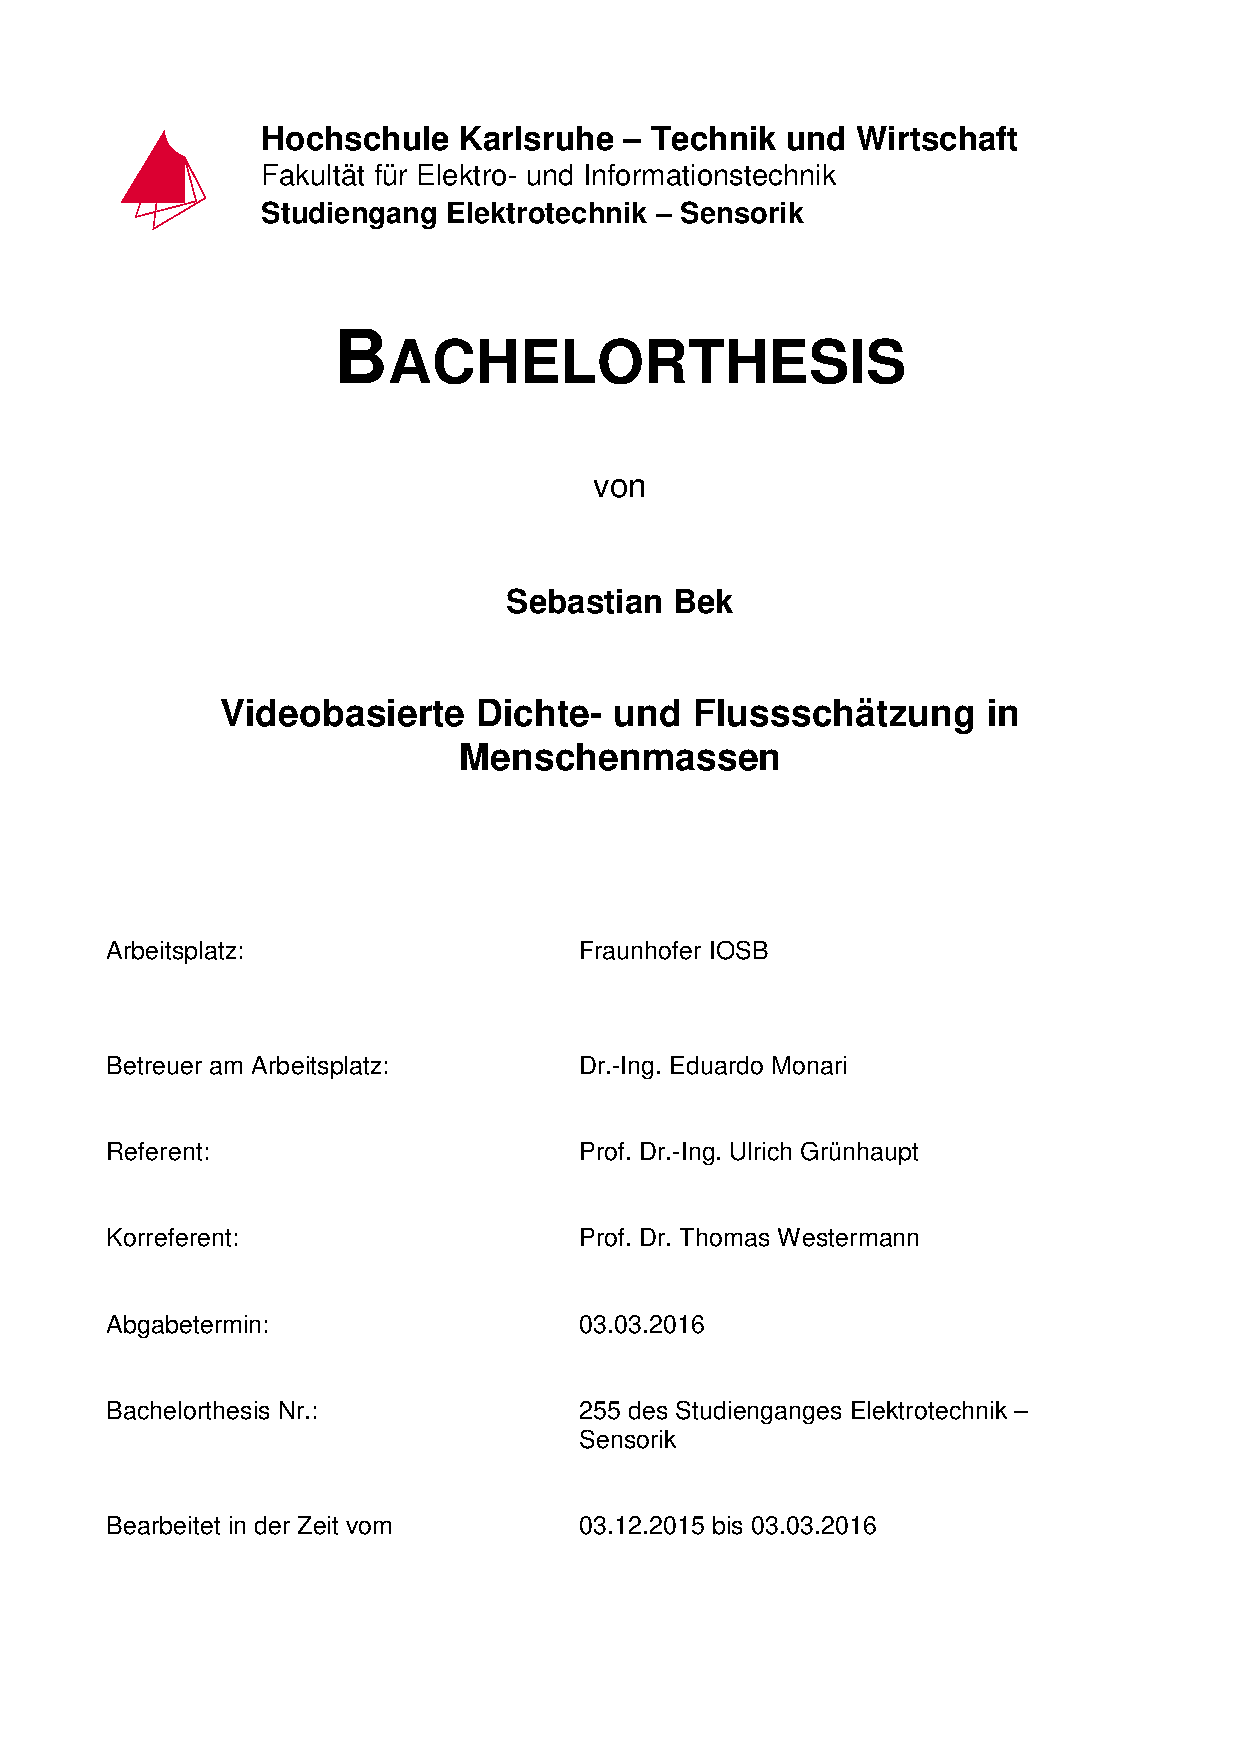
\includepdf[pages={1}]{./content/STB_Thesis_Deckblatt.pdf}

\prefrontmatter  %\pagenumbering{roman}%



%%% Verwendeter Literaturzitierstil
\bibliographystyle{abbrvdin}

%%%%%%%%%%%%%%%%%%%%%%%%%%%%%%%%%%%%%%%%%%%%%%%%%%%%%%%%
%%%%%% Nur für A4, nicht für A5
\addtolength{\marginparsep}{8pt}
\addtolength{\marginparwidth}{-20pt}

%%%%%%%%%%%%%%%%%%%%%%%%%%%%%%%%%%%%%%%%%%%%%%%%%%%%%%%%
%%%%%% Format des Deckblatts

% workaround, if removed title appears as background in externalized 
% % figures
  \tikzifexternalizing{}{
\ClearWallPaper


%%% Bei Diplomarbeiten etc.

\ifthenelse{\boolean{isdissertation}}{}{%
%%% Weitere Seite für die Erklärung der Selbstständigkeit
\begin{titlepage}
\thispagestyle{empty}

\ifthenelse{\boolean{iesenglishs}}{%
\chapter*{Statement of authorship}% %%PW
%% Andere Möglichkeiten
%% Own Work Declaration  %%sagt die Uni von Edinburgh
%% Affidavit  %% versicherung an eides statt
}{%
\chapter*{Erklärung der Selbstständigkeit}%
}
\thispagestyle{empty}
%% Text von hz Übernommen
\ifthenelse{\boolean{iesenglishs}}{%
I hereby declare that I have produced this work by myself except the utilities known to the supervisor, 
that I have labeled all used utilities completely and detailed and that I have labeled all material that has been taken with or without modification from the work of others.
}{%
Ich versichere hiermit, dass ich die vorliegende 
Bachelorthesis selbstständig erarbeitet und dabei 
keine anderen als die angegeben Quellen verwendet habe.}
%% Alternative
%Hiermit versichere ich, die vorliegende Arbeit selbstst�ndig verfasst und keine anderen als die angegebenen Quellen und Hilfsmittel benutzt sowie die Zitate deutlich kenntlich gemacht zu haben.
\vspace{4\baselineskip}\\
\ifthenelse{\boolean{iesenglishs}}{%
\Signplace, \Submissiondate \hfill \Authorname}{%
\Signplace, den \Submissiondate} \hfill \Authorname%
\vspace{4\baselineskip}\\
\clearpage
\mbox{}\thispagestyle{empty}
\end{titlepage}
}%
  }

\frontmatter %\pagenumbering{Roman}%
\newpage

\chapter*{Abstract}
\label{chap:Abstract}
%Sebastian
In den letzten Jahren erreichen uns immer häufiger Nachrichten über große Veranstaltungen, bei denen sich aufgrund zu hoher Besucherzahlen in Kombination mit unzureichender Planung Tumulte und Paniken, häufig mit Verletzten, ausbilden.
Solche Großveranstaltungen werden immer beliebter und sind fester Bestandteil der menschlichen Freizeitaktivitäten geworden, weswegen Einschränkungen Dieser unwahrscheinlich sind. Die Tendenz zeigt, das mit steigenden Besucherzahlen auch die Gefahr für Paniken und Unruhen steigt, weswegen videogestütztes Monitoring hier sinnvoll sein kann. Derzeit erfolgt das Monitoring von Veranstaltungen noch durch menschliche Betrachter, die oft unaufmerksam sind und meist nur subjektiv beurteilen können, wie hoch die Personenströme und -dichten wirklich sind. Zukünftig wird sich aber das automatisierte Monitoring durchsetzen, mit dem es möglich ist, ohne menschliches Eingreifen, Besucherzahlen und Personenströme quantitativ und relativ genau zu messen. Die automatische Erfassung und Analyse von Menschenströmen stellt jedoch zum heutigen Zeitpunkt noch eine technische Herausforderung dar.

In den ersten Jahren seines Lebens lernt der Mensch Formen, Strukturen und Kontouren richtig zu klassifizieren und aufgrund von Erfahrungswerten richtig einzuordnen. Mit diesen Erfahrungswerten, die sich über eine lange Entwicklung hin gebildet haben, kann der Mensch, mit einer sehr hohen Trefferquote, Personen als solche von anderen Strukturen in Bildern unterscheiden. Rechner und entsprechende Algorithmen sind hinsichtlich ihrer Erkennungsleistung noch lange nicht mit dem Menschen vergleichbar. Insbesondere bei niedriger Auflösung und starken Verdeckungsartefakten in der Szene, ist eine automatische Detektion von Personen mit den bekannten Verfahren bisher kaum möglich.

Im Gegenzug besitzt der Rechner, im Falle einer möglichen Detektion von Objekten, signifikante Vorteile bei der Analyse großer Datenmengen und bei der quantitativen Abschätzung von Messgrößen gegenüber der visuellen Auswertung. Um die Erkennungsleistung eines automatischen Systems, trotz der schwierigen Rahmenbedigungen bei der Beobachtung von Menschenmassen (niedrige Auflösung und Verdeckungen) auf ein einsetzbares Niveau zu steigern, werden im Rahmen dieser Arbeit Methoden basierend auf "`indirekten Merkmalen'', wie beispielsweise Bewegungsmerkmalen, untersucht, um auf Basis Dieser Informationen über die lokale Dichte und den lokalen Personenfluss innerhalb der Menschenmenge zu erschließen. Diese Dichte- und Flussinformationen sollen klassifiziert, quantifiziert und veranschaulicht werden, um etwaige Folgemaßnahmen bei kritischen Situationen zu erschließen. 
\newpage
Kurzfristige Folgemaßnahmen könnten \zb Evakuierung und Absperrung bestimmter Gebiete oder Eingriffe in Unruhen sein. Langfristige Folgemaßnahmen können \zb eine verbesserte Planung der Infrastruktur der Veranstaltung oder die Wahl eines größeren Veranstaltungsgeländes sein. Es soll ein Verfahren zur Erkennung und Messung der Bewegungs- und Gruppierungsmuster entwickelt und hinsichtlich seiner Performanz bewertet werden, um zu zeigen, dass es, auch unter Verwendung von niedrig aufgelösten Videodaten, für die Analyse von Dichte- und Flussinformationen in dicht gedrängten Personengruppen geeignet ist.



\setcounter{page}{1}
% Inhaltsverzeichnis in den PDF-Links eintragen
\newpage

\pdfbookmark[1]{Inhaltsverzeichnis}{toc}


%% PW: Protrusion fürs Inhaltsverzeichnis ausschalten (ist im Microtype Handbuch empfohlen)
\ifpdf
 \microtypesetup{protrusion=false}
\fi
\tableofcontents
\ifpdf
 \microtypesetup{protrusion=false}
\fi
\markboth{\empty}{\empty}

%% PW: Todo-Liste
% \listoftodos
%Symbol- und Abkürzungsverzeichnisse

\nomlabelwidth=15mm

%% Symbolverzeichnis
\markboth{Symbol- und Abkürzungsverzeichnisse}{Symbol- und Abkürzungsverzeichnisse}
\IfDefined{printnomenclature}{\printnomenclature}

\nomenclature{HG}{Hintergrund}
\nomenclature{VG}{Vordergrund}
\nomenclature{$\abs{\vec{a}}$}{Betrag eines Vektors}
\nomenclature{$\abs{\vec{b}}$}{Betrag eines Vektors der Bewegung über $q$ Frames}
\nomenclature{$v(x,y)$}{Merkmalsgeschwindigkeit}
\nomenclature{$v_{SI}(x,y)$}{Merkmalsgeschwindigkeit in SI-Einheiten}
\nomenclature{$d(x,y)$}{Abstand zwischen 2 Pixeln in $\frac{m}{px}$}
\nomenclature{$D$}{fraktale Dimension}
\nomenclature{$FR$}{Framerate - Bildfrequenz in $[\text{fps}] = [\frac{\text{frame}}{s}]$}
\nomenclature{c}{Center Pixel/Hotspot, auf den sich eine Nachbarschaft/Umgebung oder ein Patch/Bildausschnitt bezieht}
\nomenclature{ROI}{region of interest - Vordergrundregion(\zb Positionen oder Polygonzüge)}
\nomenclature{HSV}{hue, saturation, value - Farbmodell, für intuitivere Definition von Farben}
\nomenclature{$w(u,v)$}{Fenster-/Wichtungsfunktion}
\nomenclature{$W(u,v)$}{Wertebereich für die Laufvariablen $u$ und $v$ innerhalb eines Bildausschnitts konstanter Größe in $[\text{px}]$}
\nomenclature{$W(w,h)$}{Wertebereich für die Bildkoordinaten $x$ und $y$ innerhalb eines Bildausschnitts festgelegter Größe in $[\text{px}]$}
\nomenclature{$w$}{Breite(width) eines Bildausschnitts}
\nomenclature{$h$}{Höhe(height) eines Bildausschnitts}
\nomenclature{$I(x,y)$}{Intensitäts-/Bildmatrix}
\nomenclature{$I_x$}{diskrete Ableitung der Intensitätsmatrix in x-Richtung in $[\frac{1}{\text{px}}]$}
\nomenclature{$I_y$}{diskrete Ableitung der Intensitätsmatrix in y-Richtung in $[\frac{1}{\text{px}}]$}
\nomenclature{$M$}{Kovarianzmatrix der Verteilung von Gradientenbeiträgen $I_x$,$I_y$}
\nomenclature{$\lambda_{1/2}$}{Eigenwerte der Matrix A}
\nomenclature{$DX$}{DX-Wert eines Verschiebungsvektors in $[\text{px}]$}
\nomenclature{$DY$}{DY-Wert einer Verschiebungsvektors in $[\text{px}]$}
\nomenclature{$c_K$}{Konstante}
\nomenclature{$j$}{Index für den aktuellen Frame}
\nomenclature{$m$}{Mittelungsdistanz - Anzahl der rückwärtigen Messwerte $m$, die in die Mittelung einbezogen werden in $[\text{frame}]$}
\nomenclature{$x,y$}{Bildkoordinaten - Breite, Höhe}
\nomenclature{$P(x,y)$}{Zeilen-/Spaltenposition im Eingangsbild}
\nomenclature{$P_j(x)$}{x-Position im Eingangsbild im aktuellen Frame j}
\nomenclature{$\text{var}()$}{Varianz}
\nomenclature{$\text{covar}()$}{Kovarianz}
\nomenclature{$u,v$}{Laufvariablen für die Verschiebung in Zeilen- und Spaltenrichtung}
\nomenclature{$A$}{projezierte Fläche eines Bildausschnitts in $[m^2]$}
\nomenclature{$S$}{Menge an Trajektorienspitzen(aktuelle Position) im Patch}
\nomenclature{$K$}{Menge an Trajektorienknoten(vorherige Position) im Patch}
\nomenclature{$Z$}{Menge an berechneten Vektorlängen $\abs{\vec{b}}_j(x,y)$ im Patch}
\nomenclature{$N$}{Personenzahl in $[\text{personen}]$}
\nomenclature{$\bar{N}_j$}{mittlere Personenzahl im aktuellen Frame j in $[\text{personen}]$}
\nomenclature{$N_{max}$}{trainierte maximale Personenzahl in $[\text{personen}]$}
\nomenclature{$N_{abs}$}{absolute maximale Personenzahl in $[\text{personen}]$}
\nomenclature{$N_{rel}$}{relative mittlere Personenzahl in $[\%]$}
\nomenclature{$D_{scal}$}{skalierte Personendichte in $[\frac{\text{personen}}{m^2}]$}
\nomenclature{$N_{scal}$}{skalierte Personenzahl in $[\text{personen}]$}
\nomenclature{$F_{acc}$}{Fluss-Akkumulator in $[\frac{\text{personen}}{\text{frame}}]$}
\nomenclature{$F$}{Personenfluss in $[\frac{\text{personen}}{\text{frame}}]$}
\nomenclature{$\bar{F}_j$}{mittlerer Personenfluss in $[\frac{\text{personen}}{\text{frame}}]$}
\nomenclature{$F_{rel}$}{relativer mittlerer Personenfluss $[\%]$}
\nomenclature{$F_{max}$}{trainierter maximaler mittlerer Personenfluss $[\%]$}
\nomenclature{$F_{scal}$}{skalierter Personenfluss in $[\frac{\text{personen}}{\text{frame}}]$}
\nomenclature{$B_j$}{mittlere Merkmalsgeschwindigkeit innerhalb eines Bildausschnitts in $[\frac{px}{q\cdot \text{frame}}]$}
\nomenclature{$B_S$}{niedrigster Schwellwert für die mittlere Merkmalsgeschwindigkeit in $[\frac{px}{q\cdot \text{frame}}]$}
\nomenclature{$\bar{B}_j$}{zeitlich gemittelte mittlere Merkmalsgeschwindigkeit innerhalb eines Bildausschnitts}
\nomenclature{$\bar{B}_{rel}$}{relative mittlere Merkmalsgeschwindigkeit innerhalb eines Bildausschnitts in $[\%]$}
\nomenclature{$\text{dFactor}$}{Dichtefaktor in $[\%]$}
\nomenclature{$X_{rel}$}{relative Messgröße allgemein in $[\%]$}
\nomenclature{$\text{hue}$}{hue: zahlenmäßiger Farbton im HSV-Farbmodell in  $[\ ]$}

\nomenclature{$r$}{Suchradius in $[\text{px}]$}
\nomenclature{$p$}{Schrittweite in $[\text{frame}]$}
\nomenclature{$q$}{Schrittweite in $[\text{frame}]$}

\nomenclature{$d_1$}{Abstand der unteren Bildzeile zum Kameraobjektiv in $[m]$}
\nomenclature{$d_2$}{Abstand der oberen Bildzeile zum Kameraobjektiv in $[m]$}



% später dann evtl. \markboth{\empty}{\empty} nötig (http://www.golatex.de/falsche-kopfzeile-im-abkuerzungsverzeichnis-t2074.html)


% Hauptteil
\mainmatter
\hypersetup{pageanchor=true}

%%%%%%%%%%%%%%%%%%
%%%%%%%%%%%%%%%% HIER KOMMEN DIE EINZELNEN QUELLDATEIEN DES AUTORS REIN!!
%includes sind nicht hierarchisch, input schon
%\input{./content/0-Anleitung}
% Einleitung
% o	Stand der Forschung
% o	(Grundlagen)
% Vorbereitung
% o	Implementierung
% ·         Konzept
% §  Trainingsdaten / Annotation / Klassifikation
% ·         Merkmalsextraktion
% §  Beschreibung der umgesetzten Features und Variationen
% ·         Klassifikation
% ·         Sonstiges…
% o	Bewertung / Ergebnisse
% ·         Trainingsdaten / Evaluationsdaten
% ·         Bewertung der Merkmale
% ·         Bewertung der "Invarianz des Verfahrens"
% ·         Bewertung Nutzen des "Aufblähens der Trainingsdaten"
% ·         Bewertung Kombination der Merkmale
% ·         Rechenzeit


\chapter{Einleitung}
\label{chap:ein}

%Sebastian
Diese Arbeit befasst sich mit der algorithmischen Detektion und Messung von Bewegungs- und Gruppierungsmustern von Personen, wobei Trajektorien (Pfade) als Grundlage für die darauf aufsetzende Dichte- und Flussschätzung verwendet werden. Besonders intensiv werden dabei die Personenzählung (in Personen/Bildausschnitt), die Berechnung einer mittleren Strömung (in Personen/Frame) und die Ableitung eines Dichtefaktors (in \% einer Maximaldichte) in einem bestimmten Bildausschnitt behandelt. Das Verfahren soll in Kombination mit Anderen in Form einer integrierten Software zur komfortablen Analyse von Gruppierungs- und Bewegungsmustern und zur Einrichtung von Schnellwarnsystemen eingesetzt werden.

Der nachfolgende Abschnitt (\ref{sec:motiv}) befasst sich mit der Motivation für die automatisierte Videoauswertung. Er basiert auf der Dissertation "`Automatische Erfassung präziser Trajektorien in Personenströmen hoher Dichte'' von Maik Boltes \cite{boltes} und dem Artikel "`A Method for Counting Moving People in Video Surveillance Videos'' von Donatello Conte et al. \cite{conte}. Anschließend werden die Ziele dieser Arbeit (s. Abschnitt \ref{sec:ziele}) und im folgenden Abschnitt \ref{sec:std} der aktuelle Stand der Technik behandelt.

%%%%%%%%%%%%%%%%%%%%%%%%%%%%%%%%%%%%%%
\section{Motivation}
\label{sec:motiv}

Personenströme und -anordnungen im Alltag sind für uns gewöhnliche Abläufe, die aber dennoch interressante Erkenntnisse über die Selbstorganisation und die Gewohnheiten der Menschen liefern können. Zudem wäre es mit Sicherheit von Vorteil ein tiefgreifendes Verständnis der bisher nur grob erforschten Dynamik von Personenströmen zu gewinnen, um Beobachtungen zu machen, die in sicherheitskritischen und ökonomischen Anwendungsgebieten hilfreich sein können. 
\newpage
Die Erfassung dicht gedrängter Personengruppen mit Kameras und Bildauswertungssoftware erweist sich dabei als besonders zielführend, da analysierte Szenen vom Computer direkt ausgewertet und die angezeigten Informationen aufbereitet werden können. An das Personal werden dabei geringere Anforderungen an Aufmerksamkeit und Organisation gestellt. Es können außerdem Messdaten aufgenommen und quantitative Aussagen über das Verhalten von Personengruppen gemacht werden.

Gestützte Monitoringssysteme sind vor allem an Orten, die von vielen Menschen gleichzeitig besucht werden (\zb Großveranstaltungen oder Fußgängerzonen) sinnvoll. Denn mit höheren Besucherzahlen nimmt möglicherweise auch das Risiko für Schadensereignisse oder Kriminalität zu, weil die Zahl an Personen, die bereit sind Verbrechen zu begehen und Tumulte zu verursachen, mit der Besucherzahl steigt. Solche Großveranstaltungen bergen zudem die Gefahr für Massenpaniken, weswegen als Grundsatz für eine Veranstaltungsplanung Flucht- und Rettungswege ausnahmslos freigehalten werden sollten. Langfristig kann mit flächigem videogestütztem Monitoring die Planung verbessert werden, indem \zb kritische Gebiete entlastet werden (breitere Tore/Türen, Fluchtwege) oder die Zeitplanung für die öffentlichen Verkehrsmittel überdacht wird. Für kurzfristige Reaktionen kann mit der integrierten Software ein Schnellwarnsystem, in Form eines Kameranetzwerkes, am Veranstaltungsort installiert werden, das schnell ortsbezogene Notrufe tätigen und exakte Positionen von besonders kritischen Gebieten des Veranstaltungsgeländes übermitteln kann. Kritische Gebiete sind zum Beispiel Staugebiete, also Orte, an denen die Personenzahl hoch ist und eine geringe Dynamik herrscht. Ein solches Schnellwarnsystem sollte kritische Situationen schnell erkennen und melden können, weswegen als Vorraussetzung die Extraktion der Laufwege auch bei hohen Personendichten (, die kritischen Situationen entsprechen,) verlässlich anwendbar sein muss.
Außerdem ist es möglich, durch eine Kalibrierung der Kameras, georegistrierte Messwerte zu erhalten, die beispielsweise auf einer Karte oder Aufnahme des Veranstaltungsgeländes dargestellt werden können. Dies ermöglicht eine einfache visuelle Auswertung der Daten, die geringe Anforderungen an die Aufmerksamkeit der Nutzer stellt. Die Daten können entweder in Echtzeit oder im Nachhinein zur verbesserten Planung analysiert werden. Zusätzlich kann das aufgenommene Beweismaterial zu Rate gezogen werden, wenn Unklarheiten über die Ursache für den sicherheitskritischen Fall bestehen. Dies sollte aber ohne Identifizierung von Einzelnen erfolgen.

%Neue Seite?
%%%%%%%%%%%%%%%%%%%%%%%%%%%%%%%%%%%%%%
\section{Aufgabenstellung und Ziele}
\label{sec:ziele}
In dieser Arbeit wird die Untersuchung und Entwicklung eines Videoanalyseverfahrens zur automatischen Extraktion von Trajektorien (Pfaden) bewegter Personen behandelt. Das Verfahren soll im Rahmen eines Videoanalysesystems, das für die Realisierung eines Schnellwarnsystems und für die komfortable Analyse von Bewegungs- und Gruppierungsmustern (s. Abschnitt \ref{sec:motiv}) zur Langzeitplanung von Veranstaltungen geeignet ist, entwickelt und dokumentiert werden. 
\newpage

Es sollen Laufwege bewegter Personen, deren Ecken zuvor algorithmisch detektiert wurden, als Bildkoordinaten in Listen eingetragen und verwaltet werden. Solche Laufwege werden als Trajektorien bezeichnet. Dabei sollen nur bewegte Eckpunkte verwendet werden, weswegen gänzlich stillstehende Personen (zunächst) nicht erfasst werden. Weiterhin können aus den gespeicherten Positionen der Trajektorien, innerhalb von bestimmten Bildausschnitten, Messgrößen wie Personenfluss, Personenzahl und Dichtefaktoren abgeleitet werden. Das Verfahren sollte zuverlässig sein und keine auffälligen, kritischen Situationen übersehen. Es soll erprobt und mithilfe von Grundwahrheiten bewertet werden, um eine Aussage über die Wahrheitstreue der Messgrößen treffen zu können.


%\\ \\
%Nachfolgend werden Vor- und Nachteile der Nutzung von Bildauswertungssoftware gegenüber manueller Videoüberwachung erfasst:

%\begin{center}
%\fbox{
%\begin{minipage}[t]{0.47\textwidth}
%\begin{center}
%\bigskip
%\textbf{Vorteile}:
%\bigskip
%\hline
%\end{center}
%\begin{itemize}
%\item[+] System benötigt geringeren Personaleinsatz
%\item[+] komfortable Videoüberwachung
%\item[+] quantitative Aussagen(ohne subjektiven Einfluss) möglich
%\item[+] System hat keinen Konzentrationsverlust
%\item[+] System übersieht in der Regel keine Gefahren
%\end{itemize}
%\bigskip
%\bigskip
%\bigskip
%\end{minipage}
%\hskip 5pt
%\vline
%\hskip 7pt
%\begin{minipage}[t]{0.47%\textwidth}
%\begin{center}
%\bigskip
%\textbf{Nachteile}:
%\bigskip
%\hline
%\end{center}
%\begin{itemize}
%\item[-] unflexible Reaktion des Systems auf Szenenwechsel
%\item[-] System löst Falschalarme aus
%\item[-] System besitzt keine menschlichen Erfahrungswerte
%\item[-] Leistung des Systems ist hardwareabhängig
%\item[-] aufwendige Kalibrierung des Systems
%\end{itemize}
%\bigskip
%\end{minipage}
%\bigskip
%\bigskip %\%\
%}
%\end{center}


%%%%%%%%%%%%%%%%%%%%%%%%%%%%%%%%%%%%%%
\section{Stand der Technik}
%Bei Anne geht es mehr um Segmentierung - hier mehr um Erstellung von Trajektorien(Tracking) der Personen
\label{sec:std}

Die Idee, automatische Videoanalyseverfahren zur Erkennung von Mustern und Objekten einzusetzen, ist keine neue Vorstellung. Wegen der zunächst nur wenig fortgeschrittenen Technik, setzte sich diese Idee jedoch erst in den 1980er Jahren durch. Heute gibt es vielseitige Ansätze, um diese Aufgaben zuverlässig durchzuführen. Dennoch haben diese Verfahren ihre Grenzen und es existiert ein weitreichendes Verbesserungspotenzial.

Wie in Abschnitt \ref{sec:ziele} beschrieben, wird in dieser Arbeit die algorithmische Detektion und Messung von Dichte- und Flussinformationen in Personengruppen behandelt. Um solche Gruppierungs- und Bewegungsmuster erfassen und messen zu können, müssen die Personen zunächst quantitativ erfasst werden. Zur Zählung von Personen/Objekten existieren, nach aktuellem Stand, zwei grundlegende Ansätze. Zunächst muss, in beiden Fällen, eine Extraktion einer ROI (region of interest - \zb Punkte, Flächen) zur groben Ausfilterung von uninteressanten Bereichen, an denen sich gerade keine Personen befinden können, vorgenommen werden. Dabei werden uninteressante, statische Bereiche im Bild ausgefiltert, während die interessanten Bereiche hinsichtlich Personendetektion, Dichte- und Flussschätzung weiterverarbeitet werden. Nachfolgend werden die beiden Ansätze beschrieben und mit Beispielen ausgeführt.

%\subsection{Extraktion einer ROI}
% Zur Extraktion einer ROI gibt es derzeit einige Möglichkeiten, wobei die Wichtigsten nachfolgend aufgezählt werden:

%\subsubsection{Segmentierungsverfahren:}

%\begin{itemize}

%\item Pixelorientierte Verfahren: Diverse Schwellwertverfahren eignen sich zur Segmentierung, wenn die Dichte der Grauwerte im Histogramm ausreichend bimodal ist(s. Otsu-Schwellwertverfahren %\cite{segcourse}).

%\item Kantenorientierte Verfahren: Diverse Kantenfilter, wie Scharr- und Sobel-Operator eignen sich zur Segmentierung, wenn anschließend ein "`Flood-Fill-Algorithmus'' eingesetzt wird, um den Hintergrund zu fluten. %\cite{segcourse2}

%\item Modellbasierte Verfahren: Diverse geometrische Modelle wie Kreise oder Geraden eignen sich zur Segmentierung, wenn beispielsweise die Form der Kanten mit ihnen verglichen wird. %\cite{segcourse2}

%\item Regionenorientierte Verfahren: Diese Verfahren wählen Pixelpositionen als Ausgangspunkte und lassen Vordergrundregionen nach verschiedenen Kriterien wie Ähnlichkeit ausgehend von dieser Position wachsen oder sich vereinen. %\cite{segcourse2}

%\item Texturorientierte Verfahren: Texturen in Vordergrund-Regionen werden erkannt und anhand ihrer Beschaffenheit interpretiert. Unruhige Strukturen deuten %\zb auf Personengruppen und Glatte auf eine leere Oberfläche hin(s. "`Haar-Wavelets'' oder "`gray-level-co-occurence-matrix'' %\cite{segcourse2}).

%\item Selektion des Hintergrunds: Der Hintergrund wird erfasst und subtrahiert(Subtraktion des Hintergrunds). Der Hintergrund wird abgezogen und erhält somit idealerweise die Farbe Schwarz, während der Vordergrund erhalten bleibt. Wie in %\cite{zhao} beschrieben, kann Hintergrund zum Beispiel detektiert werden, indem statische Regionen im Bild markiert werden. 

%\item Detektion mit Sensor-Array/3D-Kameras: Eine Szene wird mit einer 3D-Kamera gefilmt, um die räumliche Struktur zu dokumentieren und 3D-Objekte zu segmentieren, die als 3D-Modelle gespeichert werden.

%\end{itemize}

%\subsubsection{Merkmalsdetektionsverfahren}

%\begin{itemize}
    %\item Extraktion von Vordergrund-Merkmalen("`Features'' - \zb Punkten), die beispielsweise durch extrahierte Eckpunkte(s. "`Harris Corner Detector'') gegeben sind und in Kombination mit einer Bewegungsschätzung (optischer Fluss) als lokale Bewegungsmerkmale verwendet werden können.
%\end{itemize}

\subsection{direkter Ansatz}
\begin{enumerate}
\item Segmentierung von VG-Bereichen: nach Möglichkeit mit beinhalteten Personen
\item Detektion und individuelle Separation der Personen
\item Zählung der separierten Vordergrund-Regionen
\end{enumerate}

Im Fall des direkten Ansatzes, werden in Kombination zur Extraktion einer ROI in VG-Regionen Muster und Merkmale gesucht, die Menschen zugeordnet werden sollen, um diese einzeln zu separieren. 
\newpage
Nachfolgend werden einige Beispiele für den direkten Ansatz aufgeführt:
\vskip 10pt
\emph{Objektklassifizierung:}
\begin{itemize}

\item Vergleich der Form: Kanten von Vordergrund-Regionen werden mit Modellen (Rechtecke, Ellipsen o.ä.), die entweder ganze Menschen oder Körperteile modellieren, verglichen (s.\cite{rittscher}).

\item Vergleich der Kantenstatistik: Anzahl, Ausrichtung und Form der Kanten können Menschen beschreiben, wobei Statistiken/Histogramme über die Häufigkeit von Kantenrichtungen erstellt und gespeichert werden, falls sich ein/kein Mensch im Bildausschnitt befindet (s. HOG = histogram of oriented gradients). Anschließend kann, über einen Vergleich der Kantenstatistik des analysierten Bildausschnitts mit der gespeicherten Kantenstatistik, entschieden werden, ob ein Mensch in einem Bildausschnitt befindlich ist. Dies wird von einem lernenden Algorithmus (SVM: support vector machine) durchgeführt. Zusätzlich kann hier, wie in \cite{loy2013crowd} beschrieben, bestimmt werden, ob sich gerade mehr (komplexere Kanten) oder weniger Menschen (einfache Kanten) in einem größeren Bildausschnitt aufhalten.

\item Vergleich von aufgenommenen 3D-Modellen mit Standardmodellen: Nach \cite{zhao} können Menschen erkannt werden, indem ein 3D-Modell, das mit einer 3D-Kamera oder einem Sensor-Array erstellt wurde, mit Standardmodellen für Menschen verglichen wird.

\item Gruppieren von extrahierten Merkmalen ("`Features'' - \zb Punkten) nach ihren Bewegungscharakteristika: Punkte, die sich nahezu gleich schnell in eine Richtung bewegen, gehören mit hoher Wahrscheinlichkeit nur zu einer Person (s. \cite{brostow}).

\end{itemize}
\vskip 5pt
Anschließend wird, über ein Labeling-Verfahren (\zb ein sog. "`Point Clustering''), eine Vergabe von Identifikationsnummern durchgeführt, wobei die einzeln (als Vordergrund-Regionen) separierten Personen mit IDs versehen und gezählt werden können.

Beim nachfolgenden indirekten Ansatz wird eine solche Objektklassifizierung nicht durchgeführt, sondern direkt mit der extrahierten ROI gearbeitet.

\subsection{indirekter Ansatz}

\begin{enumerate}
\item Detektion und Extraktion von lokalen Merkmalen (segmentierungslos - \zb Punkte/Pixelpositionen), die beispielsweise durch extrahierte Eckpunkte (s. "`Harris Corner Detector'' \cite{albiol}) gegeben sind und in Kombination mit einer Bewegungsschätzung (optischer Fluss) als lokale Bewegungsmerkmale verwendet werden können.
\item Ableitung der Personenzahl aus der Zahl der lokalen, extrahierten Merkmale, unabhängig von einer separaten Detektion von Personen
\end{enumerate}

Dieser Ansatz gilt als robuster, weil die vereinzelte Separation der Personen, besonders in überfüllten Gebieten, ein zu großes Problem darstellt und bisher nicht zuverlässig gelöst wurde.
\vskip 5pt
Nachfolgend werden einige Beispiele für den indirekten Ansatz aufgelistet:

\begin{itemize}

\item Zählen der Menge an nicht-statischen Pixeln (s. \cite{cho})

\item Zählen der Menge an nicht-statischen Eckpunkten, extrahiert von einem Corner Detector (\zb Harris Corner Detector, wie in \cite{albiol} beschrieben)

\item Erfassen der Größen und Häufigkeiten von VG-Bereichen (vgl. \cite{kong})

\item Erfassen der fraktalen Dimension von VG-Bereichen (vgl. \cite{marana}):\\
\begin{center}
$D = \frac{\text{log(Zahl der selbstähnlichen Bestandteile)}}{\text{log(Abbildungsmaßstab)}}$
\end{center}
\end{itemize}

\vskip 5pt
In dieser Arbeit wird eine Ausführung des indirekten Ansatzes behandelt. Dabei kommt der Harris Corner Detector, wie in \cite{albiol} beschrieben, zum Einsatz, um Eckpunkte/Merkmale zu extrahieren und vom Hintergrund zu trennen. Ein Corner Tracker erfasst die relative Bewegung (den optischen Fluss) dieser Merkmale entlang der Bildzeilen und -spalten. Die Anzahl an bewegten Personen wird in ein Verhältnis mit der Anzahl an sich bewegenden, extrahierten Eckpunkten gesetzt und daraus werden weitere Größen wie Personenfluss und ein Dichtefaktor abgeleitet.

Wichtige Verfahren, in Bezug auf diese Arbeit, sind somit zunächst der Harris Corner Detector, gekoppelt an einen Corner Tracker, der die Bewegung (den optischen Fluss) erfasst, sowie das Verfahren zur Erfassung von Trajektorien (Pfaden) der extrahierten Eckpunkte. Diese Grundlagen werden im Kapitel \ref{chap:grund} näher erläutert. Diese Arbeit soll zeigen, dass das entwickelte Verfahren, auch mit den niedrig aufgelösten Daten \zb von CCTV-Überwachungskameras, in Personengruppen hoher Dichte zuverlässig angewandt werden kann.




\chapter{Grundlagen}
\label{chap:grund}

Dieses Kapitel befasst sich mit den Basismethoden, welche in den untersuchten Verfahren eingesetzt werden. Zunächst wird in Abschnitt \ref{sec:harris} das zugrundeliegende Verfahren zur Extraktion lokaler Bildmerkmale beschrieben, das auf dem Harris Corner Detector \cite{collinscourse} basiert. Anschließend wird im Abschnitt \ref{sec:corner} der verwendete Corner Tracker behandelt, welcher zu den lokalen Bildmerkmalen Bewegungsinformationen (vgl. Abschnitt \ref{sec:planes}) hinzufügt (motion vectors - Bewegungsvektoren). Im letzten Abschnitt \ref{sec:trajektorien} wird das verwendete Verfahren zur Erfassung von Trajektorien (Pfaden) der lokalen Bildmerkmale, und dadurch indirekt der Personen (-gruppen), näher beschrieben.

\section{Harris Corner Detector}
\label{sec:harris}
Der "`Harris Corner Detector'' \cite{collinscourse} ist ein Algorithmus, der verschiedene Bildausschnitte (Patches) einer Bildmatrix $I$ nach Ecken (engl.: Corners) durchsucht und diese in Form der Position des Center Pixels extrahiert, falls sich eine Ecke im Bildausschnitt befindet. Eine grafische Beschreibung der Idee des Harris Corner Detector wird auf der folgenden Seite dargestellt. Dabei werden unterschiedliche Patches (s. Abbildung \ref{gradient} - blau) mit unterschiedlichen Situationen betrachtet:

\begin{figure}[H]
\centering
  \begin{minipage}{0.3\textwidth}
    
\includegraphics[width=\textwidth]{images/dummy.png}
    \label{a)}
  \end{minipage}
  \begin{minipage}{0.3\textwidth}
    
\includegraphics[width=\textwidth]{images/dummy.png}
    \label{b)}
  \end{minipage}
  \begin{minipage}{0.3\textwidth}
    
\includegraphics[width=\textwidth]{images/dummy.png}
    \label{c)}
  \end{minipage}
\caption{Betrachtung der Gradientenbeiträge verschiedener Patches}
\label{gradient}
\end{figure}

%BILD Patch im flachen und auf einer Ecke
Diese anschauliche Beschreibung der Idee des Harris Corner Detectors zeigt, dass in der Umgebung einer Ecke immer viele hohe Intensitätsunterschiede (Gradientenbeiträge) in verschiedene Richtungen vorliegen. In Abbildung \ref{harris} werden Verteilungen der Gradientenbeiträge in x- und y-Richtung für die verschiedenen Fälle in einem Bildausschnitt betrachtet:
\bigskip
\bigskip
\begin{figure}
  \centering
  \fbox{
    
\includegraphics[width=0.8\textwidth]
    {images/dummy.png}
  }
  \caption{Verteilungen von Gradientenbeiträgen $I_x,I_y$ \cite{collinscourse}}
  \label{harris}
\end{figure}
\newpage
Dabei wird klar, dass je nach Situation eine andere Verteilung der Daten vorliegt und zwischen allen drei Fällen klar unterschieden werden kann. Dafür muss aber unterschieden werden können, ob die Varianz der Verteilung mit Bezug zum Ursprung generell klein (im Fall einer Fläche), groß in eine Richtung (im Fall einer Kante) oder groß in mindestens 2 Richtungen (im Fall einer Ecke) ist. Dazu wird eine Kovarianzmatrix (auch bekannt als Strukturtensor) $M$ für die Verteilung der Gradientenbeiträge $I_x$,$I_y$ hergeleitet (Herleitung siehe \cite{cscourse}), die die Varianz der Daten mit Bezug zum Ursprungswert ($I_x=0$, $I_y=0$) im aktuellen Bildausschnitt mit Center Pixel $x,y$ beschreibt:

\begin{align}
M = \sum_{u,v}{w(u,v)
\begin{bmatrix}
I_x^2 & I_xI_y\\
I_xI_y & I_y^2\\
\end{bmatrix}
}
&=
\begin{bmatrix}
a = \sum_{u,v}{w(u,v)I_x^2} & b = \sum_{u,v}{w(u,v)I_xI_y}\\
b = \sum_{u,v}{w(u,v)I_xI_y} & c = \sum_{u,v}{w(u,v)I_y^2}\\
\end{bmatrix}
\notag \\ \bigskip \bigskip \bigskip
\begin{bmatrix}
a & b\\
b & c\\
\end{bmatrix}
&=
\begin{bmatrix}
\text{var}(I_x) & \text{covar}(I_x,I_y)\\
\text{covar}(I_x,I_y) & \text{var}(I_y)\\
\end{bmatrix}
\end{align}
\vskip 5pt
\begin{flushleft}
mit  $u,v \in W(u,v)$, $I_x=I_x(x+u,y+v)$ und $I_y=I_y(x+u,y+v)$
\end{flushleft}
\vskip 5pt
$I_x$ und $I_y$ werden wegen der kompakteren Schreibweise abgekürzt.
$w(u,v)$ ist hier eine Gewichtungsfunktion wie die Rechteck- oder Gauss-Funktion. $W(u,v)$ beschreibt den zulässigen Wertebereich, innerhalb dem $u$ und $v$ liegen müssen, um den definierten Bildausschnitt nicht zu überschreiten. Für die Eigenwerte der Matrix $M$ gilt:
\begin{equation}
\lambda_{1/2} = \frac{a+c \pm \sqrt{(a-c)^2 + 4b^2}}{2}
\end{equation}
Im Fall einer Kovarianzmatrix geben die Eigenvektoren Dieser die 2 orthogonalen Hauptrichtungskomponenten der Varianz der Daten an. Die Eigenwerte $\lambda_1$ und $\lambda_2$ beschreiben die Länge der größten Eigenvektoren und damit die Varianz der Verteilung von $I_x$, $I_y$ in Richtung der Eigenvektoren. Damit ergeben sich im Falle einer:
\begin{itemize}
\item flachen Region (s. Abbildung \ref{harris} - flat): 2 kleine Eigenwerte der Matrix B (keine Varianz) $\Rightarrow \lambda_1\sim \lambda_2\approx 0$ 
\item Kantenregion (s. Abbildung \ref{harris} - edge): 1 großer, 1 kleiner Eigenwert der Matrix B (große Varianz in eine Richtung) $\Rightarrow \lambda_1 >> \lambda_2$ \hskip 5pt $v$ \hskip 5pt $\lambda_2 >> \lambda_1$
\item Eckregion (s. Abbildung \ref{harris} - corner): 2 große Eigenwerte der Matrix B (große Varianz in mindestens 2 Richtungen) $\Rightarrow \lambda_1\sim \lambda_2$ 
\end{itemize}

\newpage

Um in allen Fällen verschiedene Ergebnisse zu erhalten, wird eine sogenannte Corner Response an jedem Pixel definiert, die große, positive Werte für Ecken, große Negative für Kanten und kleine Werte für flache Regionen annimmt:
\begin{equation}
R = \lambda_1\lambda_2 - k(\lambda_1 + \lambda_2)^2
\end{equation}
$k$ ist ein empirisch festgelegter Parameter, dessen Wertebereich zwischen 0,04 und 0,06 liegt.
Um den Rechenaufwand, der durch die Berechnung der Eigenwerte entsteht (Quadratwurzeln sind rechenintensiv) zu verringern, wird die Corner Response oft so definiert:
\begin{equation}
R = \det{B} - k(\text{spur\ } B)^2
\end{equation}
mit: $\det{B} = \lambda_1\lambda_2$ und $\text{spur\ } B = \lambda_1+\lambda_2$\\

\section{Corner Tracker}
\label{sec:corner}
Als Grundlage der Arbeit liegt eine Bibliothek "`OCV\_CornerTracker'' vor, in der im Rahmen eines sogenannten Corner Trackers der Harris Corner Detector bereits implementiert ist. Das Blockschaltbild dieser Bibliothek wird in Abbildung \ref{ocv} dargestellt.
\bigskip
\begin{figure}[h]
  \centering
  \fbox{
    
\includegraphics[width=0.7\textwidth]
    {images/dummy.png}
  }
  \caption{Blockschaltbild: OCV\_CornerTracker}
  \label{ocv}
\end{figure}
\begin{flushleft}
\underline{Funktion:}
\end{flushleft}
Das hier eingesetzte Verfahren zum Tracking von Harris Corner Features (Merkmalen) berechnet zunächst für jeden Pixel im vorherigen (n-1.) Eingangsbild den sogenannten optischen Fluss \cite{Baker07adatabase}. Dabei wird ein Intensitätsprofil aus der Umgebung eines Pixels erstellt. Dieses Profil wird in der Umgebung des Pixels im aktuellen (n.) Eingangsbild gesucht. Die relative Verschiebung des Mittelpunkts im Profil im Vektorraum, zwischen beiden Eingangsbildern, gibt den optischen Fluss des Pixels in Zeilen- und Spaltenrichtung an. 
\newpage
In Abbildung \ref{gaussians} werden beispielhaft solche Verschiebungsvektoren in einem Videobild in blau eingezeichnet. Anschließend wird zu den jeweiligen Pixelpositionen, die im vorherigen (n-1.) Eingangsbild als Harris Corners klassifiziert wurden, der zugehörige optische Fluss als Bewegungsschätzung hinzugefügt. An Positionen, an denen die Merkmale keine Bewegungen aufweisen oder keine Merkmale extrahiert wurden, werden die Verschiebungsvektoren gleich 0 gesetzt. Zusammenfassend enthalten die generierten Verschiebungsvektoren ausschließlich pixelbezogene Bewegungen der extrahierten Merkmale des Harris Corner Detectors vom letzten (n-1.) zum aktuellen (n.) Frame.
\vskip 5pt
\begin{figure}[h]
  \centering
  \fbox{
    
\includegraphics[width=0.75\textwidth]
    {images/dummy.png}
  }
  \caption{optischer Fluss von detektierten Ecken an Marathonläufern \cite{AliS07}}
  \label{gaussians}
\end{figure}

\section{Verschiebungsvektoren}
\label{sec:planes}

Die Verschiebungsvektoren, die vom Corner Tracker (s. Abschnitt \ref{sec:corner}) ausgegeben werden, beinhalten die relativen Bewegungen der extrahierten Merkmale in Zeilen- und Spaltenrichtung am Ort des Ursprungs. Aus den beiden Vektorkomponenten können für jede detektierte Position im Bild Vektorbeträge berechnet werden:\\
\begin{equation}
\abs{\vec{a}} = \sqrt{DX^2 + DY^2} \hskip 30pt [\text{px}]
\end{equation}
\vskip 5pt
Weil diese Vektorlänge sich im Verfahren auf die Bewegung eines Merkmals über einen Frame hinweg bezieht, ist diese Angabe eine Merkmalsgeschwindigkeit:\\
\begin{equation}
v = \frac{\abs{\vec{a}}}{1\text{frame}} = \frac{\sqrt{DX^2 + DY^2}}{1\text{frame}} \hskip 30pt [\frac{\text{px}}{\text{frame}}]
\end{equation}
\newpage
Kennt man den genäherten Abstand $d(x,y)$ zwischen den Pixeln im betreffenden Bildausschnitt als abbildende Funktion(\zb in Form einer Karte mit Einträgen in $[\frac{m}{\text{px}}]$) und zusätzlich die Framerate $\text{FR}$ (in $[\text{fps}]$) erhält man die reale Merkmalsgeschwindigkeit genähert in SI-Einheiten:\vskip 3pt
\begin{equation}
v_{SI}(x,y) \approx v(x,y)\cdot d(x,y)\cdot\text{FR} \hskip 30pt [\frac{m}{s}]
\end{equation}

%evtl abbildende Funktion f(v(x,y)) hinzunehmen

\section{Erfassung von Trajektorien}
\label{sec:trajektorien}

In diesem Abschnitt wird das Verfahren zur Erfassung von Trajektorien (Pfaden) der Personen beschrieben. Die Funktion dieses Verfahrens wird in Abbildung \ref{idMaps} schematisch dargestellt:
\bigskip
\begin{figure}[h]
  \centering
  \fbox{
    
\includegraphics[width=0.8\textwidth]
    {images/dummy.png}
  }
  \caption{Funktionsweise des Verfahrens zur Erfassung von Trajektorien}
  \label{idMaps}
\end{figure}

Die Trajektorien werden im verwendeten Verfahren durch eine ID (Identifikationsnummer) und eine Trajektorienadresse (s. Abb. \ref{idMaps} - trackID, adress) beschrieben, an der die bereits passierten Positionen gespeichert werden.

Die Verschiebungsvektoren des optischen Flusses werden zunächst für jeden Eintrag nach Positionen durchsucht, an denen die Vektorlängen (Merkmalsgeschwindigkeiten) oberhalb einer festgelegten Geschwindigkeitsschwelle liegen. Wird eine solche Position gefunden, liegt dort ein sich deutlich bewegendes, interessantes Merkmal vor, dessen nähere Umgebung in der ID Map des Vorgängerframes nach bereits vorhandenen IDs durchsucht wird (vgl. Abb. \ref{searchRadius}). Wird keine andere ID in der Umgebung in der ID Map gefunden, wird eine neue ID für diese, neu erstellte, Trajektorie vergeben (vgl. Abbildung \ref{idMaps} ID Map - schwarz). Zum Erweitern der vorhandenen Trajektorien wird für jede Pixelposition zusätzlich die ID Map des Vorgängerframes nach bereits vorhandenen IDs durchsucht.
\newpage
Wird eine ID gefunden, wird umgekehrt die Umgebung Dieser in den Verschiebungsvektorlisten nach Positionen durchsucht, an denen die Merkmalsgeschwindigkeit oberhalb der Geschwindigkeitsschwelle liegt. Wird ein solches Merkmal gefunden, wird die ID für dieses Merkmal übernommen (vgl. Abbildung \ref{idMaps} ID Map - blau). Um die Positionen der Trajektorien zu aktualisieren, werden die erstellten/übernommenen IDs mit den Versätzen DX und DY des Verschiebungsvektors in eine neue ID Map eingetragen, die nach der Evaluierung eines Frames gespeichert wird, um im nächsten Frame zum Verknüpfen der Trajektorien (als ID Map des Vorgängerframes) zu dienen. Wird eine neue Trajektorie erstellt, wird dieser Versatz auf die Merkmalsposition addiert. Beim Erweitern einer bereits vorhandenen Trajektorie wird der Versatz auf die Position der ID addiert, um möglichst gerade Trajektorien zu erhalten. So beugt man instabilen Merkmalen vor, die ihre Detektionsposition an der Person ändern. Zugleich werden die IDs in einer Liste von Trajektorien (vgl. Abb. \ref{idMaps} - TrackList) zusammen mit allen Positionen eingetragen, die eine bestimmte Trajektorie bisher passiert hat. Verhält sich eine Trajektorie länger als die maximale Verweilzeit statisch, wird sie entfernt. 
\bigskip
\bigskip
\begin{figure}[H]
  \begin{minipage}{0.6\textwidth}
  In nebenstehender Grafik erkennt man beispielhaft die Suche nach IDs von einem gefundenen Merkmal in der ID Map des Vorgängerframes in einer sog. 8er-Nachbarschaft. Hier ist keine ID vorhanden, weswegen eine neue ID für dieses Merkmal erstellt wird. Diese wird mit dem DX/DY-Versatz des Verschiebungsvektors in die neue ID Map eingetragen. Das rot markierte Pixel ist der Center Pixel, an dem ein sich bewegendes Merkmal vorliegt. Dieser Ablauf entspricht der Situation in Frame 1 in Abbildung \ref{idMaps} (schwarz).
  \end{minipage}
\hfill
  \begin{minipage}{0.2\textwidth}
    
\includegraphics[width=\textwidth]{images/dummy.png}
    \caption{Suche nach IDs}
    \label{searchRadius}
  \end{minipage}
\end{figure}

\chapter{Systemarchitektur}
\label{chap:imp}
In folgendem Kapitel wird die Implementierung des, in Kapitel \ref{chap:ein} beschriebenen, Videoanalysesystems behandelt. Dabei wird zunächst in Abschnitt \ref{sec:mess} der Aufbau des Systems und die Funktion der Bildauswertungssoftware als Teil der gesamten Systemarchitektur erklärt. Im Abschnitt \ref{sec:sig} wird die Umsetzung der Eingangsgrößen (Bilder als Sensorsignale) in Messgrößen wie Personenzahl, -fluss oder -dichte in bestimmten Bildausschnitten beschrieben. Die Umsetzung erfolgt auf Basis der, in Kapitel \ref{chap:grund} beschriebenen, Grundlagen. Weiterhin werden in Abschnitt \ref{sec:konfig} geplante Ablaufschritte zur Konfigurierung der Software beschrieben.

\section{Beschreibung des Messsystems}
\label{sec:mess}
Großveranstaltungen sind meist nicht mehr mit nur einer Kamera zu überblicken. Daher werden meist ganze Kameranetzwerke als Verbund mehrerer Kameras als Messsysteme eingesetzt. Ein möglicher Messaufbau wird in Abbildung \ref{messsystem} dargestellt.

\begin{figure}[h]
  \centering
  \fbox{
    
\includegraphics[width=0.7\textwidth]
    {./images/dummy.png}
  }
  \caption{Aufbau eines möglichen Videoanalysesystems}
  \label{messsystem}
\end{figure}

Die Kameras sollten in ihrer Ausrichtung und ihren Abbildungseigenschaften statisch sein. Setzt man dies voraus, besitzen die Kameras fest definierte Anordnungen zueinander. Die Auflösung des Kamerabilds muss ausreichend sein, um einzelne Personen aufzulösen. Nachdem das System aufgestellt und eingerichtet ist, müssen Grenzwerte der Messgrößen für jede Kamera erlernt und die Konfigurierung, wie in Abschnitt \ref{sec:konfig} beschrieben, durchgeführt werden. Das Eingangsbild der Kameras wird in rechteckige Bildausschnitte eingeteilt, für die jeweils Statistiken und Messwerte generiert werden. Diese werden als Listen oder Tabellen übertragen. In der Überwachungszentrale (siehe Abbildung \ref{messsystem}), in der die Datenströme der Kameras zusammengeführt werden, können, durch eine vorherige Kalibrierung, die Patch Positionen der Kamerabilder georegistriert auf Karten des Überwachungsgeländes übertragen werden. 
\newpage
Damit können zudem die Messungen aus Bildausschnitten verschiedener Kameras zusammengeführt und auf eine einzelne Ortsposition bezogen werden. Geben die Kameras als Netzwerk an einer Ortsposition eine durchschnittliche Messgröße in einem kritischen Bereich aus, können automatisch Notrufe und Warnungen ausgesendet werden. Zusätzlich kann das Personal in der Überwachungszentrale eine generierte Karte des Überwachungsgeländes, die georegistrierte und gemittelte Messungen der versch. Kameras darstellt, analysieren. Hier werden die durchschnittlichen Messwerte der verschiedenen Kameras als Heat Map wahlweise mit angezeigten Messwerten dargestellt. Zusätzlich kann im Nachhinein nach der Veranstaltung das Bewegungsverhalten der Personengruppen im Detail analysiert werden, indem Überwachungsvideos gespeichert werden und in Ruhe das Verhalten der Messgrößen betrachtet wird.
\newpage
Nachfolgend werden die Anforderungen des Systems an die Nutzer beschrieben:

\begin{flushleft}
\underline{Anforderungen des Systems:}
\end{flushleft}
\begin{itemize}
\item statische Rahmenbedingungen: statische Kameraperspektive
\item Kalibrierung der Positionen/Perspektiven der Kameras (wird nicht im Rahmen dieser Arbeit behandelt)
\item Konfigurierung mit, für die Szene sinnvollen, Evaluations-Parametern wie Such- oder Abstands-Radius
\item Konfiguration mit intrinsischen und extrinsischen Kameraparametern zur Skalierung von Evaluations-/Filtereinstellungen und Extremwerten (\zb in Form einer Patch-Karte)
\item Trainieren von Grenzwerten, um relative Messwerte zu erhalten
\end{itemize}

\section{Signalverarbeitung}
\label{sec:sig}
Um innerhalb eines Bildes lokale, statistische Messergebnisse zu erhalten, wird das Eingangsbild zunächst in rechteckige Bildausschnitte (Patches) eingeteilt, deren Höhe und Breite im Konfigurationsdialog bestimmt werden können. Die Trajektorien werden dabei ausgewertet, um sie in die Bildausschnitte entsprechend einzugliedern und patchbezogene Messwerte zu erhalten. Dieses Verfahren stellt in dieser Arbeit die Grundlage für die Signalverarbeitung, also die Umsetzung der Eingangsgrößen in Messgrößen, dar. Die Laufvariable $j$ ist in diesem Kapitel konsistent ein Index für die Frames einer Eingangsbildfolge und indiziert dabei den aktuellen Frame. Die Laufvariablen $x,y$ indizieren eine Position im Eingangsbild. Diese müssen immer innerhalb des Wertebereichs $W(w,h)$ des Bildausschnitts liegen. Die nachfolgend beschriebenen Messgrößen werden in jedem neuen Frame $j$ aktualisiert, d.h. neu berechnet und in sogenannte Patch Maps eingetragen.

\subsection{Trajektorien}
Die Umsetzung der Eingangsgrößen (-bilder) in Messgrößen erfolgt in dieser Arbeit auf Basis von erstellten Trajektorien (wie in Kapitel \ref{chap:grund} Abschnitt \ref{sec:trajektorien} beschrieben). 
\newpage
Die Trajektorien können mit dem erstellten Softwaremodul als Linien gezeichnet werden. Die Erfassung solcher Trajektorien anhand einer künstlich generierten Bildsequenz erkennt man beispielhaft in Abbildung \ref{trajektorien}. 
\bigskip
\begin{figure}[H]
\centering
  \begin{minipage}{0.45\textwidth}
    
\includegraphics[width=\textwidth]{images/dummy.png}
    \label{a)}
  \end{minipage}
  \begin{minipage}{0.45\textwidth}
    
\includegraphics[width=\textwidth]{images/dummy.png}
    \label{b)}
  \end{minipage}
\caption{Erfassung und Darstellung von Trajektorien aus versch. Perspektiven \cite{CourtyPRL2014} \cite{Allain2012ICPR}}
\label{trajektorien}
\end{figure}

Hier erkennt man die automatische Erfassung von Trajektorien des entwickelten Verfahrens. Dabei werden 27 Frames einer künstlich generierten Bildsequenz analysiert, in der Personen, die anfangs in gleichem Abstand stehen, in alle Richtungen gegen die Wände drängen. Alle erfassten Koordinaten einer Trajektorie werden als zusammenhängende Linie in blau eingezeichnet. Nachfolgend erkennt man in Abbildung \ref{trajektorien_scenes} die Erfassung und Darstellung von Trajektorien in weiteren Szenen des verwendeten Datensatzes "`AGORASET''(siehe \cite{CourtyPRL2014} \cite{Allain2012ICPR}):
\bigskip
\begin{figure}[H]
\centering
  \begin{minipage}{0.45\textwidth}
    
\includegraphics[width=\textwidth]{images/dummy.png}
    \label{a)}
  \end{minipage}
  \begin{minipage}{0.45\textwidth}
    
\includegraphics[width=\textwidth]{images/dummy.png}
    \label{b)}
  \end{minipage}
\caption{Erfassung und Darstellung von Trajektorien in diversen Szenarien \cite{CourtyPRL2014} \cite{Allain2012ICPR}}
\label{trajektorien_scenes}
\end{figure}

\newpage

\subsection{Personenzahl}
Die Zahl der bewegten Personen $N$ wird in ein Verhältnis mit der Summe an Trajektorienendpunkten (-spitzen) im Patch gesetzt. Um die Summe Dieser zu erhalten, wird die Kardinalität (Mächtigkeit) der Menge $S$ an Trajektorienspitzen (Trajektorien an ihrer Position im aktuellen Frame $j$), die sich innerhalb des betrachteten Bildausschnitts befinden, berechnet:

\begin{equation}
N = c_K\cdot |S| \hskip 30pt [\text{personen}]
\end{equation}
\vskip 5pt
\begin{flushleft}
für alle verwendeten Positionen $P(x,y)\in S$ gilt: $x,y\in W(w,h)$
\end{flushleft}
Hier bezeichnet $W(w,h)$ den zulässigen Wertebereich für die Bildkoordinaten $x,y$, falls diese sich im Bildausschnitt befinden. Dieser ist abhängig von der Breite $w$ und Höhe $h$ des Bildausschnitts.
%Damit werden nur die aktuellen Positionen der erstellten Pfade ausgewertet. Dazu wird die aktuelle (ggf. gefilterte) Trajektorienliste betrachtet und jede gefundene ID in einer neuen, mit 0 initialisierten Bildmatrix $S[x,y]$(Trajektorienspitzen) an ihrer aktuellen Position mit 1 markiert. Über Bewegungen $u,v$ vom Center Pixel an $x,y$ werden alle markierten Trajektorienspitzen, die sich im Bildausschnitt befinden, summiert.
%\begin{equation}
%N = C\cdot\sum_{u,v}{S[x+u,y+v]} \hskip 30pt [\text{personen}]
%\end{equation}
%mit $u,v \in W(u,v)$
\vskip 5pt

Wendet man auf $N$ einen zeitlichen gleitenden Mittelwert an, um Rauschen zu unterdrücken, erhält man die mittlere Personenzahl $\bar{N}_j$:

\begin{equation}
\bar{N}_j = \frac{1}{m}\sum_{i=0}^{m-1}{N_{j-i}} \hskip 30pt [\text{personen}]
\end{equation}
\vskip 10pt
Um relative Messgrößen zu erhalten, kann, im Laufe einer Testsequenz, ein Maximalwert $N_{max}$ für die (gemittelte) Personenzählung trainiert werden, der anschließend gespeichert wird. Die relative Personenzahl $N_{rel}$ ergibt sich somit zu:

\begin{equation}
    N_{rel}=\frac{\bar{N}_j}{N_{max}} \hskip 30pt [\%]
\end{equation}
mit $N_{rel}\in \{0..1\}$
\vskip 10pt
Ist dieser Maximalwert von Hand in einem vollen Patch gezählt worden oder anderweitig genau bekannt, kann dieser absolut als $N_{abs}$ im Konfigurationsdialog zusätzlich eingetragen werden. Dann kann aus der relativen Personenzahl im Bildausschnitt näherungsweise ein manuell definierbarer Normierungsterm (Kalibrierung des Zählsystems) $N_{scal}$ in $[\text{personen}]$ berechnet werden: 

\begin{equation}
    N_{scal}=N_{rel}\cdot N_{abs} \hskip 30pt [\text{personen}]
\end{equation}
\vskip 10pt
Ist weiterhin die projezierte Fläche A des Bildausschnitts bekannt kann außerdem ein manuell definierbarer Normierungsterm für die Personendichte $D_{scal}$ in $[\frac{\text{personen}}{m^2}]$ abgeleitet werden:

\begin{equation}
    D_{scal}=\frac{N_{rel}\cdot N_{abs}}{A} \hskip 30pt [\frac{\text{personen}}{m^2}]
\end{equation}
\newpage
\subsection{Personenfluss}
Der Personenfluss wird als der mittlere Nettozufluss an Trajektorien in einem Patch über die letzten $p$ (Schrittweite) Frames definiert. Um in jedem Frame zu- oder abfließende Trajektorien zu erfassen, wird ein Fluss-Akkumulator $F_{acc}$ eingerichtet, der den Beitrag +1 für eine in den Patch Eintretende und den Beitrag -1 für eine aus dem Patch austretende Trajektorie erhält. Dazu wird in jedem Frame die Differenz der Kardinalität der Menge S an Trajektorienspitzen und der Kardinalität der Menge $K$ an Trajektorienknoten (Position der Trajektorien im vorherigen Frame $j-1$) im Patch gebildet und über $p$ Frames gemittelt.

%Dazu werden die Trajektorien der aktuellen (ggf. gefilterten) Trajektorienliste in einer neuen, mit 0 initialisierten Bildmatrix $K[x,y]$ an ihrer Position im vorherigen Frame mit 1 markiert(Trajektorienknoten). Trajektorienspitzen S inkrementieren den Fluss im Patch, die Trajektorienknoten K dekrementieren ihn. Damit ergibt sich im Fall einer Grenzüberschreitung einer Trajektorie ein Beitrag +1 im Zielpatch und ein Beitrag -1 im Ursprungspatch.

\begin{equation}
F_{acc} = c_K\cdot (|S| - |K|) \hskip 30pt [\frac{\text{personen}}{\text{frame}}]
\end{equation}
\vskip 5pt
\begin{flushleft}
für alle verwendeten Positionen $P(x,y)\in S\cup K$ gilt: $x,y\in W(w,h)$
\end{flushleft}
\vskip 3pt
Der mittlere Nettozufluss über die letzten $p$ Frames beträgt somit:

\begin{equation}
    F = \frac{1}{p}\sum_{i=0}^{p-1}F_{acc,j-i} \hskip 30pt [\frac{\text{personen}}{\text{frame}}]
\end{equation}
\vskip 10pt
Wendet man auf $F$ einen zeitlichen gleitenden Mittelwert über M Frames an, um Rauschen zu unterdrücken, erhält man den mittleren Personenfluss $\bar{F_j}$.

\begin{equation}
\bar{F}_j = \frac{1}{m}\sum_{i=0}^{m-1}F_{j-i} \hskip 30pt [\frac{\text{personen}}{\text{frame}}]
\end{equation}
\vskip 10pt
Wird ein betragliches Maximum $F_{max}$ dieses mittleren Personenflusses algorithmisch gelernt, kann ein relativer Fluss angegeben werden:

\begin{equation}
F_{rel} = \frac{\bar{F}_j}{F_{max}} \hskip 30pt [\%]
\end{equation}
mit $F_{rel}\in \{0..1\}$
\vskip 10pt
Analog zur Personenzahl kann bei Bekanntheit von $N_{abs}$ ein manuell definierbarer Normierungsterm für den Personenfluss erhalten werden:
\vskip 5pt
\begin{equation}
    \bar{F}_{scal} = \bar{F}_j \cdot \frac{N_{abs}}{N_{max}} \hskip 30pt [\frac{\text{personen}}{\text{frame}}]
\end{equation}

\newpage
\subsection{Dynamik}
Zur Ableitung eines aussagekräftigen Dichtefaktors wird zusätzlich zur Personenzahl eine Kennzahl benötigt, die die vorherrschende Dynamik im Patch beschreibt. Dazu wird eine mittlere Merkmalsgeschwindigkeit im Patch eingeführt. Es wird erneut die Menge $S$ an Trajektorien betrachtet, deren Spitzen (aktuelle Positionen) sich innerhalb des Bildausschnitts befinden. Es werden Vektorbeträge für jede dieser Trajektorien nach folgendem Prinzip berechnet, um die Bewegungen über die letzten $q$ (Schrittweite) Frames zu erfassen. Im Fall, dass eine betrachtete Trajektorie noch keine $q$ Frames existiert, wird die Trajektorie aussortiert:
\begin{align}
\text{für} j-q \geq 0&: \hskip 10pt \abs{\vec{b_j}}(x,y) = \sqrt{[P_{j}(x) - P_{j-q}(x)]^2 + [P_{j}(y) - P_{j-q}(y)]^2} \notag \\
\text{sonst}:
\end{align}
\begin{flushleft}
für alle verwendeten Positionen $P(x,y)\in S$ gilt: $x,y\in W(w,h)$\vskip 5pt
Hier bezeichnet $P_j(x)$ die x-Position der Trajektorienspitze im aktuellen Frame j. $P_{j-q}(x)$ bezeichnet die x-Position der Trajektorienspitze vor $q$ Frames.
\end{flushleft} \vskip 5pt
Die mittlere Merkmalsgeschwindigkeit $B_j$ eines Bildausschnitts erhält man nun durch Mittelung über alle Vektorlängen $\abs{\vec{b}}_j(x,y)$ innerhalb des Patchs:

%\begin{equation}
%B_j = \frac{1}{|Z|}\sum_{u,v}\abs{\vec{b}}_j(x+u,y+v) \hskip 30pt [\frac{\text{px}}{q\cdot \text{frame}}]
%end{equation}
\begin{equation}
B_j = \frac{1}{|Z|}\sum_{k=0}Z_k \hskip 30pt [\frac{\text{px}}{q\cdot \text{frame}}]
\end{equation}

\begin{flushleft}
für alle verwendeten Vektorlängen $\abs{\vec{b}}_j(x,y)\in Z$ gilt: $x,y\in W(w,h)$.\vskip 5pt
Hier beschreibt $Z$ die Menge der berechneten Vektorlängen $\abs{\vec{b_j}}(x,y)$.\vskip 5pt
Um Rauschen zu unterdrücken, wird diese Kennzahl noch zeitlich gemittelt:
\end{flushleft}
\begin{equation}
\bar{B}_j = \frac{1}{m}\sum_{i=0}^{m-1}B_{j-i} \hskip 30pt [\frac{\text{px}}{q\cdot \text{frame}}]
\end{equation}
\vskip 5pt
Bei längerer Beobachtung der mittleren Merkmalsgeschwindigkeit in einer Testsequenz wird deutlich, dass sie in einem nicht vollgestauten (also unkritischen) Bildausschnitt immer oberhalb eines Schwellwertes liegt (nach Einschwingen des Systems). Dieser Schwellwert kann festgelegt werden, indem \zb ein Bildausschnitt betrachtet wird, der stetig vollgestaut wird und damit eine abnehmende mittlere Merkmalsgeschwindigkeit aufweist. Der Benutzer liest diese Messgröße, kurz nachdem er die Situation als kritisch einstuft, ab und trägt sie als Schwellwert $B_S$ ein. Der Schwellwert sollte, sobald kein Zu-/Abfluss in/aus dem Patch mehr existiert, schnell erreicht werden. Mit der Festlegung des Schwellwerts kann nun eine relative mittlere Merkmalsgeschwindigkeit $B_{rel}$ berechnet werden:
\newpage
\begin{equation}
    B_{rel}=\frac{B_S}{\bar{B}_j} \hskip 30pt [\%]
\end{equation}
mit: $B_{rel}\in \{0..1\}$
\vskip 10pt
Der Trägheitsfaktor $B_{rel}$ ist eine Art Staufaktor, der hohe Werte für geringe Dynamiken im Patch annimmt. Eine kritische Situation, wie beispielsweise ein Stau, liegt aber nur dann wirklich vor, wenn sich viele Personen im Bildausschnitt befinden und eine geringe Dynamik in Kombination vorliegt.

\subsection{Dichtefaktor}
Schlussendlich kann aus den zuvor abgeleiteten Größen ein Dichtefaktor definiert werden, der nur auf hohe Personenzahlen und hohe Trägheit in Kombination reagiert und hohe Werte annimmt.\vskip 5pt
\begin{equation}
\text{dFactor} = N_{rel}\cdot B_{rel} \hskip 30pt [\%]
\end{equation}
mit: $\text{dFactor}\in \{0..1\}$
\vskip 10pt

Der definierte Dichtefaktor funktioniert nur dann zuverlässig, wenn die Auflösung hoch genug ist, um Trajektorien von vereinzelten Personen zu erstellen. Treten Personengruppen hingegen nur noch als Anhäufung gleich heller Pixel auf, sind die Personen nicht separat erkennbar und die Personenzählung wird immer zu niedrig ausfallen, wobei gleiches für den Dichtefaktor gilt. Dieser Dichtefaktor macht weniger eine Aussage über eine Dichte in $[\frac{\text{personen}}{m^2}]$ als über den aktuellen Grad der Gefährdung der Besucher im betrachteten Bildausschnitt. Denn für hohe Dichtefaktoren, die kritischen Situationen entsprechen, ist sowohl die Personenzahl als auch die Trägheit im Patch hoch.

\subsection{Darstellung der Messgrößen - Aufbereitung}
Das Eingangsbild wird vom implementierten Verfahren wahlweise mit angezeigten Messwerten und eingezeichneten Bildausschnitten manipuliert. Außerdem können Messgrößen für einen genaueren Überblick durch Heat Maps dargestellt werden. Heat Maps sind farbkodierte Karten (ähnlich einer Wärmeverteilungskarte). Dabei wird das Bild zunächst in ein Grauwertbild konvertiert, damit es selbst keine Farbinformation mehr enthält. Dann wird für jeden Pixel eine neue Farbe im HSV-Farbraum bestimmt. Im HSV (hue, saturation, value)-Farbmodell kann der berechntete Grauwert an der Pixelposition als Helligkeitswert value eingesetzt werden, während die Farbsättigung (saturation) auf den Maximalwert gesetzt wird. Der Farbton (hue) wird dann auf den Wertebereich einer Messgröße skaliert und je nach Betrag färbt sich der Bildausschnitt mit zunehmender Messgröße von cyanblau bis dunkelrot. Zur Skalierung der Messgröße ist ein Training mit einer Testsequenz erforderlich. Dabei werden Maximal-/Minimalwerte der Messgröße vom Verfahren erlernt.
\newpage
Diese können in Konfigurationsdateien gespeichert und wiederverwendet werden. Hier wurde der gemessene Dichtefaktor zunächst auf einen Wertebereich von ${0..1}$ und anschließend auf dem Farbenkreis auf die Farben von Cyanblau bis Dunkelrot skaliert. Im HSV-Farbmodell entspricht dies einem zahlenmäßigen Farbton von 180-359. Formelmäßig kann man den Farbton hue so ausdrücken, falls $X_{rel}$ allgemein eine relative Messgröße beschreibt: 

\begin{equation}
    \text{hue} = X_{rel}\cdot(359-180) + 180
\end{equation}
\vskip 10pt
Ein Beispiel für die Darstellung einer Heat Map erkennt man in Abbildung \ref{heatmap}:
\vskip 10pt
\begin{figure}[h]
  \centering
  \fbox{
    
\includegraphics[width=0.8\textwidth]
    {images/dummy.png}
  }
  \caption{Darstellung des Dichtefaktors als Heat Map \cite{CourtyPRL2014} \cite{Allain2012ICPR}}
  \label{heatmap}
\end{figure}

Weil der Dichtefaktor aus der relativen Personenzählung und dem relativen Trägheitsfaktor abgeleitet wird, kann er nur für hohe Personenzahlen hohe Werte annehmen. Die maximale Personenzahl wird vom Verfahren in einer Lernphase statistisch geschätzt und tritt somit nur in einem voll befüllten Patch auf. Der abgeleitete Dichtefaktor beschreibt die Dichte der Personen im Bezug zur Fläche des Bildausschnitts. Personen, die zwar dicht aneinander stehen (siehe Abbildung \ref{heatmap} - lila), jedoch den Bildausschnitt nicht ausfüllen, erhalten keinen hohen Dichtefaktor. In einem solchen Fall würden aber in einem realen Szenario die Menschen sich instinktiv innerhalb des Bildausschnitts verteilen, weswegen eine Erkennung einer solchen Situation auch unerwünscht wäre.
\newpage
Nur im Fall einer hohen Personenzahl und zusätzlich hoher Trägheit im Patch nimmt der Dichtefaktor hohe Werte an, wie in Abbildung \ref{heatmap} im dunkelrot gefärbten Bildausschnitt zu erkennen ist. Ist die Erkennung von kleineren, dicht gedrängten Personengruppen erwünscht, können die Bildausschnitte auch verkleinert werden, damit weniger Personen den Bildausschnitt bereits ausfüllen. Dies birgt allerdings die Gefahr für häufige Fehlalarme.

\section{Konfigurierung}
\label{sec:konfig}
Der folgende Abschnitt befasst sich mit geplanten Ablaufschritten zur Konfigurierung des erstellten Softwaremoduls. Für optimale Ausnutzung des Funktionsumfangs müssen Grenzwerte geschätzt, Kameraparameter geladen, sowie Evaluations-, Filter- und Darstellungseinstellungen vorgenommen werden. Die Konfigurierung muss für jede Kamera/Sequenz einmal vorgenommen werden und kann dann gespeichert und wiederverwendet werden. Der Konfigurationsdialog des Softwaremoduls ist in Abb. \ref{konfig} dargestellt
\vskip 10pt
\begin{figure}[h]
  \centering
  \fbox{
    
\includegraphics[width=0.65\textwidth]
    {images/dummy.png}
  }
  \caption{Konfigurationsdialog des Softwaremoduls}
  \label{konfig}
\end{figure}

%\subsection{Plugin: OCV\_Corner Tracker}
%Der vorgeschaltene Corner Tracker, wie in Kapitel \ref{chap:grund} Abschnitt \ref{sec:trajektorien} beschrieben, muss zunächst konfiguriert werden. Dazu wird das Ausgangsbild dieses Plugins betrachtet, in dem die Detektionen des Harris Corner Detectors als Punkte eingezeichnet werden können. Die Einstellung "`maxCorners'', die die maximale Anzahl an detektierten Ecken angibt, wird idealerweise auf einen hohen Wert gesetzt(\zb $10000$). Nun wird das "`QualityLevel'', das die minimale Qualität der detektierten Ecken angibt, stetig vermindert, bis die im Bild zu sehenden Personen im Durchschnitt mindestens eine Eckendetektion/Person erhalten. Dieses Quality Level wird eingestellt und nicht mehr verändert, solange keine neue Szene verwendet wird.

\subsection{Patch-Map Dimension}
Um die Patch Maps den Wünschen des Anwenders anzupassen, kann Höhe und Breite eines Bildausschnitts im Konfigurationsdialog gewählt werden. Anschließend muss das aktuelle Bild nach dem Betätigen eines Reset-Button neu geladen werden, um die Änderungen zu aktualisieren. Passen die gewählten Patches nicht gradzahlig ins Ausgangsbild, werden über den Rand überlappende Bildausschnitte am Rand erstellt. Wie bereits in Abschnitt \ref{sec:sig} erwähnt, können die Patches wahlweise aufbereitet mit Messwerten oder Heat Maps eingezeichnet werden. Dieses aufbereitete Ausgangsbild wird vom Nutzer schließlich vereinfacht analysiert.

\subsection{Geschwindigkeitsschwelle}
Zur angepassten Unterscheidung von statischen Merkmalen zu Bewegten, wird eine konfigurierbare Geschwindigkeitsschwelle in $[\frac{\text{px}}{\text{frame}}]$ festgelegt. Zur Verwaltung (d.h. Erstellung und Fortführung) von Trajektorien werden nur Merkmale betrachtet, die oberhalb dieser festgelegten Geschwindigkeitsschwelle liegen. Statische Merkmale wie Ecken von Häusern oder Gegenständen werden somit weitgehend gefiltert, jedoch auch statische Personen. Eine geeignete Geschwindigkeitsschwelle erhält man empirisch, indem man zunächst den Suchradius vorübergehend auf $0$ setzt, um ein Verknüpfen der Trajektorien weitgehend zu verhindern. So entstehen ständig neue Trajektorien an detektierten Ecken von Personen ohne unberechenbare Verknüpfungen. Anschließend vermindert man die Geschwindigkeitsschwelle stetig und lässt sich die Spitzen (aktuelle Positionen) der Trajektorien in der laufenden Bildsequenz einzeichnen. Die bewegten Personen im Bild sollten im Durchschnitt mindestens eine Trajektorie pro Person erhalten. Die höchste Geschwindigkeitsschwelle für die dies zutrifft, wird eingestellt.

\subsection{Maximale Verweilzeit}
Um zu erlauben, dass Trajektorien für eine gewisse Frame-Dauer statisch auf ihrer Position verharren, wird eine maximale Verweilzeit in $[\text{frame}]$ gewählt. Dazu wird bestimmt, ob in der Umgebung einer Trajektorien-ID Merkmale oberhalb der Geschwindigkeitsschwelle liegen. Wenn ja, ist diese Trajektorie redundant, weil die Trajektorie fortgeführt wird. Wird kein solches Merkmal gefunden, kann die Trajektorie nicht fortgeführt werden und die Position der ID wird in einer Matrix (Stop-and-Go-Map) mit der Bildgröße inkrementiert, sofern der Wert die maximale Verweilzeit noch nicht erreicht hat. Sollte die Toleranz bereits erreicht sein, wird die Position in der Stop-And-Go-Map zurück auf 0 gesetzt und die Trajektorie entfernt.

\newpage

\subsection{Mittelungsdistanz}
Wie in Abschnitt \ref{sec:sig} behandelt, werden zeitliche Mittelungen im entwickelten Verfahren als gleitender Mittelwertfilter ausgeführt. Dazu kann im Konfigurationsdialog eine Mittelungsdistanz $m$ festgelegt werden, die die Ordnung des Filters angibt, also über wieviele Frames der Mittelwertfilter ausgeführt wird. Meist eignet sich eine Mittelungsdistanz von $10-20$ Frames, um Rauschen weitgehend zu unterdrücken.

\subsection{Suchradius}
Wie bereits in Kapitel \ref{chap:grund} Abschnitt \ref{sec:trajektorien} behandelt, werden nur gefundene Merkmale, die oberhalb der Geschwindigkeitsschwelle liegen, behandelt. Wird ein Merkmal in der Umgebung einer ID in der ID Map gefunden, wird diese, bereits vorhandene, Trajektorie mit dem gefundenen Merkmal verknüpft und fortgeführt. Zur Suche nach Merkmalen in der Nachbarschaft ist die Definition eines Suchradius in $[\text{px}]$ nötig, innerhalb dessen eine Suche nach Merkmalen/IDs vorgenommen wird. Dieser kann global im Konfigurationsdialog festgelegt werden. Einen geeigneten Suchradius für die Merkmale erhält man empirisch, indem man zunächst beim kleinsten Wert (1) beginnt und sich die Trajektorien, nach gewisser Dauer, in einem bestimmten Frame der Testsequenz einzeichnen lässt. Dies wiederholt man mit steigenden Radien, bis man durchgängige, lange Pfade erkennen kann. Der niedrigste Radius für den dies zutrifft, wird als Suchradius gewählt. Mit weiter steigenden Radien erscheinen die Pfade als eckiger/zackiger, weil die Merkmale großzügiger mit den ID's verknüpft werden. Damit ergibt sich eine höhere Toleranz für weit von der ID entfernte Merkmale, die möglicherweise schon zu einer anderen Person gehören und damit ein individuelles Tracking maßgeblich erschweren. Wechselt eine Trajektorie zwischen verschiedenen Personen, entstehen dabei Zacken. Gezeichnete Trajektorien werden in Abbildung \ref{trajektorien_drawn} für verschiedene Suchradien dargestellt.

\newpage
\begin{figure}[h]
\centering
    
\includegraphics[width=0.49\textwidth]{images/dummy.png}
    a) $r=1$

    
\includegraphics[width=0.49\textwidth]{images/dummy.png}
    b) $r=2$

    
\includegraphics[width=0.49\textwidth]{images/dummy.png}
    c) $r=5$
    
\caption{Gezeichnete Trajektorien für versch. Suchradien}
\label{trajektorien_drawn}
\end{figure}
\newpage

Man erkennt hier, dass für kleinere Radien (siehe a)) die Trajektorien fragmentiert wirken. Erhöht man den Radius (vgl. b)), funktioniert das Verknüpfen der Pfade zuverlässiger und man erkennt durchgängige Trajektorien. Wird der Radius wie in c) noch weiter erhöht, entstehen Zacken in den Pfaden, weil die Trajektorien großzügiger verknüpft werden und eine höhere Toleranz für Merkmale gesetzt wird, die von der ID weit entfernt liegen. Hier wurde der Radius 2 als Suchradius gewählt und gespeichert.

\subsection{Abstands-Radius}
Ebenso wie es zu vermeiden gilt, dass eine Trajektorie zwischen verschiedenen Personen wechselt, gilt es zu vermeiden, dass im zeitlichen Verlauf der Eingangssequenz im Durchschnitt unterschiedlich viele Trajektorien pro Person geführt werden. Dazu wird ein Abstands-Radius eingeführt, innerhalb dessen, nach der Evaluation eines Frames, die Nachbarschaft in der ID Map nach anderen IDs abgesucht wird. Wird eine ID gefunden, wird die länger bereits vorhandene Trajektorie behalten und die Kürzere entfernt, sofern ein Unterschied besteht. Damit unterdrückt man neue, kurze Trajektorien, die durch Rauschen entstehen und sorgt zudem dafür, dass die Trajektorien und damit auch die detektierten Personen zusammen eine große Fläche einnehmen müssen, um eine hohe Zahl an Trajektorien zu ermöglichen. Dies ist erwünscht, weil sonst beliebig viele Trajektorien an einer Person entstehen können, auch wenn diese alleine keine große Fläche einnimmt, was zu einer zu hohen Personenzählung führt. Eine große Zahl an Personen nimmt eine große Bildfläche ein und infolgedessen sollten auch nur in diesem Fall viele Trajektorien erlaubt sein. Durch Einführung des Abstands-Radius vermindert man Probleme, die durch gegenseitige Verdeckung der Personen entstehen. In weniger dichten Gebieten nimmt eine Person in der Regel eine größere Fläche ein, weil sie nicht durch andere Personen verdeckt wird. So können allerdings auch mehr Trajektorien an dieser Person entstehen, weil mehr Kanten dieser Person sichtbar sind. Nimmt die Personendichte an diesem Ort im Verlauf der Bildsequenz zu, wird diese Person mehr und mehr von Anderen verdeckt und es entstehen im Durchschnitt weniger Trajektorien pro Person, weswegen trotz der deutlich erhöhten Personenzahl, etwa die gleiche Zahl an Trajektorien und damit die gleiche Personenzählung wie zuvor vorliegt. Führt man einen Abstands-Radius ein, können nur bedingt viele Trajektorien an der unbedeckten Person entstehen und die Zahl an Trajektorien pro Person ist sowohl im Zustand geringer als auch hoher Personendichte in etwa gleich, wobei sich im Zustand hoher Dichte folglich, wie gewünscht, eine deutlich erhöhte Personenzählung ergibt.

\subsection{Ortsbezogener Ausgleich}
Bei Einführung dieses Abstands-Radius muss bedacht werden, dass die Ursprungsorte der Pixel im Eingangsbild, je nach Perspektive, unterschiedliche Abstände zum Kameraobjektiv aufweisen. Dieser Effekt wirkt sich umso stärker aus, je weiter man von der Vogelperspektive (Draufsichtperspektive) abweicht. 
\newpage
Demnach ist der Pixelabstand $d(x,y)$ in $[\frac{m}{\text{px}}]$ in entfernteren Bildregionen höher, weil solche Bildregionen kleiner skaliert abgebildet sind. Dies wird in Abblidung \ref{Skalierung} verdeutlicht:
\vskip 10pt
\begin{figure}[h]
  \centering
  \fbox{
    
\includegraphics[width=0.6\textwidth]
    {images/dummy.png}
  }
  \caption{versch. Bildregionen mit unterschdl. Abständen zum Kameraobjektiv}
  \label{Skalierung}
\end{figure}

Deshalb sind Menschen in weiter entfernten Bildregionen auch weniger Pixel hoch und voneinander entfernt. Sie nehmen damit, bei gleichbleibender Personenzahl, eine geringere Bildfläche ein, wobei weniger Trajektorien pro Person erfasst werden, weil die Kantenlänge in $[\text{px}]$ verringert ist. Der Abstands-Radius sollte demnach in entfernteren Bildregionen sehr klein sein, um die ohnehin schon geringe Zahl an Trajektorien pro Person nicht weiter zu verringern. Dieser kleinste Abstands-Radius kann im Konfigurationsdialog festgelegt werden. Je näher sich das Objekt an der Kamera befindet, desto größer wird es abgebildet und der Abstands-Radius sollte mit einem entsprechenden (nichtlinearen) Skalierungfaktor vergrößert werden. Infolgedessen sollte idealerweise eine Skalierungsfunktion in Form einer Bildmatrix vorliegen, in der der Pixelabstand (die Skalierung) in $\frac{m}{\text{px}}$ relativ zum größten Pixelabstand (zur kleinsten Abbildung) in $\frac{m}{\text{px}}$ im Eingangsbild für alle Bildkoordinaten $x,y$ eingetragen ist. Mit Skalierungsfunktionen können Abstands-Radius oder andere Evaluations- und Filtereinstellungen sowie Grenzwerte skaliert werden. Eine solche Skalierungsfunktion kann leicht aus einer vollständig dokumentierten Kamerakalibrierung generiert werden. Alternativ kann auch eine Abstands-Radius Karte erlernt werden. Dazu muss der Abstands-Radius in $\text{px}$ am unteren und oberen Bildrand als größter und kleinster Radius eingesetzt werden. Die Pixel zwischen oberer und unterer Bildzeile erhalten interpolierte Abstands-Radien zwischen den beiden Vorgegebenen. Dabei wird davon ausgegangen, dass die Entfernung vom Kameraobjektiv vom Unteren zum oberen Bildrand hin zunimmt, was oft in guter Näherung zutrifft. Wird keine Abstands-Radius-Karte vorgegeben wird der kleinste Abstands-Radius global verwendet. Für den kleinsten Abstands-Radius kann die Personenhöhe (in $\text{px}$) für den maximal zulässigen Abstand von Person zu Kamera eingesetzt werden (minimale Auflösung einer Person).
\newpage
Alternativ kann auch eine geometrische Kalibrierung vorgenommen werden, um den Einfluss der unterschiedlichen Abstände der Bildregionen vom Kameraobjektiv zu verringern. Dazu werden bestimmte Bildregionen neu skaliert, so dass ursprünglich größer skalierte Gebiete, in denen also eine Person mit deutlich mehr Pixeln aufgelöst wird, eine geringere Auflösung erhalten, als Gebiete in denen die Personen ohnehin schon klein skaliert sind. Dabei verzerrt sich das Bild geometrisch. Da nun in allen Bildregionen eine Person mit näherungsweise gleich vielen Pixeln aufgelöst wird, werden nun Inhomogenitäten in der durchschnittlichen Zahl an Trajektorien pro Person vermieden. Dies wird in Abbildung \ref{geokal} dargestellt:

\begin{figure}[H]
\centering
  \begin{minipage}{0.45\textwidth}
    
\includegraphics[width=\textwidth]{images/dummy.png}
  \end{minipage}
  \begin{minipage}{0.45\textwidth}
    
\includegraphics[width=\textwidth]{images/dummy.png}
  \end{minipage}
\caption{Verfahren: geometrische Kalibrierung}
\label{geokal}
\end{figure}


\subsection{Distanzschätzung}
Sind Aperturwinkel $\omega$, Tilt-Winkel $T$, sowie die Höhe $h$ der Kamera bekannt, lassen sich näherungsweise die Abstände der Ursprungsorte von oberer und unterer Bildzeile vom Kameraobjektiv bestimmen. Dazu betrachtet man folgende Skizze in Abbildung \ref{distanz}:

\begin{figure}[h]
  \centering
  \fbox{
    
\includegraphics[width=0.6\textwidth]
    {images/dummy.png}
  }
  \caption{Distanzschätzung der Bildzeilen}
  \label{distanz}
\end{figure}

Wendet man die trigonometrischen Gesetze an, wird hierbei deutlich:
\begin{align}
    d_1 &\approx \frac{h}{\sin{(T + \frac{\omega}{2})}} \notag \\
    d_2 &\approx \frac{h}{\sin{(T - \frac{\omega}{2}})}
\end{align}

Die Abstände der Ursrpungsorte von oberer und unterer Bildzeile vom Objektiv können mit diesen Formeln näherungsweise berechnet werden. Um eine Patch Map zu erhalten, die genäherte Distanzen der Bildauschnitte enthält, wird die Distanz zeilenweise zwischen oberer und unterer Bildzeile interpoliert und innerhalb der Patches gemittelt. 

Liegt eine vollständig dokumentierte Kamerakalibrierung vor, ist dieses Verfahren redundant, weil aus der Kalibrierung der Abstand jedes Ursprungsorts im Eingangsbild berechnet werden kann. Dies ist jedoch für die Bilddaten, die für diese Arbeit vorliegen, nicht gegeben.

%\subsection{Trainieren von Extremwerten}
%Um relative Messgrößen zu erhalten, müssen Extremwerte von bestimmten Messgrößen trainiert werden. Relative Messungen sind nötig, um Angaben in $\%$ zu erhalten und damit Skalierungen der Messgrößen beispielsweise auf den Farbbereich von Heat Maps vornehmen zu können. Nach aktuellem Stand können diese Extremwerte automatisch trainiert werden:

%\begin{itemize}
    %\item Maximum der Personenzählung
    %\item Maximum/Minimum des Personenflusses
    %\item Maximum des Dichtefaktors
%\end{itemize}

%Zum Trainieren der Extremwerte können Frame Intervalle(\zb $0-50$) festgelegt werden, innerhalb derer das Training vorgenommen wird.

%Alternativ können diese Extremwerte auch im Konfigurationsdialog eingetragen werden, falls diese schon bekannt sind. Der Schwellwert der mittleren Merkmalsgeschwindigkeit über die letzten 10 Frames muss manuell eingetragen werden und wird meist aus dem Verhalten der Messgröße erschlossen. 
%\newpage
%Idealerweise sollten Patch Maps vorliegen oder generiert werden, in denen Extremwerte für jede Messgröße skaliert auf jeden Bildausschnitt eingetragen sind. Die Extremwerte für Personenzahl und andere Messgrößen sowie Evaluations- und Filtereinstellungen sollten über das Eingangsbild hinweg örtlich variieren. Eine klein skalierte Bildregion enthält beispielsweise klein skalierte Personen, weswegen sich auch viele Personen gleichzeitig in ihr befinden können. In einer größer skalierten Bildregion sind auch die Personen größer skaliert und es passen insgesamt weniger Personen in diesen Bildausschnitt. Die Skalierung der Extremwerte auf die verschieden weit entfernten Bildausschnitte kann mit der zuvor beschriebenen Karte, in der an jedem Ort $x,y$ der Pixelabstand relativ zum größten Pixelabstand im Eingangsbild eingetragen ist, durchgeführt werden.

%Nach dem Training/der Eingabe der Extremwerte können diese in Konfigurationsdateien gespeichert und wiederverwendet werden.

\subsection{Filtereinstellungen}
Leichte Kamerabewegungen lassen Trajektorien auch an Ecken von Gegenständen entstehen. Zusätzlich nehmen Wasser- und Windbewegungen (\zb Blätter) Einfluss. Diese Bewegungen sind meist klein, können aber dennoch die gewählte Geschwindigkeitsschwelle betragsmäßig überschreiten. Erwünscht sind jedoch nur Trajektorien an Personen. Um solche fälschlicherweise entstandenen Trajektorien zu entfernen, können, vor der Umsetzung in Messgrößen, Filter auf die Trajektorien angewandt werden.

Nachfolgend werden die implementierten Filter aufgezählt:

\begin{itemize}
    \item minimale Vektorlänge der Trajektorie über die letzten $m$ Frames$\Rightarrow$kleine Kreisbewegungen werden gefiltert, exzentrische, gestreckte Bewegungen werden behalten
    \item minimale Eintragslänge der Trajektorie$\Rightarrow$kurze Trajektorien werden gefiltert, robuste, lange Trajektorien werden behalten
    \item maximale Eintragslänge der Trajektorie$\Rightarrow$besonders lange Trajektorien werden gefiltert 
\end{itemize}


\addtocontents{toc}{\protect\newpage}
\chapter{Evaluation}
\label{chap:erg}

Das folgende Kapitel befasst sich mit der Auswertung des entwickelten Verfahrens. Dabei soll der erstellte Algorithmus erprobt und hinsichtlich seiner Zuverlässigkeit und Leistung untersucht werden. Um eine Erprobung vorzunehmen, müssen zunächst Referenzdaten durch manuelle Annotationen generiert werden. Eine solche manuelle Annotation, wird fachsprachlich als "`Ground Truth'' (dt.: Grundwahrheit) bezeichnet. Das, im Rahmen dieser Arbeit entwickelte, Verfahren erhält die Bezeichnung "`MFFT'' (multi frame feature tracking).

\section{Testdaten}
\label{test:data}

\subsection{3D-Animation: AGORASET/Dispersion \cite{CourtyPRL2014} \cite{Allain2012ICPR}}
Zum Testen der generierten Messungen des entwickelten Verfahrens wird eine vordefinierte, bekannte Szene verwendet, die in Form einer künstlich generierten Bildsequenz als Datensatz vorliegt. Die Szene zeigt initial gleichmäßig verteilte Personen in einer Halle aus der Vogelperspektive. Im Verlauf der Bildsequenz stäuben diese Personen von einem scheinbaren Ausgangspunkt in alle Richtungen auseinander. Nach einiger Zeit stauen sich die Personen an den Rändern der Halle. Die Sequenz besteht aus 110 Einzelbildern. In Abbildung \ref{crowd_burst} werden beispielhaft Ausschnitte der beschriebenen Sequenz gezeigt:

\begin{figure}[H]
\centering
  \begin{minipage}{0.3\textwidth}
    
\includegraphics[width=\textwidth]{images/dummy.png}
    a) Bild Nr. $01$
    \label{frame01}
  \end{minipage}
  \begin{minipage}{0.3\textwidth}
    
\includegraphics[width=\textwidth]{images/dummy.png}
    b) Bild Nr. $30$
    \label{frame30}
  \end{minipage}
   \begin{minipage}{0.3\textwidth}
    
\includegraphics[width=\textwidth]{images/dummy.png}
    c) Bild Nr. $87$
    \label{frame87}
  \end{minipage}
\caption{Ausschnitte der Testsequenz Dispersion \cite{CourtyPRL2014} \cite{Allain2012ICPR}}
\label{crowd_burst}
\end{figure}

Das AGORASET ist ein Datensatz, der entwickelt wurde, um Algorithmen auf dem Gebiet der Analyse von Menschenmengen zu testen. Er besteht aus insgesamt 8 Szenen, die alle künstlich generiert wurden, um Szenarien mit interessanten Personengruppenformationen/\\-bewegungen zu erhalten.

\subsection{Videosequenz: UCF\_CrowdsDataset/Business-Getümmel \cite{AliS07}}
Zusätzlich zur Evaluation der Messgrößen mittels einer künstlich generierten Bildsequenz soll die Evaluation mit realen Daten durchgeführt werden. Dazu wird eine Szene des UCF\_CrowdsDataset (siehe \cite{AliS07}) verwendet, in der sich Personen ungerichtet im Alltagsstress auf einem Platz bewegen. Die Sequenz besteht aus 255 Einzelbildern. In Abbildung \ref{business} werden Ausschnitte dieser Testsequenz gezeigt:

\begin{figure}[H]
\centering
  \begin{minipage}{0.3\textwidth}
    
\includegraphics[width=\textwidth]{images/dummy.png}
    a) Bild Nr. $01$
  \end{minipage}
  \begin{minipage}{0.3\textwidth}
    
\includegraphics[width=\textwidth]{images/dummy.png}
    b) Bild Nr. $131$
  \end{minipage}
   \begin{minipage}{0.3\textwidth}
    
\includegraphics[width=\textwidth]{images/dummy.png}
    c) Bild Nr. $255$
  \end{minipage}
\caption{Ausschnitte der Testsequenz Business-Getümmel \cite{AliS07}}
\label{business}
\end{figure}

Anhand dieser realen Szene sollen Messgrößen wie Dichtefaktor, Personenfluss-/zahl zusätzlich evaluiert werden. Wegen stark varriierender Personenzahl und Dichte in verschiedenen Bildausschnitten ist diese Sequenz geeignet, um die Messgrößen hinsichtlich ihrer Sensitivität und ihrem Verhalten zu beurteilen. Die Szene liegt in einer maximalen Auflösung von 480x360 vor, weswegen diese Szene in besonders kurzer Laufzeit ausgewertet werden kann.

Das UCF\_CrowdsDataset ist ein Datensatz mit aufgenommenen Bilddaten, der bewegte Menschenmengen in realen Szenarien zeigt. Er ist für die Erprobung von Algorithmen auf dem Gebiet der Analyse von Menschenmengen geeignet. Der Datensatz besteht insgesamt aus 30 Szenen, die aus öffentlichen Quellen (\zb BBC) zusammengetragen wurden.

\subsection{Videosequenz: UCF\_CrowdsDataset/Marathon \cite{AliS07}}
Um eine Testsequenz einzubeziehen, die extrem viele sowohl Bewegte als auch statische Personen enthält wird die Aufnahme eines Marathonlaufs verwendet. Die Sequenz liegt in Form einer Bildfolge mit einer Auflösung von 720x404 vor, weshalb dabei unter Ausführung des Verfahrens (MFFT) nur geringe Anforderungen an die Rechenleistung gestellt werden. In folgender Abbildung \ref{run} werden beispielhaft Ausschnitte der Videosequenz des Marathonlaufs dargestellt.

\begin{figure}[H]
\centering
  \begin{minipage}{0.3\textwidth}
    
\includegraphics[width=\textwidth]{images/dummy.png}
    a) Bild Nr. $01$
  \end{minipage}
  \begin{minipage}{0.3\textwidth}
    
\includegraphics[width=\textwidth]{images/dummy.png}
    b) Bild Nr. $31$
  \end{minipage}
   \begin{minipage}{0.3\textwidth}
    
\includegraphics[width=\textwidth]{images/dummy.png}
    c) Bild Nr. $62$
  \end{minipage}
\caption{Ausschnitte der Testsequenz Marathonlauf \cite{AliS07}}
\label{run}
\end{figure}

Man erkennt hier deutlich, dass sich am Rande der Marathonstrecke stehende (statische) Personen befinden, während die Läufer sich bewegen. Daher wird diese Testsequenz dazu verwendet, die Trennung von statischen (HG) und nicht statischen (VG) Merkmalen zu evaluieren.

\subsection{Videosequenz: Hamburger Hafenfest 2014}
Um die Erfassung präziser Trajektorien in Personengruppen hoher Dichte zu evaluieren, wird das Szenario einer Massenveranstaltung verwendet. Dazu liegen Testsequenzen des Hamburger Hafenfests 2014 vor. Die Testdaten des Hamburger Hafenfests 2014 umfassen die Aufnahmen von einer in 80m Höhe montierten Kamera, die nach schräg links geneigt ist. Im Videobild ist hauptsächlich Wasser in Kanälen des Hamburger Hafens zu sehen. Während des Videos werden diese sporadisch von Schiffen befahren. 2 aufgehängte Brücken führen zur meist belebteren Hafenpromenade, die im Videobild teilweise sichtbar ist. Hier sind Buden und weiße Zelte zu erkennen, sowie Treppen und eine benachbarte Straße. Es liegen Aufnahmen von jeglichen Wetterlagen und Tageszeiten von dieser Kamera vor, um verschiedene Szenarien überprüfen zu können. In Abbildung \ref{hamburg:regen} - \ref{hamburg:sonne} erkennt man beispielhaft Aufnahmen der verschiedenen Wetterlagen:

\newpage
\begin{figure}[h]
  \centering  
    \begin{minipage}{0.9\textwidth} 
      
\includegraphics[width=\textwidth]{images/dummy.png}\\
	\end{minipage}
    \put(0,-100){\textbf{{ \color{black}(a)}}}\\
    \begin{minipage}{0.9\textwidth} 
      
\includegraphics[width=\textwidth]{images/dummy.png}
	\end{minipage}
    \put(0,-100){\textbf{{ \color{black}(b)}}}\\
  \caption{Testsequenz des Hamburger Hafenfests bei\\
  (a) Nebel; (b) Regen}
  \label{hamburg:regen}
\end{figure} 
\newpage
\begin{figure}[h]
  \centering     
    \begin{minipage}{0.9\textwidth} 
      
\includegraphics[width=\textwidth]{images/dummy.png}\\
	\end{minipage}
    \put(0,-100){\textbf{{ \color{black}(c)}}}\\
    \vfill
    \begin{minipage}{0.9\textwidth} 
      
\includegraphics[width=\textwidth]{images/dummy.png}
	\end{minipage}
    \put(0,-100){\textbf{{ \color{black}(d)}}}    
  \caption{Testsequenz des Hamburger Hafenfests bei\\
  (c) Sonne; (d) Sonnenuntergang}
  \label{hamburg:sonne}
\end{figure}
\newpage

Die Aufnahmen liegen in einer maximalen Auflösung von 1920x1082 vor. Wegen hoher Rechenzeit beziehungsweise nicht verfügbarer Rechenleistung werden jedoch zum Testen skalierte Aufnahmen mit einer Auflösung von 960x540 verwendet. Moderne Computer können ein Eingangsbild einer solchen Bildfolge unter Ausführung des entwickelten Verfahrens MFFT in weniger als 50ms verarbeiten.

\section{Testergebnisse}
\label{test:erg}

\subsection{3D-Animation: AGORASET/Dispersion \cite{CourtyPRL2014} \cite{Allain2012ICPR}}
\label{dispersion_test}
Die Personen im Video sind mit einer Auflösung von 640x480 für eine Zählung ausreichend hoch aufgelöst. Zum Testen werden große Bildausschnitte mit einer Größe von 80x96 eingestellt und der Bildausschnitt gewählt, der den größten Wertebereich im Verlauf der Sequenz für die Personenzahl aufweist. Dieser Bildausschnitt ist am aussagekräftigsten für die Sensitivität und das Verhalten der Messgrößen (Personenzahl, -fluss, Dichtefaktor). Beim Testen werden nur relative Messgrößen betrachtet, weil, wie in Kapitel \ref{chap:imp} Abschnitt \ref{sec:sig} beschrieben, die Ableitung einer richtig skalierten absoluten Messgröße aus einer Relativen, durch Definition einer absoluten maximalen Personenzahl $N_{abs}$, jederzeit möglich ist. Diese wird entweder manuell oder durch theoretische Betrachtungen erhalten. Das entwickelte Verfahren wird, wie in Kapitel \ref{chap:imp} Abschnitt \ref{sec:konfig} beschrieben, mit einem geeigneten Suchradius konfiguriert. Die maximale Verweilzeit für die Trajektorien wird auf eine längere Verweilzeit als die Dauer der Bildsequenz gesetzt, um stehenbleibende Personen mitzuzählen. Außerdem wird ein globaler Abstands-Radius eingestellt, der Probleme abmindert, die durch Verdeckungen entstehen. Die Schrittweiten $p$ und $q$ werden in diesem Abschnitt auf den Wert 10 festgelegt.

\subsubsection{Personenzählung}
Die Personen innerhalb des Bildausschnitts wurden für die 110 Frames der Testsequenz manuell gezählt und die Ergebnisse notiert. Um die Analogie der manuellen Zählung zum entwickelten Verfahren zu bewahren, werden die gezählten Personenzahlen mit einer Mittelungsdistanz von $m$ Frames mit einem gleitenden Mittelwertfilter gemittelt. Die Mittelungsdistanz $m$ wird hier auf 10 Frames festgelegt. Anschließend werden die Messungen des Verfahrens MFFT für die mittlere Personenzahl für den Verlauf der Testsequenz exportiert und gespeichert. Beide Ergebnisse werden über den zeitlichen Verlauf der Sequenz aufgetragen und gegenübergestellt, wie in Abbildung \ref{zahl} dargestellt wird:
\newpage
\begin{figure}[h]
  \centering
  \fbox{
    
\includegraphics[width=0.7\textwidth]
    {images/dummy.png}
  }
  \caption{Graph: Verlauf der gemessenen/gezählten Personenzahl \cite{CourtyPRL2014} \cite{Allain2012ICPR}}
  \label{zahl}
\end{figure}

Man erkennt hier, dass das Verhalten des erstellten Verfahrens (MFFT) mit dem Verhalten der Ground Truth korreliert. Im 1. Viertel der Sequenz erkennt man allerdings eine leicht erhöhte Zählung gegenüber der Ground Truth. Diese erhöhte Zählung tritt aufgrund von Verdeckungen auf, was auf dem Gebiet der Bildverarbeitung ein häufiges Problem darstellt. Dabei erhalten die Personen im Zustand geringer Personendichte (Beginn der Sequenz) deutlich mehr Trajektorien pro Person, weil eine frei stehende Person schlicht mehr Bildfläche einnimmt als eine Bedeckte, wodurch mehr Ecken (Harris Corners) sichtbar sind. Da das verwendete Verfahren die Spitzen der Trajektorien zählt, erhält man im Zustand geringer Personendichte eine zu hohe Personenzählung. Dieses Problem wird bereits vermindert, indem ein Abstands-Radius, wie in Kapitel \ref{chap:imp} Abschnitt \ref{sec:konfig} beschrieben, eingestellt wird. Um es jedoch gänzlich aufzuheben, muss Aufwand betrieben werden, der den Umfang der Arbeit weit überschreiten würde. Es könnten beispielsweise Merkmalspunkte mit gleicher Bewegungsrichtung und -geschwindigkeit zusammengefasst werden (siehe Clustering), um pro Person jeweils nur eine Detektion zu erhalten.

\subsubsection{Personenfluss}
\label{dispersion_fluss}
Das verwendete Verfahren zur Erfassung des Personenflusses stützt sich auf die Zählung von Trajektorienspitzen und -knoten (siehe Kapitel \ref{chap:imp} Abschnitt \ref{sec:sig}) über die letzten $p$ (Schrittweite) Frames. Die Schrittweite $p$ wird hier auf 10 Frames gestgelegt. Dabei stellt man fest, dass der so erhaltene Personenfluss aufgrund der hohen Dynamik in der Szene stark fluktuiert und erneut gemittelt werden muss. Ab einer Mittelungsdistanz $m$ von etwa 30 Frames erhält man eine robuste Schätzung. Dieses Verfahren kann in dieser Form nicht manuell annotiert werden, da der zeitliche Rahmen dieser Arbeit die Annotation ganzer Trajektorien, und dies wiederum für eine hohe Anzahl an Personen (Menschenmassen) nicht ermöglicht.
\newpage
Als Alternative wird die Differenz der manuell gezählten aktuellen Personenzahl und der Personenzahl vor $m$ (hier 30) Frames als absoluter Personenfluss über die letzten $m$ Frames verwendet. Wird dieser durch die Mittelungsdistanz 30 geteilt, erhält man den mittleren Personenfluss der letzten $m$ Frames, wie in Gleichung \ref{fluss_gt} dargestellt wird:

\begin{equation}
    \bar{F}=\frac{N_j-N_{j-m}}{m}
    \label{fluss_gt}
\end{equation}
\vskip 5pt
 Die so erhaltenen Messwerte werden über die Zahl der Frames aufgetragen und verglichen, wie in Abbildung \ref{fluss} dargestellt wird:
\vskip 10pt
\begin{figure}[h]
  \centering
  \fbox{
    
\includegraphics[width=0.7\textwidth]
    {images/dummy.png}
  }
  \caption{Graph: Verlauf des gemessenen/gezählten Personenflusses \cite{CourtyPRL2014} \cite{Allain2012ICPR}}
  \label{fluss}
\end{figure}

Man erkennt, dass der vom entwickelten Verfahren abgeleitete Messwert für den Personenfluss zwar träge ist und eine Verzögerung aufweist, dem prinzipiellen Verhalten der Ground Truth aber folgt. Die so erhaltene Messgröße Personenfluss kann also als aussagekräftig betrachet werden. Die Verzögerung tritt auf, weil sich das Verfahren zum Generieren der Ground Truth vom entwickelten Verfahren unterscheidet. Die Verzögerung um 10 Frames entsteht, weil die Berechnung des Personenfluss im entwickelten Verfahren (MFFT) zunächst über eine Schrittweite von $p$ (hier 10) Frames berechnet wird. In manueller Form kann dieses Verfahren nicht ausgeführt werden, weswegen im Fall der Ground Truth diese Verzögerung ausbleibt.

\subsubsection{Dichtefaktor}
\label{dispersion_dichte}
Der, in dieser Arbeit, abgeleitete Dichtefaktor stützt sich auf eine Kombination aus der Messung eines relativen Trägheitsfaktors (in Form einer relativen Merkmalsgeschwindigkeit im Patch) und einer Personenzahl (siehe Kapitel \ref{chap:imp} Abschnitt \ref{sec:sig}). 
\newpage
Diese Messgrößen werden multipliziert um den Dichtefaktor zu erhalten. Da die manuelle Bestimmung der mittleren Merkmalsgeschwindigkeit der Personenbewegungen der letzten $q$ (hier 10) Frames den Umfang der Arbeit überschreiten würde, wird für diese Messgröße keine Ground Truth durch Annotationen generiert. Der Verlauf des ausgegeben Dichtefaktors wird hier mit dem Verlauf der rel. Personenzahl verglichen, um zu zeigen, wie der abgeleitete Dichtefaktor funktioniert und sich von der reinen Messung einer Personenzahl unterscheidet. Die vom Verfahren (MFFT) generierten Messwerte werden exportiert und gespeichert. Die so erhaltenen Ergebnisse werden über den zeitlichen Verlauf der Testsequenz aufgetragen und betrachtet (siehe Abbildung \ref{dichte}):
\vskip 10pt
\begin{figure}[h]
  \centering
  \fbox{
    
\includegraphics[width=0.7\textwidth]
    {images/dummy.png}
  }
  \caption{Graph: Verlauf des Dichtefaktors und der Personenzahl (MFFT) \cite{CourtyPRL2014} \cite{Allain2012ICPR}}
  (mit eingezeichneter Farbcodierung der verwendeten Heat Map)
  \label{dichte}
\end{figure}
\bigskip

Man erkennt hier, dass die Verläufe korrelieren, jedoch zu Beginn starke Abweichungen auftreten. Zu Beginn der Bildsequenz (Testbereich 1) hat die rel. Personenzahl bereits die Hälfte ihres Maximalwerts erreicht, weil sich bereits einige Personen im Bildausschnitt befinden. In diesem Bereich existiert jedoch noch eine hohe Dynamik (keine Staus) im Patch, weswegen kleine Messwerte für den relativen Trägheitsfaktor und damit auch für den Dichtefaktor generiert werden. Gegen Ende der Sequenz (Testbereich 2) beginnen die Personen im Bildausschnitt sich zu stauen, weswegen die Dynamik im Patch stark abnimmt. Damit werden immer größere Werte für den relativen Trägheitsfaktor und damit auch für den Dichtefaktor generiert, weswegen in diesem Bereich der Dichtefaktor stark ansteigt und mit der relativen Personenzahl in Übereinstimmung kommt. Ab hier nimmt der relative Trägheitsfaktor den Maximalwert $1,0$ an, denn hier stimmen die Werte für Dichtefaktor und Personenzahl überein. Das Maximum des Dichtefaktors zu Beginn der Sequenz (Frame 10) entsteht durch den Einschwingvorgang der Messgröße relativer Trägheitsfaktor (vgl. Kapitel \ref{chap:imp} Abschnitt \ref{sec:sig}).
\newpage
Weil die mittlere Vektorlänge ($B_j$) über $q$ Frames im Patch erst dann Messwerte generiert, wenn bereits $q$ (hier 10) Frames vergangen sind und Diese noch zeitlich über $m$ Frames gemittelt wird, dauert es weitere $m$ (hier 10) Frames bis die mittlere Merkmalsgeschwindigkeit ($\bar{B}_j$) ihren hohen Betriebswert für die Dynamik annehmen kann (vgl. Fr. 20). Deswegen ist ihr Wert zu Beginn im Einschwingvorgang immer klein und erhöht sich dann auf den Betriebswert. Weil der relative Trägheitsfaktor ($B_{rel}$) als Schwellwert/Messwert ($\frac{\bar{B}_S}{\bar{B}_j}$) berechnet wird, wird man für kleine mittlere Merkmalsgeschwindigkeiten immer große relative Trägheitsfaktoren erhalten, was den Überschwinger zu Beginn der Sequenz erklärt.

\subsubsection{Darstellung als Heat Map}
Die Darstellung als Heat Map wird anhand des relativen Dichtefaktors in Abbildung \ref{heatmap_series} gezeigt. Dabei wird erneut die künstlich generierte Bildsequenz betrachtet, mit der die Messgrößen bereits evaluiert wurden. Der Verlauf des vom Verfahren (MFFT) ausgegebenen Dichtefaktors im Patch mit den Koordinaten (1|1) wird in Abbildung \ref{dichte} - blau dargestellt. Zusätzlich wird auf der Ordinate die Farbcodierung der verwendeten Heat Map angegeben. Dieser Verlauf wird auf den Wertebereich, den die Heat Map für den Farbton (hue) vorsieht (${180..359}$), skaliert. Hier werden exemplarisch Aufnahmen im Verlauf der Testsequenz Dispersion gezeigt, die mit Heat Maps aufbereitet werden. Die Heat Map stellt den Dichtefaktor dar. Kleine Werte für den Dichtefaktor ergeben die Farbtöne Cyan/Blau, hohe Werte ergeben die Farbtöne Lila/Rot. Wird dieser Dichtefaktor als Heat Map dargestellt, müssen, wie im Diagramm in Abbildung \ref{dichte} dargestellt, zu Beginn der Testsequenz Cyan-/Blautöne ($\text{hue}=180-250$) überwiegen. Gegen Ende (etwa ab Frame 70) der Testsequenz muss der Farbton in diesem Bildausschnitt ins Lila/Rote ($\text{hue}=300-359$) wechseln. 
\vskip 10pt
\begin{figure}[H]
\centering
  \begin{minipage}{0.3\textwidth}
    
\includegraphics[width=\textwidth]{images/dummy.png}
    a) Bild Nr. 10
  \end{minipage}
  \begin{minipage}{0.3\textwidth}
    
\includegraphics[width=\textwidth]{images/dummy.png}
    b) Bild Nr. 70
  \end{minipage}
  \begin{minipage}{0.3\textwidth}
    \includegraphics[width=\textwidth]{images/dummy.png}
    c) Bild Nr. 100
  \end{minipage}
\caption{Darstellung der Heat Map in der Testsequenz Dispersion  \cite{CourtyPRL2014} \cite{Allain2012ICPR}}
\label{heatmap_series}
\end{figure}

Zum Vergleich wird der Bildausschnitt mit den Koordinaten (1|1) betrachtet, da dieser Verlauf bereits in Abbildung \ref{dichte} dargestellt ist. Man erkennt, dass in Frame 10 (vgl. a)) Cyan-/Blautöne überwiegen, sich die Messgröße zunächst einschwingt und dann im Arbeitsbetrieb befindet. Im Diagramm steigt der Dichtefaktor nun bis zum Ende der Testsequenz über die Farbtöne blau und lila (vgl. b)) auf seinen Maximalwert an, was ebenfalls zu erkennen ist. Wird, wie in c), der Maximalwert erreicht, wird der Bildausschnitt dunkelrot eingefärbt.

\subsection{Videosequenz: UCF\_CrowdsDataset/Business-Getümmel \cite{AliS07}}
Die Testsequenz "`Business-Getümmel'' wird verwendet, um erneut die Messgrößen Dichtefaktor, Personenfluss/-zahl mit realen Daten zu evaluieren. Die Personen sind mit einer Auflösung von 480x360 wegen der nahen Perspektive ausreichend aufgelöst. Für die Evaluation wird das Eingangsbild in nur einen Bildausschnitt mit einer Auflösung von 480x360 eingeteilt, weil ohnehin nur wenige Personen (maximal 60 auf einmal) in der Testsequenz zu sehen sind und ein möglichst hoher Wertebereich für die Messgrößen erzeugt werden soll. In der zuvor verwendeten künstlich generierten Bildsequenz waren bis zu 80 Personen in einem einzelnen Bildausschnitt zu sehen. Dieser Test mit realen Daten soll, in Analogie zum zuvor durchgeführten Test in Abschnitt \ref{dispersion_test}, zur Evaluation des Verhaltens der Messgrößen ausgeführt werden. Erneut werden nur relative Messgrößen zum Testen verwendet, weil relative Messgrößen bei Bekanntheit eines Skalierungsfaktors jederzeit in richtig skalierte, absolute Messgrößen umgerechnet werden können (vgl. Abschnitt \ref{dispersion_test} und Kapitel \ref{chap:imp} Abschnitt \ref{sec:konfig}). Das Verfahren (MFFT) wird, wie in Kapitel \ref{chap:imp} Abschnitt \ref{sec:konfig} beschrieben, konfiguriert und ein geeigneter Suchradius sowie die Geschwindigkeitsschwelle eingestellt. Die maximale Verweilzeit wird nun auf eine kurze Dauer gesetzt, da keine lang stehenden Personen in der Szene zu sehen sind. Die Schrittweiten $p$ und $q$ werden in diesem Abschnitt auf den Wert 10 festgelegt.

\subsubsection{Personenzählung}
Zur Durchführung der Tests müssen zunächst wieder Referenzdaten durch manuelle Annotationen generiert werden, die erneut durch manuelles Zählen der Personen in jedem Eingangsbild erhalten werden. Die Personen innerhalb des Bildausschnitts werden in 187 Frames manuell gezählt und die Ergebnisse notiert. Um erneut die Analogie zum verwendeten Verfahren (MFFT) zu bewahren, werden die gezählten Personenzahlen mit einem gleitenden Mittelwertfilter mit einer Mittelungsdistanz von $m$ Frames gemittelt. Die Mittelungsdistanz $m$ wird auf 10 Frames festgelgt. Anschließend werden die vom Verfahren ausgegebenen Messwerte für den Verlauf der Testsequenz exportiert und gespeichert. Die Ergebnisse werden in Abb. \ref{business:zahl} dargestellt und betrachtet.
\newpage
\begin{figure}[h]
  \centering
  \fbox{
    \includegraphics[width=0.7\textwidth]
    {images/dummy.png}
  }
  \caption{Graph: Verlauf der gemessenen/gezählten Personenzahl \cite{AliS07}}
  \label{business:zahl}
\end{figure}

Man erkennt hier die Auftragung der manuell Annotierten und der algorithmisch geschätzten Messwerte des entwickelten Verfahrens (MFFT). Die geschätzte Personenzahl folgt dem Trend der erstellten Ground Truth, ist jedoch rauschbehaftet. Vergleicht man die Graphen mit denen der Personenzählung aus Abschnitt \ref{test:erg} Abbildung \ref{zahl}, stellt man fest, dass die, zu Beginn auftretende, überhöhte Personenzählung hier ausbleibt. Die überhöhte Personenzählung tritt im Fall von Personenverdeckungen auf, die sich im Laufe einer Sequenz, in der die Personenzahl stetig zunimmt, ausbilden können. In der hier verwendeten Sequenz beträgt die Personenzählung inital nach dem Einschwingen über 60\%. Hier nimmt also die Dichte nicht so drastisch (60\%-100\%) wie in der in Abbildung \ref{zahl} verwendeten Sequenz zu, in der sie von 10\%-100\% zunimmt, weswegen eine Zunahme der Verdeckungen im Verlauf der Testsequenz hier sehr viel schwächer ausgeprägt ist. Die überhöhte Personenzählung zu Beginn der Sequenz bleibt also aus, weil bereits zu Beginn mehr als 60\% der maximalen Personenzahl erreicht wird. Die Personen verdecken sich also demnach schon zu Beginn der Sequenz und verdecken sich im Verlauf der Sequenz nicht merklich zunehmend weiter.

\subsubsection{Personenfluss}
Wie bereits in Abschnitt \ref{dispersion_test} behandelt, kann das entwickelte Verfahren (MFFT) zur Erfassung des Personenflusses nicht manuell annotiert werden. Dieses Verfahren stützt sich auf das Zählen von Trajektorienspitzen und -knoten und es wäre sehr aufwendig für Menschen solche Trajektorien in einer Testsequenz zu erstellen, verwalten und schlussendlich auszuwerten. Daher wird erneut, wie bereits in Abschnitt \ref{dispersion_fluss}, der Personenfluss über die letzten $m$ Frames nach Gleichung \ref{fluss_gt} bestimmt. Die Schrittweite $p$ wird auf 10 Frames und die Mittelungsdistanz $m$ auf 30 Frames festgelegt. Der mittlere, relative Personenfluss wird über den Verlauf der Sequenz aufgetragen und in Abb. \ref{business:fluss} dargestellt.
\vskip 10pt
\begin{figure}[h]
  \centering
  \fbox{
    \includegraphics[width=0.7\textwidth]
    {images/dummy.png}
  }
  \caption{Graph: Verlauf des gemessenen/gezählten Personenflusses \cite{AliS07}}
  \label{business:fluss}
\end{figure}
\newpage
Man erkennt, dass der Verlauf des mittleren Personenflusses erneut, wie schon mit den computergenerierten Daten, mit dem Verhalten der Ground Truth korreliert. Der Verlauf scheint jedoch um etwa 10 Frames verzögert. Die Verzögerung resultiert aus den unterschiedlichen verwendeten Verfahren. Die Verfahren erfassen beide einen Personenfluss, sind sich jedoch in ihrem Ansatz Einzelschätzungen zu glätten unterschiedlich. Diese Verzögerung tritt auf, weil die Ground Truth, wie in Gleichung \ref{fluss_gt} dargestellt, generiert wird. Im Verfahren jedoch, wird der Personenfluss zunächst über eine Schrittweite von $p$ Frames berechnet und anschließend über $m$ Frames gemittelt. Da dieses Verfahren in manueller Form nicht ausgeführt werden kann, wird der Personenfluss als Ground Truth direkt über $m$ Frames erhalten, was die Verzögerung um $p$ (hier 10) Frames erklärt.

\subsubsection{Dichtefaktor}
Wie bereits in Abschnitt \ref{dispersion_dichte} erwähnt, wird der abgeleitete Dichtefaktor aus der Multiplikation der Messgröße relativer Trägheitsfaktor $B_{rel}$ mit der Messgröße relative Personenzählung erhalten. Da sich erneut, wie bereits in Abschnitt \ref{dispersion_dichte}, das manuelle Vorgehen zur Bestimmung einer mittleren Merkmalsgeschwindigkeit den Umfang der Arbeit überschreiten würde, werden für den Dichtefaktor keine Referenzdaten durch manuelle Annotationen generiert. Der Dichtefaktor wird mit der, bereits evaluierten, rel. Personenzahl verglichen, um seine Funktion und Unterscheidung von der reinen Messung einer Personenzahl zu zeigen. Die geschätzten Messungen des Verfahrens für den Dichtefaktor werden mit denen für die relative Personenzahl in Abbildung \ref{business:dichte} verglichen.

%Da sich erneut das Vorgehen des Menschen zur Berechnung einer mittleren Mermalsgeschwindigkeit kaum von der algorithmischen Vorgehensweise unterscheidet, können die vom Plugin generierten Messergebnisse für den relativen Trägheitsfaktor als Ground Truth angenommen werden. Die manuell erhaltenen Werte für die relative Personenzählung werden mit den Generierten für den relativen Trägheitsfaktor multipliziert, um eine Ground Truth für den relativen Dichtefaktor zu erhalten. Anschließend werden die intern im Plugin generierten Messwerte für den relativen Dichtefaktor exportiert und gespeichert. 
\newpage
\begin{figure}[h]
  \centering
  \fbox{
    \includegraphics[width=0.7\textwidth]
    {images/dummy.png}
  }
  \caption{Graph: Verlauf des Dichtefaktors und der Personenzahl (MFFT) \cite{AliS07}}
  \label{business:dichte}
\end{figure}
Hier erkennt man, dass die Verläufe der beiden Messgrößen stark korrelieren. Die Abweichung zu Beginn der Sequenz, wie in Abschnitt \ref{dispersion_dichte} beschrieben, bleibt hier aus. Dies resultiert aus der hohen Dynamik, die im Verlauf dieser Testsequenz durchgängig vorliegt. Im Fall einer hohen Dynamik werden immer kleine Messwerte für den relativen Trägheitsfaktor generiert, wobei durch die Multiplikation gleiches für den Dichtefaktor gilt. Der Verlauf für den Dichtefaktor ist nach unten versetzt, weil die kleinen Werte des relativen Trägheitsfaktors multipliziert mit den hohen Werten für die relativen Personenzahl eine nach unten versetzte Kurve ergeben.

Außerdem erkennt man den, aus Abbildung \ref{dichte} bekannten, Überschwinger zu Beginn der Testsequenz. Dieser ergibt sich erneut durch den Einschwingvorgang der Messgröße relativer Trägheitsfaktor (vgl. Kapitel \ref{chap:imp} Abschnitt \ref{sec:sig}). Weil zunächst $q$ (hier 10) Frames vergehen müssen, bis die mittlere Vektorlänge der Bewegung über die letzten $q$ Frames ($B_j$) Messwerte generiert und diese anschließend noch über $m$ Frames gemittelt wird, dauert es weitere $m$ (hier 10) Frames, bis die mittlere Merkmalsgeschwindigkeit ($\bar{B_j}$) ihren hohen Betriebswert annimmt. Diese Größe nimmt also zu Beginn im Einschwingvorgang kleine Werte an, weswegen der rel. Trägheitsfaktor ($B_{rel}$), der als $(\frac{B_S}{\bar{B}_j})$ berechnet wird, zu Beginn immer hohe Werte annimmt. Weil aus dieser Größe der Dichtefaktor abgeleitet wird, nimmt dieser ebenfalls zu Beginn immer hohe Werte an und schwingt über. Nach dem Einschwingvorgang (etwa ab Frame 20) funktioniert diese Messgröße allerdings passabel und nimmt sinnvolle Werte an. Generell korreliert der Verlauf des abgeleiteten Dichtefaktors (MFFT) mit dem Verlauf der Ground Truth und kann als aussagekräftig betrachtet werden.
\newpage
\subsection{Videosequenz: UCF\_CrowdsDataset/Marathon \cite{AliS07}}
Die bereits beschriebene Videosequenz Marathon wird dazu verwendet, die Trennung von Bewegten und statischen Merkmalen zu evaluieren. Dafür wird die maximale Verweilzeit auf 0 Frame gestellt, um die Erfassung statischer Merkmale nicht zu erlauben. Das Verfahren wird wie gewohnt für die Szene konfiguriert. Anschließend werden über 30 Frames Trajektorien mit dem entwickelten Verfahren (MFFT) erfasst und gezeichnet. Die erfassten Trajektorien werden in Abbildung \ref{run_trajectories} dargestellt:
\vskip 10pt
\begin{figure}[h]
  \centering
  \fbox{
    \includegraphics[width=0.7\textwidth]
    {images/dummy.png}
  }
  \caption{Darstellung von erfassten Trajektorien von Marathonläufern \cite{AliS07}}
  \label{run_trajectories}
\end{figure}

Man erkennt hier, dass nahezu ausschließlich in der bewegten Masse an Läufern Trajektorien erfasst werden, die als Gruppe oberhalb der eingestellten Geschwindigkeitsschwelle liegt. Statische Punkte wie Ecken an Häusern oder unbewegten Personen werden nicht erfasst. Die Trennung der Merkmale in Statische und nicht-Statische funktioniert also zureichend und kann als plausibel angenommen werden.

\subsection{Videosequenz: Hamburger Hafenfest 2014}
Die zuvor beschriebene Videosequenz des Hamburger Hafenfests wird verwendet, um die Erfassung präziser Trajektorien in Personengruppen hoher Dichte zu evaluieren. Dabei werden niedrig aufgelöste Aufnahmen mit 960x540 verwendet, um zu zeigen, dass die Erfassung solcher Trajektorien auch mit relativ niedrig aufgelösten Daten zuverlässig funktioniert. Die Trajektorien werden erfasst und als blaue Linien im Eingangsbild in Abbildung \ref{hafen} dargestellt:
\newpage
\begin{figure}[h]
  \centering
  \fbox{
    \includegraphics[width=0.7\textwidth]
    {images/dummy.png}
  }
  \caption{Erfasste Trajektorien in der Testsequenz Hamburger Hafenfest}
  \label{hafen}
\end{figure}

Es ist zu erkennen, dass mit dem erstellten Algorithmus selbst in Personengruppen hoher Dichte individuelle Trajektorien geführt werden können und somit die Abbleitung von aussagekräftigen Messgrößen in derartigen Szenarien auf Massenveranstaltungen möglich ist. Außerdem erkennt man hier, dass die Fahnenbewegungen im Wind kleine Trajektorien entstehen lassen. Diese Trajektorien können gefiltert werden, indem man eine minimale Vektorlänge über die letzten M Frames vorgibt (vgl. Kapitel \ref{chap:imp} Abschnitt \ref{sec:konfig}). Da die Fahnenbewegungen Kreisbewegungen sind und keine exzentrische Orientierung haben, kann sich die Fahne nie über große Teile des Bildes bewegen, wie dies etwa Menschen tun. Damit wird sie nie eine hohe Vektorlänge über die letzten M Frames erreichen, weil sie immer wieder in etwa zu ihrem Ausgangspunkt zurückkehrt. Dabei werden zwar in Ausnahmefällen auch gewünschte Trajektorien gefiltert, jedoch können so Falschdetektionen (sog. False Positives) weitgehend verhindert werden.
\chapter{Fazit}
\label{chap:faz}
Das Ziel dieser Arbeit war es, ein algorithmisches Verfahren zur Analyse von Gruppierungs- und Bewegungsmustern zu entwickeln. Dieses sollte zunächst Trajektorien von Personen erfassen und analysieren. Aus den Trajektorien sollten weiterhin Messgrößen abgeleitet und dargestellt werden, mit denen eine möglichst genaue Analyse von Bewegungs- und Gruppierungsmustern möglich ist. Das entworfene Verfahren basiert auf dem Harris Corner Detector und dem sog. optischen Fluss (vgl. Kapitel \ref{chap:grund}). Es wurde im Rahmen eines Videoanalysesystems entwickelt, dessen Struktur in Kapitel \ref{chap:imp} näher beschrieben wurde. Im Kapitel \ref{chap:erg} wurde das entwickelte Verfahren mithilfe von Grundwahrheiten quantitativ bewertet. Dabei wurde festgestellt, dass die generierten relativen Messwerte mit dem Verhalten der manuell generierten Wahrheit (Ground Truth) korrelieren. Die generierten Messwerte können also als aussagekräftig betrachtet werden. 

Probleme die zeitweilige Abweichungen verursachen sind \zb Verdeckungen, die auftreten wenn im Verlauf der Sequenz die Personendichte stark variiert. Dieses Problem ist auf dem Gebiet der Bildverarbeitung bekannt und es existieren teilweise sehr aufwändige aber wirksame Lösungsansätze. Außerdem tritt oft zu Beginn der Sequenz ein Einschwingen bestimmter Messgrößen auf. Dies ist aber für die vorliegende Aufgabenstellung unkritisch, da das System für ein Langzeitmonitoring ausgelegt ist. Das vorliegende System wurde primär für die Erfassung bewegter Personen entwickelt und es konnte gezeigt werden, dass die Erfassung von Trajektorien in Personengruppen hoher Dichte, auch unter Verwendung von niedrig aufgelösten Bilddaten, zuverlässig funktioniert.

Als Ausblick könnte das Verfahren durch die Nutzung von intrinsischen und extrinsischen Kameraparametern, welche in der Regel durch eine Kalibrierung während der Einrichtphase gewonnen werden, hinsichtlich Systemparametrisierung und Robustifizierung verbessert werden. So könnten Evaluations-/Filtereinstellungen und Grenzwerte über den Bildort $x,y$ skaliert werden, um Einflüsse der unterschiedlich hohen Skalierung von Personen einzuschränken. Außerdem könnte versucht werden, dass Tracking der Personen durch die Wahl eines anderen Corner Detectors zu verbessern. 
\newpage
Möglicherweise existieren andere Eckendetektoren (\zb SIFT, SURF, ORB uvm.), die in diesem Kontext eine höhere Erkennungsleistung liefern. Um stehenbleibende Personen mitzuzählen, ohne zugleich statische Objekte mit zu erfassen, könnte die maximale Verweilzeit nur auf Trajektorien angewandt werden, die bereits eine große Strecke zurückgelegt haben. So hätten spontan an Objektkanten entstandene Trajektorien keine Berechtigung weiter zu existieren. Zusätzlich könnte das Verfahren mit einem vereinfachten Konfigurationsablauf sowie einer Konfigurationsdokumentation implementiert werden.

Abschließend kann festgestellt werden, dass das entwickelte Verfahren vielversprechende Ergebnisse liefert und in einer weiteren Entwicklungsstufe unter realen Bedingungen evaluiert werden sollte. Insbesondere sollten Crowd Manager(Sicherheitspersonal bei Großveranstaltungen) die Praxistauglichkeit des Verfahrens bewerten und dadurch die Einsetzbarkeit in der Praxis bestätigen.

%So könnte sie verbreitet genutzt werden, ohne dass ein zu großer Einrichtungsaufwand besteht. Solche Überwachungssysteme müssten, am Veranstaltungsort einmal installiert, vor jeder Veranstaltung einmal kalibriert werden und könnten im Verlauf der Veranstaltung für eine erhöhte Sicherheit sorgen. 
%Zusätzlich könnten die Veranstaltungsplaner im Nachhinein besonders kritische Gebiete des Veranstaltungsgeländes markieren, die entlastet werden sollten. Das sogenannte Tracking von Personen/Objekten kann auch in anderen Forschungsgebieten eingesetzt werden. Beispielsweise kann das Verhalten von Konsumenten in Supermärkten analysiert werden, um die Anordnung der Produkte zu optimieren oder auf kleinerer Skala könnten Proben im Labor unter dem Mikroskop hinsichtlich ihres Bewegungs- und Gruppierungsverhaltens analysiert werden. Diese und viele weitere Möglichkeiten bietet die algorithmische Erfassung von Trajektorien. Zum Einsatz einer solchen Software muss aber noch viel Forschung betrieben und gegebenenfalls müssen umfangreiche Praxistests durchgeführt werden. Die Arbeit hat jedoch gezeigt, dass die Erfassung präziser Trajektorien, nach ausgewähltem Verfahren, in Gebieten hoher Personendichte, auch mit niedrig aufgelösten Daten, grundsätzlich möglich ist. Außerdem wurde bestätigt, dass relevante, aussagekräftige Messgrößen aus den erstellten Trajektorien abgeleitet und dargestellt werden können. Demnach ist das Verfahren zur verbesserten Analyse von Gruppierungs- und Bewegungsmustern geeignet, weswegen eine weitere Behandlung des Themas sinnvoll ist.
%

%mnr: Du bist hier etwas ausgeschweift, und hast über mögliche Anwendungsgebiete gesprochen. Das sollte nicht sein, denn dann hättest du zunächst zeigen müssen, dass es für diese Anwendungen nicht bereits bessere Verfahren gibt. Wir bleiben also mit dieser Arbeit beim Thema Großveranstaltung!
%mnr: Hier wäre es besser wenn du noch Überlegungen anstellen könntest, wie man vielleicht einzelne Komponenten deines Verfahrens verbessern könnte. z.B. das Tracking, die Problematik "Person läuft irgendwo hin, und dann bleibt sie lange stehen"...
 







%
%\blindmathfalse
%\Blinddocument
%\blindmathpaper
%\blindmathpaper
%\blindmathpaper
%\blindmathtrue
%\blinddocument



% Anhang (Bibliographie darf im deutschen nicht in den Anhang!)
%\setlength{\itemindent}{-5em} %% Hat keinen sichtbaren Einfluss??

%%% Der btsect-Befehl wird bei Verwendung des bibtopic-Pakets verwendet (default)
%%% bibtopic erlaubt mehrere Literaturverzeichnisse
% Verzeichnis 1

%\section{References from books}  % Extra Überschrift - muss nicht rein
%\btPrintCited[alphadin]{bib/BibtexDatabase}
%%%%% PW: Für jedes btPrintCited kommt ein Eintrag, der den Titel des Literaturverzeichnisses in dt. oder engl. angibt
%%%%% Benennung der Verzeichnisse ggf. anpassen
% \begin{btSect}{bib/test}
% \ifthenelse{\boolean{iesenglishs}}%
% {% 
% 	\renewcommand{\bibname}{First literature index}%
% }{%
% 	\renewcommand{\bibname}{Erstes Literaturverzeichnis}%
% }
% \chapter*{\bibname}
% \btPrintCited  %%Die verwendeten Einträge
% \end{btSect}



% Nicht mit bibtopic:
\bibliography{./Bib/Literaturverzeichnis.bib}
\noindent\rule{8cm}{0.4pt}\\
Alle URLs wurden zuletzt am 10.\,02.\,2016 geprüft.



%\clearpage
%\cleardoubleoddpage

\backmatter


% Setzen des Abbildungs- und Tabellenverzeichnisses
\cleardoublepage
\phantomsection

\listoffigures
\addcontentsline{toc}{chapter}{\listfigurename}
%\newpage
%\listoftables
%\addcontentsline{toc}{chapter}{\listtablename}
%\newpage
 %\listofformels


% Sind alle plain
% \indexpagestyle
% \partpagestyle
% \chapterpagestyle

%% Theoreme, Sätze, Lemmata
%% Bezeichnung des Theoremverzeichnisses ggf. anpassen
%\ifthenelse{\boolean{iesenglishs}}{\chapter*{List of
% Theorems}}{\chapter*{Theoremverzeichnis}}
%% Art und Weise, wie die Theoreme gelistet werden. Siehe ntheorem-Doku
%\theoremlisttype{all}
%\theoremlisttype{allname} 



%%% Irgendwoher kopiertes Beispiel (ohne Gewähr)
%%% zur Erstellung eines neuen Auflistungstyps.
%\newtheoremlisttype{tab}%
%{\begin{tabular*}{\linewidth}{@{}lrl@{\extracolsep{\fill}}r@{}}}%
%{##1&##2&##3&##4\\}%
%{\end{tabular*}}
%\theoremlisttype{tab}

%% Codelistings setzen
%\lstlistoflistings


% Anhang
%\appendix
% % 'Anhang' ins Inhaltsverzeichnis. Wird normalerweise nicht gemacht!
% %\phantomsection
% %\addcontentsline{toc}{part}{Anhang}

% %%% Danksagung usw.
% %\input{content/Z-Appendix} 

% %%% Stichwortverzeichnis/Index
% \ifthenelse{\boolean{iesenglishs}}%
% {
% \IfDefined{printindex}{\renewcommand{\indexname}{Index}\printindex}
% }{
% \IfDefined{printindex}{\renewcommand{\indexname}{Stichwortverzeichnis}\printindex}
% }



%% Dokument ENDE %%%%%%%%%%%%%%%%%%%%%%%%%%%%%%%%%%%%%%%%%%%%%%%%%%%%%%%%%%
\end{document}